\documentclass[a4paper, 12pt]{report}

%%%%%%%%%%%%
% Packages %
%%%%%%%%%%%%

\usepackage{../Nyx/nyx-packages}
\usepackage{../Nyx/nyx-styles}
\usepackage{../Nyx/nyx-frames}
\usepackage{../Nyx/nyx-title}
\usepackage{../Nyx/nyx-macros}

%%%%%%%%%%%%%%
% Title-page %
%%%%%%%%%%%%%%

\logo{../Nyx/logo.png}

\institute{\curlyquotes{\hspace{0.25mm}Sapienza} Università di Roma}
\faculty{Ingegneria dell'Informazione,\\Informatica e Statistica}
\department{Dipartimento di Informatica}

\title{Automi: Calcolabilità e Complessità}
\subtitle{Appunti integrati con il libro "Introduzione alla teoria della computazione", Michael Sipser}

% \author{\textit{Author}\\TODO: \DECOMMENTARE QUESTA SEZIONE}
% \author{\textit{Author}\\Simone Bianco}
\author{\textit{Author}\\Alessio Bandiera}
% \supervisor{Linus \textsc{Torvalds}}
% \context{Well, I was bored\ldots}

\date{\today}

%%%%%%%%%%%%
% Document %
%%%%%%%%%%%%

\begin{document}
    \maketitle

    % The following style changes are valid only inside this scope 
    {
        \hypersetup{allcolors=black}
        \fancypagestyle{plain}{%
        \fancyhead{}        % clear all header fields
        \fancyfoot{}        % clear all header fields
        \fancyfoot[C]{\thepage}
        \renewcommand{\headrulewidth}{0pt}
        \renewcommand{\footrulewidth}{0pt}}

        \romantableofcontents
    }

    \chapter*{Informazioni e Contatti}      % \chapter* makes this a "fake" chapter
    \markboth{Informazioni e Contatti}{}    % Manually sets \leftmark (current chapter name)
    \addcontentsline{toc}{chapter}{Informazioni e Contatti}     % Manually adds chapter to ToC
    
    \subsubsection{Prerequisiti consigliati:}
    \begin{itemize}
        \item TODO: DA DECIDERE
    \end{itemize}

    \quad

    \subsubsection{Segnalazione errori ed eventuali migliorie:}
    
    Per segnalare eventuali errori e/o migliorie possibili, si prega di utilizzare il \textbf{sistema di Issues fornito da GitHub} all'interno della pagina della repository stessa contenente questi ed altri appunti (link fornito al di sotto), utilizzando uno dei template già forniti compilando direttamente i campi richiesti.

    Gli appunti sono in continuo aggiornamento, pertanto, previa segnalazione, si prega di controllare se l'errore sia ancora presente nella versione più recente.

    \quad

    \subsubsection{Licenza di distribuzione:}
    
    These documents are distributed under the \textbf{\href{https://www.gnu.org/licenses/fdl-1.3.txt}{GNU Free Documentation License}}, a form of copyleft intended to be used on manuals, textbooks or other types of document in order to assure everyone the effective freedom to copy and redistribute it, with or without modifications, either commercially or non-commercially.
    
    \quad

    \subsubsection{Contatti dell'autore e ulteriori link:}
    \begin{itemize}
        % \item TODO: \DECOMMENTARE QUESTA SEZIONE

        % Simone
        % 
        % \item Altri appunti: \textbf{\href{https://github.com/Exyss/university-notes}{https://github.com/Exyss/university-notes}}
        % \item Github: \textbf{\href{https://github.com/Exyss}{https://github.com/Exyss}}
        % \item Email: \textbf{\href{mailto:bianco.simone@outlook.it}{bianco.simone@outlook.it}}
        % \item LinkedIn: \textbf{\href{https://www.linkedin.com/in/simone-bianco}{Simone Bianco}}

        % Alessio
        % 
        \item Github: \textbf{\href{https://github.com/ph04}{https://github.com/ph04}}
        \item Email: \textbf{\href{mailto:alessio.bandiera02@gmail.com}{alessio.bandiera02@gmail.com}}
        \item LinkedIn: \textbf{\href{https://www.linkedin.com/in/alessio-bandiera-a53767223/}{Alessio Bandiera}}
    \end{itemize}

    %%%%%%%%%%%%%%%%%%%%%

    \chapter{Linguaggi ed espressioni regolari}

    \section{Stringhe e linguaggi}

    \subsection{Stringhe}

    \begin{frameddefn}{Alfabeto}
        Si definisce \textbf{alfabeto} un qualsiasi insieme finito, non vuoto; i suoi elementi sono detti \textbf{simboli} o \tbf{caratteri}.
    \end{frameddefn}

    \begin{example}[Alfabeto]
        $\Sigma = \{\ttt 0,\ttt 1,\ttt x,\ttt y,\ttt z\}$ è un alfabeto, composto da 5 simboli.
    \end{example}

    \begin{frameddefn}{Stringa}
        Sia $\Sigma$ un alfabeto; una \textbf{stringa su $\Sigma$} è una sequenza finita di simboli di $\Sigma$; la \textbf{stringa vuota} è denotata con $\varepsilon$.

        \begin{itemize}
            \item Data una stringa $w$ di $\Sigma$, allora $|w|$ è la lunghezza di $w$.
            \item Se $w$ ha lunghezza $n \in \mathbb{N}$, allora è possibile scrivere che $w = w_1 w_2 \cdots w_n$ con $w_i \in \Sigma$ e $i \in [1, n]$.
        \end{itemize}
    \end{frameddefn}

    \begin{example}[Stringa]
        Sia $\Sigma = \{\ttt 0,\ttt 1,\ttt x,\ttt y,\ttt z\}$ un alfabeto; allora una sua possibile stringa è $w = \ttt x \ttt 1 \ttt y \ttt 0 \ttt z$.
    \end{example}

    \begin{frameddefn}{Stringa inversa}
        Sia $\Sigma$ un alfabeto, e $w = w_1 w_2\cdots w_n$ una sua stringa; allora si definisce l'\textbf{inversa} di $w$ come segue: $$w^\mathcal{R} := w_n w_{n - 1}\cdots w_1$$
    \end{frameddefn}

    \begin{frameddefn}{Concatenazione}
        Sia $\Sigma$ un alfabeto, e $x = x_1 x_2 \cdots x_n, y = y_1 y_2 \cdots y_n$ due sue stringhe; allora $xy$ è la stringa ottenuta attraverso la \textbf{concatenazione} di $x$ ed $y$.

        Per indicare una stringa concatenata con se stessa $k$ volte, si utilizza la notazione $$x^k = \underbrace{xx \cdots x}_{k \ \textrm{volte}}$$

        Si noti che per ogni stringa $x$ su $\Sigma$, si ha che $x^0 = \varepsilon$.
    \end{frameddefn}

    \begin{frameddefn}{Prefisso}
        Sia $\Sigma$ un alfabeto, ed $x, y$ due sue stringhe; allora $x$ è detto essere un \textbf{prefisso} di $y$, se $\exists z \mid xz = y$, con $z$ stringa in $\Sigma$.
    \end{frameddefn}

    \begin{example}[Prefisso]
        Sia $\Sigma = \{\ttt a,\ttt  b,\ttt  c\}$ un alfabeto; allora la stringa $x = \ttt{ab}$ è prefisso della stringa $y = \ttt{abc}$, poiché esiste una stringa $z = \ttt c$ tale per cui $xz = y$.
    \end{example}
    
    \subsection{Linguaggi}

    \begin{frameddefn}{Linguaggio}
        Sia $\Sigma$ un alfabeto; si definisce \textbf{linguaggio} un insieme di stringhe di $\Sigma$. Un linguaggio è detto \textbf{prefisso}, se nessun suo elemento è prefisso di un altro. Il linguaggio vuoto si indica con $\emptyset$.
    \end{frameddefn}

    \begin{example}[Linguaggio binario]
        Il lingauggio binario, che verrà utilizzato estensivamente, è il seguente: $$\Sigma = \{ \ttt 0, \ttt 1 \}$$
    \end{example}

    \subsection{Funzioni di Hamming}

    \begin{frameddefn}{Distanza di Hamming}
        Sia $\Sigma$ un alfabeto, e siano $x, y$ due sue stringhe tali che $|x| = |y|$; si definisce \tbf{distanza di Hamming} tra $x$ ed $y$ il numero di caratteri per cui $x$ ed $y$ differiscono. In simboli, date due stringhe $x = x_1 \cdots x_n, y = y_1 \cdots y_n$ con $n \in \N$, si ha che $$d_H(x, y) := \abs{\{i \in [1, n] \mid x_i \neq y_i \}}$$
    \end{frameddefn}

    \begin{example}[Distanza di Hamming]
        Siano $x = \ttt{1011101}$ ed $y = \ttt{1001001}$ due stringhe sull'alfabeto $\Sigma = \{ \ttt 0, \ttt 1 \}$; poiché differiscono per 2 caratteri, si ha che $d_H(x, y) = 2$.
    \end{example}

    \begin{frameddefn}{Peso di Hamming}
        Sia $\Sigma = \{\ttt 0, \ldots,  \ttt 9\}$ l'alfabeto composto dalle 10 cifre decimali, e sia $x$ una sua stringa; si definisce \tbf{peso di Hamming} di $x$ il numero di elementi di $x$ diversi da $\ttt 0$. In simboli, data una stringha $x = x_1 \cdots x_n$, con $n \in \N$, si ha che $$w_H(x) := \abs{\{i \in [1, n] \mid x_i \neq \ttt 0\}}$$
    \end{frameddefn}

    \begin{framedobs}{Peso di Hamming di stringhe binarie}
        Sia $\Sigma = \{ \ttt 0, \ttt 1 \}$ l'alfabeto binario; allora, il peso di Hamming di una sua stringa è il numero di $\ttt 1$ che la compongono.
    \end{framedobs}

    \section{Determinismo}

    \subsection{Definizioni}

    \begin{frameddefn}{\DFA}
        Un \textbf{\DFA} (\tit{Deterministic Finite Automaton}) è una quintupla $(Q, \Sigma, \delta, q_0, F)$, dove

        \begin{itemize}
            \item $Q$ è l'\textbf{insieme degli stati} dell'automa, un insieme \textit{finito}
            \item $\Sigma$ è l'\textbf{alfabeto dell'automa}, un insieme \textit{finito}
            \item $\func{\delta}{Q \times \Sigma}{Q}$ è la \textbf{funzione di transizione}, che definisce la relazione tra gli stati
            \item $q_0 \in Q$ è lo \textbf{stato iniziale}
            \item $F \subseteq Q$ è l'\textbf{insieme degli stati accettanti}, sui quali le stringhe possono terminare
        \end{itemize}

    \end{frameddefn}

    \begin{example}[\DFA]
        Un esempio di \DFA è il seguente:

        \begin{figure}[H]
            \centering
            \begin{tikzpicture}[->,>=stealth,shorten >=1pt,auto,node distance=3cm,thick,main node/.style={scale=0.9,circle,draw,font=\sffamily\normalsize}]
                \node[initial,state] (1) {$q_1$};
                \node[state,accepting] (2) [right of=1] {$q_2$};
                \node[state] (3) [right of=2] {$q_3$};
     
                \path[every node/.style={font=\sffamily\small}]
                    (1) edge [bend left] node {\ttt 1} (2)
                    (2) edge [bend left] node {\ttt 0} (3)
                    (3) edge [bend left] node {\ttt{0},\ttt{1}} (2)
                    (1) edge [loop above] node {\ttt 0} (1)
                    (2) edge [loop above] node {\ttt 1} (2)
                 ;
             \end{tikzpicture}
             \caption{Un \DFA.}
        \end{figure}

        esso può essere descritto secondo la quintupla $(Q, \Sigma, \delta, q_0, F)$ come segue:

        \begin{itemize}
            \item $Q = \{q_1, q_2, q_3\}$
            \item $\Sigma = \{\ttt 0, \ttt 1\}$
            \item $\delta$ è la seguente: \begin{center} \begin{tabular}{c|cc} & \ttt 0 & \ttt 1 \\ \hline $q_1$ & $q_1$ & $q_2$ \\$q_2$ & $q_3$ & $q_2$ \\ $q_3$ & $q_2$ & $q_2$ \end{tabular} \end{center}
            \item $q_1$ è lo stato iniziale
            \item $F = \{q_2\} \subseteq Q$
        \end{itemize}
    \end{example}

    \begin{frameddefn}{Stringhe accettate (\DFA)}
        Sia $M = (Q, \Sigma, \delta, q_0, F)$ un \DFA, e sia $w = w_1\cdots w_n$ una stringa tale per cui $\forall i \in [1, n] \quad w_i \in \Sigma$; allora, $M$ \tbf{accetta} $w$ se esiste una sequenza di stati $r_0, \ldots, r_n \in Q$ tali per cui

        \begin{itemize}
            \item $r_0 = q_0$
            \item $\forall i \in [0, n - 1] \quad \delta(r_i, w_{i + 1})=r_{i + 1}$
            \item $r_n \in F$
        \end{itemize}

    \end{frameddefn}

    \begin{frameddefn}[label={def L(M)}]{Linguaggio di un automa}
        Sia $M$ un automa; allora il \tbf{linguaggio di $M$} è un insieme $L(M)$ contenente tutte le stringhe accettate da $M$; simmetricamente, si dice che $M$ \textbf{riconosce} $L(M)$.
    \end{frameddefn}

    \begin{example}[Linguaggio di un automa]
        Si consideri il seguente automa $M_1$:

        \begin{figure}[H]
            \centering
            \begin{tikzpicture}[->,>=stealth,shorten >=1pt,auto,node distance=3cm,thick,main node/.style={scale=0.9,circle,draw,font=\sffamily\normalsize}]
                \node[initial,state] (1) {$q_1$};
                \node[state,accepting] (2) [right of=1] {$q_2$};

                \path[every node/.style={font=\sffamily\small}]
                    (1) edge [bend left] node {\ttt 1} (2)
                    (2) edge [bend left] node {\ttt 0} (1)
                    (1) edge [loop above] node {\ttt 0} (1)
                    (2) edge [loop above] node {\ttt 1} (2)
                 ;
             \end{tikzpicture}
             \caption{Un automa $M_1$.}
        \end{figure}

        sapendo che $\Sigma = \{\ttt 0, \ttt 1\}$, che $q_1$ è lo stato iniziale, e che $F = \{q_2\}$, è facilmente verificabile che $$L(M_1) = \{w \mid w = w_1  \cdots w_{n - 1} \ttt{1}, n \in \mathbb{N}\}$$ ovvero, $M_1$ accetta tutte e sole le stringhe che terminano per \ttt 1.
    \end{example}

    \begin{frameddefn}{Linguaggi riconosciuti da automi}
        Dato un linguaggio $A$, ed un automa $M$, si dice che $M$ \tbf{riconosce} $A$ se e solo se $$A = \{w \mid M \ \mathrm{accetta} \ w\}$$
    \end{frameddefn}

    \begin{frameddefn}[label={ling automata}]{Linguaggi di una classe di automi}
        Sia $\mathcal{C}$ una classe di automi; allora, l'\tbf{insieme dei linguaggi} riconisciuti dagli automi della classe $\mathcal{C}$ è denotato col seguente simbolismo: $$L(\mathcal{C}) := \{L \mid \exists M \in \mathcal{C} : L(M) = L\}$$ dove $L$ è un linguaggio, ed $M$ è un automa della classe $\mathcal{C}$.
    \end{frameddefn}

    \subsection{Linguaggi regolari}

    \begin{frameddefn}[label={ling reg}]{Linguaggio regolare}
        Un linguaggio è detto \tbf{regolare} se e solo se esiste un \DFA che lo riconosce. La classe dei linguaggi regolari è denotata con $\mathrm{\REG}$. Allora, in simboli, si ha che $$\mathrm{\REG} := \mathcal{L}(\mathrm{\DFA})$$
    \end{frameddefn}

    \begin{example}[Linguaggi regolari]
        Sia $\Sigma = \{ \ttt 0, \ttt 1 \}$ l'alfabeto binario, ed $L$ il seguente linguaggio: $$L := \{w \mid w = \ttt 0^n \ttt 1, n \in \N - \{ 0 \}\}$$ Tale linguaggio è regolare, poiché esiste il seguente \DFA che lo riconosce:

        \begin{figure}[H]
            \centering
            \begin{tikzpicture}[->,>=stealth,shorten >=1pt,auto,node distance=3cm,thick,main node/.style={scale=0.9,circle,draw,font=\sffamily\normalsize}]
                \node[initial,state] (1) {$q_0$};
                \node[state] (2) [above right of=1] {$q_1$};
                \node[state,accepting] (3) [below right of=2] {$q_2$};
                \node[state] (4) [below right of=1] {$q_3$};

                \path[every node/.style={font=\sffamily\small}]
                    (1) edge [bend left] node {\ttt 0} (2)
                    (2) edge [bend left] node {\ttt 1} (3)
                    (3) edge [bend left] node {\ttt0,\ttt 1} (4)
                    (1) edge [bend right] node {\ttt 1} (4)
                    (4) edge [loop above] node {\ttt 0,\ttt 1} (4)
                    (2) edge [loop above] node {\ttt 0} (2)
                 ;
             \end{tikzpicture}
             \caption{Un \DFA che riconosce $L$.}
         \end{figure}
    \end{example}

    \section{Non determinismo}

    \subsection{Definizioni}
    
    \begin{frameddefn}{\NFA}
        Un \tbf{\NFA} (\tit{Nondeterministic Finite Automaton}) è un automa in cui possono esistere varie scelte per lo stato successivo in ogni punto. Durante la computazione, ogni volta che viene incontrata una scelta, la macchina si \tit{divide}, e ognuno dei vari automi risultanti computa le varie scelte indipendentemente.

        Formalmente, un \NFA è una quintupla $(Q, \Sigma, \delta, q_0, F)$, dove

        \begin{itemize}
            \item $Q$ è l'\tbf{insieme degli stati}, un insieme \tit{finito}
            \item $\Sigma$ è l'\tbf{alfabeto dell'automa}, un insieme \tit{finito}
            \item $\delta: Q \times \Sigma_{\varepsilon} \rightarrow \mathcal{P}(Q)$ è la \tbf{funzione di transizione}, che definisce la relazione tra gli stati
            \item $q_0 \in Q$ è lo \tbf{stato iniziale}
            \item $F \subseteq Q$ è l'\tbf{insieme degli stati accettanti}
        \end{itemize}

        dove $\Sigma_{\varepsilon} := \Sigma \cup \{\varepsilon\}$.

        Se il simbolo di input successivo non compare su alcuno degli archi uscenti dallo stato occupato da una copia della macchina, quella copia cessa di proseguire; inoltre, se \tit{una qualunque copia} della macchina è in uno stato accettante, l'\NFA accetta la stringa di input. Si noti che questa divisione è descritta dall'insieme potenza $\mathcal{P}(Q)$, poiché da ogni stato si può arrivare ad un \tit{insieme} di stati.

        Si noti che il determinismo è un caso particolare di non determinismo, dunque un \DFA è sempre anche un \NFA; in simboli $\mathrm{\DFA} \subseteq \mathrm{\NFA}$.
    \end{frameddefn}

    \begin{example}[\NFA]
        \label{nfa exec}
        Un esempio di \NFA è il seguente:

        \begin{figure}[H]
            \centering
            \begin{tikzpicture}[->,>=stealth,shorten >=1pt,auto,node distance=3cm,thick,main node/.style={scale=0.9,circle,draw,font=\sffamily\normalsize}]
                \node[initial,state] (1) {$q_1$};
                \node[state] (2) [right of=1] {$q_2$};
                \node[state] (3) [right of=2] {$q_3$};
                \node[state,accepting] (4) [right of=3] {$q_4$};

                \path[every node/.style={font=\sffamily\small}]
                    (1) edge [loop above] node {\ttt{0},\ttt{1}} (1)
                    (1) edge node {\ttt 1} (2)
                    (2) edge node {\ttt{0},$\varepsilon$} (3)
                    (3) edge node {\ttt 1} (4)
                    (4) edge [loop above] node {\ttt{0},\ttt{1}} (4)
                 ;
             \end{tikzpicture}
             \caption{L'\NFA $N$.}

        \end{figure}

        esso può essere descritto secondo la quintupla $N = (Q, \Sigma, \delta, q_0, F)$ come segue:

        \begin{itemize}
            \item $Q = \{q_1, q_2, q_3, q_4\}$
            \item $\Sigma = \{\ttt 0, \ttt 1\}$
            \item $\delta$ è la seguente: \begin{center} \begin{tabular}{c|ccc} & \ttt 0 & \ttt 1 & $\varepsilon$ \\ \hline $q_1$ & $\{q_1\}$ & $\{q_1, q_2\}$ & $\varnothing$ \\ $q_2$ & $\{q_3\}$ & $\varnothing$ & $\{q_3\}$ \\ $q_3$ & $\varnothing$ & $\{q_4\}$ & $\varnothing$ \\ $q_4$ & $\{q_4\}$ & $\{q_4\}$ & $\varnothing$ \end{tabular} \end{center}
            \item $q_1$ è lo stato iniziale
            \item $F = \{q_4\} \subseteq Q$
        \end{itemize}

        Ad esempio, se $N$ legge l'input $\ttt{010110}$, la sua computazione è la seguente:

        \centeredimage{0.3}{../assets/nfa.png}

        \imp{Nota} nel momento in cui vengono incontrati $\varepsilon$-archi, si giunge allo stato successivo della computazione nello stesso step dell'input appena elaborato, senza produrre un passo ulteriore, producendo inoltre un nuovo ramo di computazione.
    \end{example}

    \begin{frameddefn}{Stringhe accettate (\NFA)}
        Sia $N = (Q, \Sigma, \delta, q_0, F)$ un \NFA, e sia $w = w_1\cdots w_n$ una stringa tale per cui $\forall i \in [1, n] \quad w_i \in \Sigma$; allora, $N$ \tbf{accetta} $w$ se esiste una sequenza di stati $r_0, \ldots, r_n \in Q$ tali per cui

        \begin{itemize}
            \item $r_0 = q_0$
            \item $\forall i \in [0, n - 1] \quad r_{i + 1} \in \delta(r_i, w_{i + 1})$
            \item $r_n \in F$
        \end{itemize}
    \end{frameddefn}

    \subsection{Equivalenze}

    \begin{frameddefn}{Equivalenza tra automi}
        Due automi si dicono \tbf{equivalenti} se e solo se riconoscono lo stesso linguaggio.
    \end{frameddefn}

    \begin{framedthm}[label={nfa equiv}]{\DFA ed \NFA}
        Le classi dei \DFA e degli \NFA sono equivalenti; in simboli $$\mathcal{L}(\mathrm{\NFA}) = \mathcal{L}(\mathrm{\DFA})$$
    \end{framedthm}

    \proofiff{
        Si noti che $$\mathcal{L}(\mathrm{\NFA}) \subseteq \mathcal{L}(\mathrm{\DFA}) \iff \forall A \in \mathcal{L}(\mathrm{\NFA}) \quad \exists M \in \mathrm{\DFA} \mid A = L(M)$$ Allora, sia $A \in \mathcal{L}(\mathrm{\NFA})$, e dunque esiste un \NFA $N = (Q, \Sigma_{\varepsilon}, \delta, q_0, F)$ in grado di riconoscerlo. Inoltre, si definisca $$\forall k \ge 0 \quad \displaystyle E(R) := \bigcup_{r \in R}{\delta^k(r, \varepsilon)}$$ l'insieme degli stati raggiungibili da stati in $R$, applicando (anche ripetutamente) un numero arbitrario di $\varepsilon$-archi (si noti che per $k = 0$ si ha che $R \subseteq E(R)$).

        Allora, sia $M = (Q', \Sigma, \delta', q_0', F)$ il \DFA definito come segue:

        \begin{itemize}
            \item $Q' := \powerset{(Q)}$, scelto tale da rappresentare ogni possibile stato di $N$;
            \item $\displaystyle \forall R \in Q', a \in \Sigma \quad \delta'(R, a) := \bigcup_{r \in R}{E(\delta(r, a))}$, scelta tale in quanto, per un certo insieme di stati $R \in Q'$ di $N$, a $\delta'(R, a)$ viene assegnata l'unione degli stati che sarebbero stati raggiunti in $N$ dagli $r \in R$ con $a$, calcolati dunque attraverso $\delta(r, a)$, aggiungendo infine i possibili $\varepsilon$-archi;
            \item $q_0' := E(\{q_0\})$, scelto tale da far iniziare $M$ esattamente dove aveva inizio $N$, comprendendo anche i possibili $\varepsilon$-archi iniziali;
            \item $F' := \{R \in Q' \mid \exists r \in R : r \in F\}$, che corrisponde all'insieme degli insiemi di stati di $N$ contenenti almeno uno stato accettante in $N$.
        \end{itemize}

        Allora $M$ è in grado di riconoscere $A$ per costruzione, poiché il \DFA costruito emula l'\NFA di partenza, tenendo anche in considerazione gli $\varepsilon$-archi. Dunque, sia $N$ che $M$ riconoscono $A$, e per definizione sono di conseguenza equivalenti.
    }{
        Poiché il determinismo è un caso particolare del non determinismo, si ha che $\mathrm{\DFA} \subseteq \mathrm{\NFA} \implies \mathcal{L}(\mathrm{\DFA}) \subseteq \mathcal{L}(\mathrm{\NFA})$.
    }
    
    \begin{framedcor}[label={nfa regolare}]{Linguaggi regolari ed \NFA}
        Un linguaggio è regolare se e solo se esiste un \NFA che lo riconosce; in simboli $$\mathrm{\REG} = \mathcal{L}(\mathrm{\NFA})$$
    \end{framedcor}

    \begin{proof}
        Per il \cref{nfa equiv}, si ha che $$\mathrm{\REG} := \mathcal{L}(\mathrm{\DFA}) = \mathcal{L}(\mathrm{\NFA})$$ e dunque segue la tesi.
    \end{proof}

    \section{Operazioni regolari}

    \subsection{Unione}
    
    \begin{frameddefn}{Unione}
        Siano $A$ e $B$ due linguaggi su un alfabeto $\Sigma$; allora, si definisce l'\tbf{unione} di $A$ e $B$ il seguente linguaggio: $$A \cup B := \{x \mid x \in A \lor x \in B \}$$ Si noti che, per ogni linguaggio $L$, è vero che $\emptyset \cup L = L \cup \emptyset = L$.
    \end{frameddefn}

    \begin{example}[Unione]
        Sia $\Sigma = \{\ttt a , \ldots, \ttt z\}$ l'alfabeto composto da 26 lettere, e siano $A = \{\ttt{uno}, \ttt{due}\}$ e $B = \{\ttt{tre}, \ttt{quattro}\}$ due linguaggi su $\Sigma$. Allora, si ha che $$A \cup B = \{\ttt{uno}, \ttt{due}, \ttt{tre}, \ttt{quattro}\}$$
    \end{example}

    \begin{framedprop}[label={closure unione}]{Chiusura sull'unione (\REG)}
        Siano $A$ e $B$ due linguaggi regolari su un alfabeto $\Sigma$; allora $A \cup B$ è regolare.
    \end{framedprop}

    \begin{proof}[Dimostrazione I]
        Per definizione, $A$ e $B$ sono linguaggi regolari, dunque esistono due \DFA $$\left. \begin{array}{c}M_1 = (Q_1, \Sigma, \delta_1, q_1, F_1) \\ M_2 = (Q_2, \Sigma, \delta_2, q_2, F_2)\end{array} \right.$$ tali da riconoscere rispettivamente $A$ e $B$. Allora, sia $M = (Q, \Sigma, \delta, q_0, F)$ il \DFA definito come segue:

        \begin{itemize}
            \item $Q := Q_1 \times Q_2 = \{(r_1, r_2) \mid r_1 \in Q_1 \land r_2 \in Q_2\}$, scelto tale in quanto permette di avere tutte le possibili combinazioni di stati dei due automi di partenza;
            \item $\forall (r_1, r_2) \in Q, a \in \Sigma \quad \delta((r_1, r_2), a) := (\delta_1(r_1, a), \delta_2(r_2, a))$, scelta tale in quanto permette di simulare entrambi gli automi di partenza contemporaneamente, mandando ogni stato di $M_1$ ed $M_2$ dove sarebbe andato nei rispettivi automi di appartenenza;
            \item $q_0 := (q_1, q_2)$, scelto tale in quanto deve essere lo stato in cui entrambe gli automi in ipotesi iniziavano;
            \item $F := (F_1 \times Q_2) \cup (Q_1 \times F_2) = \{(r_1, r_2) \mid r_1 \in F_1 \lor r_2 \in F_2\}$, scelto tale in quanto permette di simulare gli stati accettanti di entrambi gli automi, e vanno prese tutte le coppie che vedono almeno uno dei due stati come accettanti poiché altrimenti non si accetterebbero delle stringhe accettate da $M_1$ ed $M_2$ in partenza.
        \end{itemize}

        Allora, poiché $M$ è in grado di simulare $M_1$ ed $M_2$ contemporaneamente, per costruzione accetterà ogni stringa di $A$ e di $B$, dunque riconoscendo $A \cup B$, e di conseguenza $A \cup B$ è regolare per definizione.
    \end{proof}

    \begin{proof}[Dimostrazione II]
        Per definizione, $A$ e $B$ sono linguaggi regolari, dunque per il \cref{nfa equiv} esistono due \NFA $$\left. \begin{array}{c}N_1 = (Q_1, \Sigma, \delta_1, q_1, F_1) \\ N_2 = (Q_2, \Sigma, \delta_2, q_2, F_2) \end{array} \right.$$ tali da riconoscere rispettivamente $A$ e $B$. Allora, sia $N = (Q, \Sigma, \delta, q_0, F)$ l'\NFA costruito come segue:

        \begin{itemize}
            \item $Q := \{q_0\} \cup Q_1 \cup Q_2$, dove $q_0$ è un nuovo stato, e $Q$ è scelto tale da includere sia $N_1$ che $N_2$;
            \item $\forall q \in Q, a \in \Sigma_{\varepsilon} \quad \delta(q, a) := \left \{ \begin{array}{ll} \delta_1(q, a) & q \in Q_1 \\ \delta_2(q, a) & q \in Q_2 \\ \{q_1, q_2\} & q = q_0 \land a = \varepsilon \\ \varnothing & q = 0 \land a \neq \varepsilon \end{array} \right.$, scelta tale da poter eseguire contemporaneamente gli \NFA $N_1$ ed $N_2$, definendo per casi la funzione di transizione; infatti, si noti che si è posta $\delta(q_0, \varepsilon) := \{q_1, q_2\}$ in modo da collegare il nuovo stato $q_0$ a $q_1$ e $q_2$, gli stati iniziali di $N_1$ ed $N_2$ rispettivamente;
            \item $q_0$ è il nuovo stato, che rappresenta lo stato iniziale di $N$;
            \item $F := F_1 \cup F_2$, scelto tale da costruire $N$ in modo che accetti una stringa se e solo se la accetterebbero $N_1$ o $N_2$.
        \end{itemize}

        \centeredimage[Rappresentazione dell'\NFA $N$ descritto.]{0.25}{../assets/union.png}

        Allora, l'\NFA risultante $N$ è in grado di computare contemporaneamente $N_1$ ed $N_2$, ed è dunque in grado di riconoscere $A$ e $B$ contemporaneamente; di conseguenza, $N$ riconosce $A \cup B$, che risulta dunque essere regolare per definizione.
    \end{proof}

    \subsection{Intersezione}

    \begin{frameddefn}{Intersezione}
        Siano $A$ e $B$ due linguaggi su un alfabeto $\Sigma$; allora, si definisce l'\tbf{intersezione} di $A$ e $B$ il seguente linguaggio: $$A \cap B := \{x \mid x \in A \land x \in B \}$$
    \end{frameddefn}

    \begin{example}[Intersezione]
        Sia $\Sigma = \{\ttt a , \ldots, \ttt z\}$ l'alfabeto composto da 26 lettere, e siano $A = \{\ttt{uno}, \ttt{due}\}$ e $B = \{\ttt{uno}, \ttt{tre}\}$ due linguaggi su $\Sigma$. Allora, si ha che $$A \cap B = \{\ttt{uno}\}$$
    \end{example}

    \begin{framedprop}[label={closure inters}]{Chiusura sull'intersezione (\REG)}
        Siano $A$ e $B$ due linguaggi regolari su un alfabeto $\Sigma$; allora $A \cap B$ è regolare.
    \end{framedprop}

    \begin{proof}
        Per definizione, $A$ e $B$ sono linguaggi regolari, dunque esistono due \DFA $$\centeredsoe{M_1 = (Q_1, \Sigma, \delta_1, q_1, F_1) \\ M_2 = (Q_2, \Sigma, \delta_2, q_2, F_2)}$$ tali da riconoscere rispettivamente $A$ e $B$. Allora, sia $M = (Q, \Sigma, \delta, q_0, F)$ il \DFA definito come segue:

        \begin{itemize}
            \item $Q := Q_1 \times Q_2 = \{(r_1, r_2) \mid r_1 \in Q_1 \land r_2 \in Q_2\}$, scelto tale in quanto permette di avere tutte le possibili combinazioni di stati dei due automi di partenza;
            \item $\forall (r_1, r_2) \in Q, a \in \Sigma \quad \delta((r_1, r_2), a) := (\delta_1(r_1, a), \delta_2(r_2, a))$, scelta tale in quanto permette di simulare entrambi gli automi di partenza contemporaneamente, mandando ogni stato di $M_1$ ed $M_2$ dove sarebbe andato nei rispettivi automi di appartenenza;
            \item $q_0 := (q_1, q_2)$, scelto tale in quanto deve essere lo stato in cui entrambe gli automi in ipotesi iniziavano;
            \item $F:= F_1 \times F_2 = \{(r_1, r_2) \mid r_1 \in F_1 \land r_2 \in F_2\}$, scelto tale in quanto vanno prese tutte e sole le coppie composte da 2 stati entrambe accettanti negli automi di partenza.
        \end{itemize}

        Allora, poiché $M$ è in grado di simulare $M_1$ ed $M_2$ contemporaneamente, ma accetta solo quando accettavano entrambe gli automi di partenza, per costruzione accetterà ogni stringa di $A \cap B$, che di conseguenza risulta essere regolare per definizione.
    \end{proof}

    \subsection{Concatenazione}

    \begin{frameddefn}{Concatenazione}
        Siano $A$ e $B$ due linguaggi su un alfabeto $\Sigma$; allora, si definisce la \tbf{concatenazione} di $A$ e $B$ il seguente linguaggio: $$A \circ B = \{xy \mid x \in A \land y \in B\}$$ Si noti che, per ogni linguaggio $L$, è vero che 

        \begin{itemize}
            \item $\emptyset \circ L = L \circ \emptyset = \emptyset$
            \item $\{\varepsilon \} \circ L = L \circ \{ \varepsilon \} = L$.
        \end{itemize}

        Inoltre, il simbolo $\circ$ può essere talvolta omesso.
    \end{frameddefn}

    \begin{example}[Concatenazione]
        Sia $\Sigma = \{\ttt a , \ldots, \ttt z\}$ l'alfabeto composto da 26 lettere, e siano $A = \{\ttt{uno}, \ttt{due}\}$ e $B = \{\ttt{tre}, \ttt{quattro}\}$ due linguaggi su $\Sigma$. Allora, si ha che $$A \circ B := \{\ttt{unotre}, \ttt{unoquattro}, \ttt{duetre}, \ttt{duequattro}\}$$
    \end{example}

    \begin{framedprop}[label={closure concat}]{Chiusura sulla concatenazione (\REG)}
        Siano $A$ e $B$ due linguaggi regolari su un alfabeto $\Sigma$; allora $A \circ B$ è regolare.
    \end{framedprop}

    \begin{proof}
        Per definizione, $A$ e $B$ sono linguaggi regolari, dunque per il \cref{nfa equiv} esistono due \NFA $$\left. \begin{array}{c}N_1 = (Q_1, \Sigma, \delta_1, q_1, F_1) \\ N_2 = (Q_2, \Sigma, \delta_2, q_2, F_2) \end{array} \right.$$ tali da riconoscere rispettivamente $A$ e $B$. Allora, sia $N = (Q, \Sigma, \delta, q_0, F)$ l'\NFA costruito come segue:
        
        \begin{itemize}
            \item $Q := Q_1 \cup Q_2$, scelto tale da includere entrambe gli automi $N_1$ ed $N_2$ di partenza;
            \item $q_0 := q_1$, scelto tale da far iniziare l'esecuzione dell'automa su $N_1$;
            \item $F := F_2$, scelto tale da far terminare l'esecuzione dell'automa su $N_2$;
            \item $\forall q \in Q, a \in \Sigma_\varepsilon \quad \delta(q, a) := \left \{ \begin{array}{ll} \delta_1(q, a) & q \in Q_1 - F_1 \lor (q \in F_1 \land a \neq \varepsilon) \\ \delta_1(q, a) \cup \{q_2\} & q \in F_1 \land a = \varepsilon \\ \delta_2(q, a) & q \in Q_2 \end{array} \right.$, scelta tale da anteporre l'esecuzione di $N_1$ a quella di $N_2$; infatti, se $q \in Q_1 - F_1$ (è uno stato non accettante di $N_1$), oppure $q \in F_1$ ma $a \neq \varepsilon$, l'esecuzione di $N_1$ non viene alterata; diversamente, se invece $q \in F_1$ e $a = \varepsilon$, all'insieme di stati $\delta_1(q, \varepsilon)$ viene aggiunto $q_2$, ovvero lo stato iniziale di $N_2$, in modo da effettuare la concatenazione tra i due \NFA non deterministicamente.
        \end{itemize}

        \centeredimage[Rappresentazione dell'\NFA $N$ descritto.]{0.25}{../assets/concat.png}

        Allora, l'\NFA $N$ costruito computa inizialmente $N_1$, e se vengono raggiunti suoi stati accettanti, l'esecuzione prosegue attraverso $N_2$, al fine di realizzare la concatenazione tra le stringhe. Di conseguenza, l'automa è in grado di riconoscere $A \circ B$ per costruzione, e dunque $A \circ B$ è regolare per definizione.
    \end{proof}

    \subsection{Elevamento a potenza}

    \begin{frameddefn}{Elevamento a potenza}
        Sia $A$ un linguaggio; allora, si definisce \tbf{elevamento a potenza} di $A$ il seguente linguaggio: $$A^n := \underbrace{A \circ \cdots \circ A}_{n \ \textrm{volte}} = \soe{ll}{A^0 := \{\varepsilon \} & \\ A^n = A^{n -1} \circ A & n \ge 1}$$
    \end{frameddefn}

    \begin{example}[Elevamento a potenza]
        Sia $\Sigma = \{\ttt a , \ldots, \ttt z\}$ l'alfabeto composto da 26 lettere, e sia $A = \{\ttt{uno}, \ttt{due}\}$ un linguaggio su $\Sigma$. Allora, si ha che $$A^2 = \{\varepsilon, \ttt{uno}, \ttt{due}, \ttt{unouno}, \ttt{unodue}, \ttt{dueuno}, \ttt{duedue}\}$$
    \end{example}

    \begin{framedprop}{Chiusura sull'elevamento (\REG)}
        Sia $A$ un linguaggio regolare su un alfabeto $\Sigma$, ed $n \in \N$; allora $A^n$ è regolare.
    \end{framedprop}

    \proofind{
        La dimostrazione procede per induzione su $n \in \N$.
    }{
        Per $n = 0$, si ha che $A^0 = \{\varepsilon\}$, il quale è regolare poiché ad esempio il \DFA $$M_\varepsilon = (\{q\}, \Sigma, \delta, q, \{q\})$$ è in grado di riconoscerlo.
    }{
        Per $n \in \N$, si assume che $A^n$ è regolare.
    }{
        Per il caso $n + 1$, si ha che $A^{n + 1} = A^n \circ A$ per definizione dell'elevamento a potenza; inoltre, per ipotesi induttiva $A^n$ è regolare, $A$ è regolare per ipotesi, e poiché $\mathrm{\REG}$ è chiuso rispetto alla concatenazione per la \cref{closure concat}, si ha che $A^{n + 1} = A^n \circ A$ è regolare.
    }

    \subsection{Star}

    \begin{frameddefn}{Star}
        Sia $A$ un linguaggio; allora, si definisce l'operazione unaria \tbf{star} che definisce il seguente linguaggio: $$A^* := \{x_1 \cdots x_k \mid k \ge 0 \land \forall i \in [1, k] \quad x_i \in A\} = \displaystyle \bigcup_{n \in \N}{L^n}=\{ \varepsilon \} \cup L \cup L^2 \cup \ldots$$

        Si noti che $k = 0 \implies \varepsilon \in A^*$ per ogni linguaggio $A$.
    \end{frameddefn}

    \begin{example}[Star]
        Sia $\Sigma = \{\ttt a , \ldots, \ttt z\}$ l'alfabeto composto da 26 lettere, e sia $A = \{\ttt{uno}, \ttt{due}\}$ un linguaggio su $\Sigma$. Allora, si ha che $$A^* := \{\varepsilon, \ttt{uno}, \ttt{due}, \ttt{unouno}, \ttt{unodue}, \ttt{dueuno}, \ttt{duedue}, \ldots\}$$
    \end{example}
   
    \begin{example}[Stringhe binarie]
        Si noti che nel caso di $\Sigma = \{ \ttt 0, \ttt 1 \}$, si ha che $\Sigma^*$ è l'insieme di ogni stringa binaria, di arbitraria lunghezza.
    \end{example}

    \begin{framedprop}[label={closure star}]{Chiusura sull'operazione star (\REG)}
        Sia $A$ un linguaggio regolare su un alfabeto $\Sigma$; allora $A^*$ è regolare.
    \end{framedprop}

    \begin{proof}
        Per definizione, $A$ è un linguaggio regolare, dunque per il \cref{nfa equiv} esiste un \NFA $$N_1 = (Q_1, \Sigma, \delta_1, q_1, F_1)$$ tale da riconoscere $A$. Allora, sia $N = (Q, \Sigma, \delta, q_0, F)$ l'\NFA costruito come segue:

        \begin{itemize}
            \item $Q := \{q_0\} \cup Q_1$, dove $q_0$ è un nuovo stato, posto prima di $N_1$;
            \item $q_0$ è il nuovo stato iniziale;
            \item $F: = \{q_0\} \cup F_1$, poiché $q_0$ deve essere accettante, in modo tale da accettare $\varepsilon$ (si noti che $\varepsilon \in A^*$ per ogni linguaggio $A$);
            \item $\forall q \in Q, a \in \Sigma_\varepsilon \quad \delta(q, a) := \left \{ \begin{array}{ll} \delta_1(q, a) & q \in Q_1 - F_1 \lor (q \in F_1 \land a \neq \varepsilon) \\ \delta_1(q, a) \cup \{q_1\} & q \in F_1 \land a = \varepsilon \\ \{q_1\} & q = q_0 \land a = \varepsilon \\ \varnothing & q = q_0 \land a \neq \varepsilon \end{array} \right.$, scelta tale da ricominciare l'esecuzione dell'automa ogni volta che viene raggiunto uno stato accettante in $N_1$; infatti, se $q \in Q_1 - F_1$ (è uno stato non accettante di $N_1$), oppure $q$ è accettante e $a \neq \varepsilon$, l'esecuzione procede normalmente con $\delta_1(q, a)$; differentemente, se $q \in F_1$ ma $a = \varepsilon$, allora l'esecuzione deve ricominciare da capo per poter effettuare la concatenazione multipla delle stringhe in $A$ che caratterizzano l'operazione star, e dunque a $\delta_1(q, a)$ viene aggiunto $q_1$ (lo stato inziale di $N_1$); infine, ponendo $\delta(q_0, \varepsilon) := \{q_1\}$ si realizza l'$\varepsilon$-arco iniziale che collega $q_0$ (il nuovo stato) a $q_1$, al fine di rendere $N$ in grado di accettare $\varepsilon$.
        \end{itemize}

        \centeredimage[Rappresentazione dell'\NFA $N$ descritto.]{0.25}{../assets/star.png}
        
        Allora, poichè l'\NFA $N$ è in grado di ricominciare l'esecuzione ogni volta che questa sarebbe terminata in $N_1$, è in grado di accettare molteplici copie concatenate delle stringhe in $A$, in maniera non deterministica, e dunque per definizione $N$ riconosce $A^*$, il quale risulta allora essere regolare per definizione.
    \end{proof}

    \subsection{Complemento}

    \begin{frameddefn}{Complemento}
        Sia $A$ un linguaggio definito su un alfabeto $\Sigma$; allora si definisce il \tbf{complemento} di $A$ il seguente linguaggio: $$\lnot A := \{x \mid x \notin A\}$$
    \end{frameddefn}

    \begin{example}[Complemento]
        Sia $\Sigma = \{\ttt 0, \ttt 1\}$ l'alfabeto binario, e sia $A = \{ \ttt{00}, \ttt{1}\}$ un linguaggio definito su di esso. Allora il suo complemento è il seguente: $$\lnot A = \{\varepsilon, \ttt 0, \ttt 1, \ttt{01}, \ttt{10}, \ttt{000}, \ldots\}$$
    \end{example}

    \begin{framedprop}[label={closure compl}]{Chiusura sul complemento (\REG)}
        Sia $A$ un linguaggio regolare su un alfabeto $\Sigma$; allora $\lnot A$ è regolare.
    \end{framedprop}

    \begin{proof}
        In ipotesi $A$ è un linguaggio regolare, dunque per definizione esiste un \DFA $$M = (Q, \Sigma, \delta, q_0, F)$$ che lo riconosce; allora, è sufficiente considerare il \DFA $$M' := (Q, \Sigma, \delta, q_0, Q-F)$$ per ottenere un \DFA tale da riconoscere $\lnot A$; allora, $\lnot A$ è regolare per definizione.
    \end{proof}

    \begin{framedprop}{Leggi di De Morgan}
        Siano $A$ e $B$ definiti su un alfabeto $\Sigma$; allora, sono vere le seguenti, che prendono il nome di \tbf{leggi di De Morgan}:

        \begin{enumerate}[label=\roman*), font=\itshape]
            \item $\lnot (A \cup B) = \lnot A \cap \lnot B$
            \item $\lnot (A \cap B) = \lnot A \cup \lnot B$
        \end{enumerate}
    \end{framedprop}

    \begin{proof}
        Omessa.
    \end{proof}

    \section{Espressioni regolari}

    \subsection{Definizioni}

    \begin{frameddefn}{Espressione regolare}
        Sia $\Sigma$ un alfabeto; allora, $R$ si definisce \tbf{espressione regolare} se soddisfa una delle seguenti caratteristiche:

        \begin{itemize}
            \item $R = \emptyset$
            \item $R = \varepsilon$
            \item $R \in \Sigma$
        \end{itemize}

        Un'espressione regolare, dunque, è un modo compatto di definire un linguaggio. Si noti che le definizioni successive sono in grado di espandere la definizione appena fornita. Dato un alfabeto $\Sigma$, la classe delle espressioni regolari definite su di esso è denotata con $\mathrm{re}(\Sigma)$. La classe di tutte le espressioni regolari è denotata con \REX.

        Data un'espressione regolare $R$, con $L(R)$ si intende il linguaggio che $R$ descrive, ovvero l'insieme di stringhe che $R$ rappresenta. Dunque, sono vere le seguenti:

        \begin{itemize}
            \item $L(\emptyset) = \emptyset$
            \item $L(\varepsilon) = \{ \varepsilon \}$
            \item $\forall a \in \Sigma \quad L(a) = \{ a\}$
        \end{itemize}
    \end{frameddefn}

    \begin{frameddefn}{Unione}
        Siano $R_1$ ed $R_2$ due espressioni regolari su un alfabeto $\Sigma$; allora, si definisce l'\tbf{unione} di $R_1$ ed $R_2$ la seguente espressione regolare: $$(R_1 \cup R_2)$$ e rappresenta uno qualsiasi dei caratteri di $R_1$ o di $R_2$. Dunque, si ha che $$\forall R \in \mathrm{re}(\Sigma) \mid \exists R_1, R_2 \in \mathrm{re}(\Sigma) : R = R_1 \cup R_2 \quad L(R) = L(R_1) \cup L(R_2)$$

        Si noti che, per ogni espressione regolare $R$, è vero che $\emptyset \cup R = R \cup \emptyset = \emptyset$.
    \end{frameddefn}

    \begin{example}[Unione]
        Sia $\Sigma = \{\ttt a, \ttt b, \ttt c\}$ un alfabeto; un esempio di espressione regolare di unione su $\Sigma$ è il seguente: $$R = (\ttt a \cup \ttt c)$$ ed il valore di questa espressione equivale da $\ttt a$ oppure $\ttt c$, e dunque $L(R) = \{ \ttt a, \ttt c\}$.
    \end{example}

    \begin{example}[Espressioni regolari particolari]
        Sia $\Sigma = \{\ttt 0, \ttt 1\}$ un alfabeto; l'espressione regolare $(\ttt 0 \cup \ttt 1)$ rappresenta il linguaggio che consiste di tutte le stringhe di lunghezza 1 sull'alfabeto $\Sigma$, e dunque l'espressione regolare descritta si abbrevia talvolta con il simbolo $\Sigma$ stesso.
    \end{example}

    \begin{frameddefn}{Concatenazione}
        Siano $R_1$ ed $R_2$ due espressioni regolari; allora, si definisce la \tbf{concatenazione} di $R_1$ ed $R_2$ la seguente espressione regolare: $$(R_1 \circ R_2)$$ e rappresenta le stringhe che iniziano per $R_1$ e terminano con $R_2$. Dunque, si ha che $$\forall R \in \mathrm{re}(\Sigma) \mid \exists R_1, R_2 \in \mathrm{re}(\Sigma) : R = R_1 \circ R_2 \quad L(R) = L(R_1) \circ L(R_2)$$

        Per indicare la concatenazione di $R$ con sé stessa, si usa la seguente notazione $$R^k := \underbrace{R \circ \cdots \circ R}_{k \ \textrm{volte}}$$

        Si noti che, per ogni espressione regolare $R$, è vero che:

        \begin{itemize}
            \item $\emptyset \circ R = R \circ \emptyset = \emptyset$
            \item $\varepsilon \circ R = R \circ \varepsilon = R$
        \end{itemize}

        Inoltre, il simbolo $\circ$ può essere talvolta omesso.
    \end{frameddefn}

    \begin{example}[Concatenazione]
        Sia $\Sigma = \{\ttt a, \ttt b, \ttt c\}$ un alfabeto; un esempio di espressione regolare di concatenazione su $\Sigma$ è il seguente: $$R = (\ttt a \circ \ttt c)$$ che può essere scritto equivalentemente come $\ttt a \ttt c$, e dunque $L(R) = \{ \ttt{ac} \}$.
    \end{example}

    \begin{frameddefn}{Star}
        Sia $R$ un'espressione regolare; allora, si definisce l'operazione unaria \tbf{star} su $R$ la seguente espressione regolare: $$(R^*)$$ e tutte rappresenta le stringhe che si possono ottenere concatenando un qualsiasi numero di caratteri di $R$, e descrive dunque il linguaggio che consiste di tutte le stringhe dell'alfabeto di $R$. Dunque, si ha che $$\forall R \in \mathrm{re}(\Sigma) \mid \exists R_1 \in \mathrm{re}(\Sigma) : R = R_1^* \quad L(R) = L(R_1)^*$$ Si noti che $R^*$ comprende $\varepsilon$ per qualsiasi espressione regolare $R$.

        Spesso si usa la notazione $R^+ := RR^*$, ovvero le stringhe che si ottengono attraverso la concatenazione di 1 o più stringhe di $R$. Di conseguenza, si ha che $R^+ \cup \varepsilon = R^*$.
    \end{frameddefn}

    \begin{example}[Star]
        Sia $\Sigma = \{\ttt a, \ttt b, \ttt c\}$ un alfabeto; un esempio di espressione regolare di star su $\Sigma$ è il seguente: $$R = (\Sigma^*)$$ che descrive il linguaggio che consiste di tutte le stringhe possibili sull'alfabeto, e dunque $$L(R) = \{\varepsilon, \ttt a, \ttt b, \ttt c, \ttt{aa}, \ttt{bb}, \ttt{cc}, \ldots\}$$
    \end{example}

    \begin{example}[Espressioni regolari]
        Sia $\Sigma = \{\ttt 0, \ttt 1\}$ un alfabeto; i seguenti sono esempi di espressioni regolari su $\Sigma$:
        
        \begin{itemize}
            \item $L(\ttt 0 ^* \ttt 1 \ttt 0 ^*) = \{w \mid w$ contiene un solo $\ttt 1 \}$;
            \item $L(\Sigma ^* \ttt{001} \Sigma ^*) = \{ w \mid w$ contiene la stringa $\ttt{001}$ come sottostringa$\}$;
            \item $L(\ttt 0 \Sigma ^* \ttt 0 \cup \ttt 1 \Sigma ^* \ttt 1 \cup \ttt 0 \cup \ttt 1) = \{w \mid w$ inizia e termina con lo stesso carattere$\}$, poiché si noti che l'ordine delle operazioni, a meno di parentesi, è (\tit i) star, (\tit{ii}) concatenazione, ed infine (\tit{iii}) unione;
            \item $L((\ttt 0 \cup \varepsilon) (\ttt 1 \cup \varepsilon)) = \{\varepsilon, \ttt 0, \ttt 1, \ttt{01}\}$;
            \item $L(\emptyset ^*) = \{ \varepsilon \}$, poiché $\emptyset$ rappresenta il linguaggio vuoto, e dunque l'unica stringa che si può ottenere concatenando un qualsiasi numero di volte elementi del linguaggio vuoto, è $\varepsilon$.
        \end{itemize}
    \end{example}

    \begin{frameddefn}{Linguaggi descritti da espressioni regolari}
        Dato un alfabeto $\Sigma$, si definisce \tbf{classe dei linguaggi di $\Sigma$ descritti da espressioni regolari} il seguente insieme: $$\mathcal{L}(\mathrm{re}(\Sigma)) := \{L \subseteq \Sigma ^* \mid \exists R \in \mathrm{re}(\Sigma) : L= L(R)\}$$
    \end{frameddefn}

    \section{Configurazioni}

    \subsection{Configurazioni di \DFA}

    \begin{frameddefn}[label={extended trans}]{Estensione di $\delta$ (\DFA)}
        Sia $M = (Q, \Sigma, \delta, q_0, F)$ un \DFA; è possibile estendere la definizione della funzione di transizione $\delta$, utilizzando la notazione dell'operazione star, mediante la seguente definizione ricorsiva: $$\delta^*: Q \times \Sigma ^* \to Q : (q, x) \mapsto \soe{ll}{\delta^*(q, \varepsilon) = \delta(q, \varepsilon) & \\ \delta^*(q, by) =  \delta^*(\delta(q, b), y) & b \in \Sigma, y \in \Sigma^* \mid x = by}$$ Si noti che tale funzione prende in input uno stato ed una stringa, e restituisce lo stato in cui il \DFA si troverà al termine della lettura dell'intera stringa di input. La notazione $\delta^*$ è coerente con la definizione dell'operazione star, poiché viene calcolata la transizione di stati attraverso $\delta$ fintanto che l'input non è stato esaurito.
    \end{frameddefn}

    \begin{frameddefn}{Configurazione (\DFA)}
        Sia $M = (Q, \Sigma, \delta, q_0, F)$ un \DFA; una tupla $(q, x) \in Q \times \Sigma^*$ è detta \tbf{configurazione} di $M$ se $q$ è pari allo stato attuale della computazione di un certo input, ed $x$ è la porzione di input rimanente da leggere.
    \end{frameddefn}

    \begin{frameddefn}[label={rel config}]{Relazione tra configurazioni (\DFA)}
        Sia $M = (Q, \Sigma, \delta, q_0, F)$ un \DFA, e siano $(p, x), (q, y) \in Q \times \Sigma^*$ due sue configurazioni durante la computazione di un certo input; allora, tali due configurazioni si dicono essere \tbf{in relazione} se e solo se dall'una è possibile passare all'altra. In simboli: $$(p, x) \vdash_M (q, y) \iff \soe{l}{p, q \in Q \\ x, y \in \Sigma^* \\ \exists a \in \Sigma \mid x = ay \land \delta(p, a) = q}$$
    \end{frameddefn}

    \begin{framedobs}{Chiusura transitiva di $\vdash$}
        Sia $M = (Q, \Sigma, \delta, q_0, F)$ un \DFA; si noti che la chiusura transitiva della relazione tra configurazioni $\vdash$, ovvero $\vdash^*$, equivale a calcolare gli input attraverso la funzione di transizione estesa $\delta^*$ definita nella \cref{extended trans}.
    \end{framedobs}

    \begin{example}[Chiusura transitiva di $\vdash$]
        Sia $M = (Q, \sigma, \delta, q_0, F)$ un \DFA, e sia $(p, x) \in Q \times \Sigma ^*$ una sua configurazione durante la computazione di un certo input; inoltre, siano $a, b, c \in \Sigma$ tali che $x = abc$. Inoltre, siano vere le seguenti:

        \begin{itemize}
            \item $(p, abc) \vdash_M (p_1, bc)$
            \item $(p_1, bc) \vdash_M (p_2, c)$
            \item $(p_2, c) \vdash_M (q, \varepsilon)$
        \end{itemize}

        per certi $p, p_1, p_2, q \in Q$; allora, si ha che $(p, x) \vdash_M^* (q, \varepsilon)$, poiché è possibile raggiungere lo stato $q$, partendo da $p$, attraverso l'input $x = abc$.
    \end{example}

    \begin{framedobs}{Determinismo}
        Dato un \DFA $M = (Q, \Sigma, \delta, q_0, F)$, è possibile fornire una definizione di \tit{determinismo} alternativa, attraverso la relazione tra configurazioni definita nella \cref{rel config}, come segue: $$\forall q \in Q, a \in \Sigma, x \in \Sigma ^* \quad \exists ! p \in Q \mid (q, ax) \vdash_M (p, x)$$
    \end{framedobs}

    \subsection{Configurazioni di \NFA}

    TODO

    \begin{framedobs}{Linguaggio di un automa}
        Dato un automa $M$, la \cref{def L(M)} si può riscrivere in simboli come segue: $$L(M) := \{x \in \Sigma ^* \mid \delta^*(q_0, x) \in F \iff \exists q \in F \mid (q_0, x) \vdash_M^* (q, \varepsilon)\}$$

        Si noti che, nella definizione, verrà presa in considerazione la funzione $\delta^*$ corrispondente alla classe dell'automa $M$ in questione.
    \end{framedobs}

    \section{Non determinismo generalizzato}

    \subsection{Definizioni}
    
    \begin{frameddefn}[label={def gnfa}]{\GNFA}
        Un \tbf{\GNFA} (\tit{Generalized Nondeterministic Finite Automaton}) è una versione generalizzata di un \NFA, in cui gli archi delle transizioni sono espressioni regolari sull'alfabeto dato.

        Un \GNFA legge blocchi di simboli dall'input, e si muove lungo gli archi che sono etichettati da espressioni regolari che possono descrivere il blocco di simboli letto.

        Inoltre, essendo una versione generalizzata di un \NFA, un \GNFA può avere diversi modi di elaborare la stessa stringa di input, e accetta quest'ultima se la sua elaborazione può far si che il \GNFA si trovi in uno stato accettante al suo termine.

        \imp{Nota} All'interno di questi appunti, a meno di specifica, si assume che ogni \GNFA preso in considerazione abbia:

        \begin{itemize}
            \item un solo stato di inizio, privo di archi entranti, connesso con ogni altro stato, ma non con sé stesso;
            \item un solo stato accettante, privo di archi uscenti, non connesso con altri archi;
            \item ogni altro stato collegato con ogni altro stato, a meno di quello iniziale, anche con sé stessi.
        \end{itemize}

        Formalmente, dato un alfabeto $\Sigma$, un \GNFA del tipo appena descritto è una quintupla $(Q, \Sigma, \delta, q_{\mathrm{start}}, q_{\mathrm{accept}})$ definita come segue:

        \begin{itemize}
            \item $Q$ è l'\textbf{insieme degli stati} dell'automa, un insieme \textit{finito}
            \item $\Sigma$ è l'\textbf{alfabeto dell'automa}, un insieme \textit{finito}
            \item $\func{\delta}{(Q - \{q_{\mathrm{accept}}\}) \times (Q - \{q_{\mathrm{start}}\})}{\mathrm{re}(\Sigma)}$ è la \textbf{funzione di transizione}, che definisce la relazione tra gli stati; si noti che $\delta$ ha come dominio il prodotto cartesiano tra gli stati, e come codominio $\mathrm{re}(\Sigma)$, poiché a differenza di un normale \DFA o \NFA, un \GNFA prende come input 2 stati (che non possono essere né quello iniziale né quello accettante) e restituisce un'espressione regolare; inoltre, il dominio di $\delta$ è $(Q - \{q_{\mathrm{accept}}\}) \times (Q - \{q_{\mathrm{start}}\})$ per evitare di includere l'arco $(q_{\mathrm{accept}}, q_\mathrm{start})$
            \item $q_{\mathrm{start}} \in Q$ è lo \textbf{stato iniziale}
            \item $q_{\mathrm{accept} \in Q}$ è lo \textbf{stato accettante}
        \end{itemize}
    \end{frameddefn}

    \begin{example}[\GNFA]
        Il seguente è il digramma di un \GNFA sull'alfabeto $\Sigma = \{ \ttt a, \ttt b \}.$

        \centeredimage[Un \GNFA.]{0.25}{../assets/gnfa.png}
    \end{example}

    \begin{frameddefn}{Stringhe accettate (\GNFA)}
        Sia $G = (Q, \Sigma, \delta, q_{\mathrm{start}}, q_{\mathrm{accept}})$ un \GNFA, e sia $w = w_1\cdots w_n$ una stringa tale per cui $\forall i \in [1, n] \quad w_i \in \Sigma^*$; allora, $G$ \tbf{accetta} $w$ se esiste una sequenza di stati $q_0, \ldots, q_n \in Q$ tali per cui

        \begin{itemize}
            \item $q_0 = q_{\mathrm{start}}$
            \item $\forall i \in [0, n - 1] \quad w_i \in L(\delta(q_i, q_{i + 1}))$, ovvero, $w_i$ deve far parte del linguaggio rappresentato dall'espressione regolare sull'arco da $q_i$ a $q_{i + 1}$
            \item $q_n = q_{\mathrm{accept}}$
        \end{itemize}
    \end{frameddefn}

    \subsection{Equivalenze}

    \begin{framedmeth}[label={dfa into gnfa}]{\GNFA di \DFA}
        Sia $M$ un \DFA; allora per costruire un \GNFA ad esso equivalente, è sufficiente:

        \begin{itemize}
            \item aggiungere un nuovo stato iniziale, con un $\varepsilon$-arco entrante sul vecchio stato iniziale;
            \item aggiungere un nuovo stato accettante, con $\varepsilon$-archi entranti provenienti dai vecchi stati accettanti;
            \item sostiuire gli archi con etichette multiple, con archi aventi come etichetta l'unione delle etichette;
            \item aggiungere archi etichettati con $\emptyset$ tra gli stati non collegati (si noti che questa operazione non varia l'automa di partenza, poiché un arco etichettato con $\emptyset$ non potrà mai essere utilizzato)
        \end{itemize}
    \end{framedmeth}

    \begin{example}[\GNFA di \DFA]
        \label{gnfa di dfa}
        Si consideri il seguente \DFA $$D = (\{b, c\}, \{\ttt 0, \ttt 1, \ttt 2\}, \delta, b, \{c\})$$ rappresentato come segue:

        \begin{figure}[H]
            \centering
            \begin{tikzpicture}[->,>=stealth,shorten >=1pt,auto,node distance=3cm,thick,main node/.style={scale=0.9,circle,draw,font=\sffamily\normalsize}]
                \node[state,initial] (1) {$b$};
                \node[state,accepting] (2) [right of=1] {$c$};
     
                \path[every node/.style={font=\sffamily\small}]
                    (1) edge node {$\ttt 2$} (2)
                    (1) edge [loop above] node {$\ttt 0, \ttt 1$} (1)
                    (2) edge [loop above] node {$\ttt 0, \ttt 1$} (2)
                 ;
             \end{tikzpicture}
             \caption{Il \DFA $D$.}
        \end{figure}

        Allora, il suo \GNFA equivalente è il seguente:

        \begin{figure}[H]
            \centering
            \begin{tikzpicture}[->,>=stealth,shorten >=1pt,auto,node distance=3cm,thick,main node/.style={scale=0.9,circle,draw,font=\sffamily\normalsize}]
                \node[state,initial] (1) {$a$};
                \node[state] (2) [right of=1] {$b$};
                \node[state] (3) [right of=2] {$c$};
                \node[state,accepting] (4) [right of=3] {$d$};
     
                \path[every node/.style={font=\sffamily\small}]
                    (1) edge node {$\varepsilon$} (2)
                    (1) edge [in=-120,out=-60] node {$\emptyset$} (3)
                    (1) edge [in=110,out=70] node {$\emptyset$} (4)
                    (2) edge [bend left] node {$\ttt 2$} (3)
                    (2) edge [in=120,out=60] node {$\emptyset$} (4)
                    (3) edge [bend left] node {$\emptyset$} (2)
                    (3) edge node {$\varepsilon$} (4)
                    (2) edge [loop above] node {$\ttt 0 \cup \ttt 1$} (2)
                    (3) edge [loop above] node {$\ttt 0 \cup \ttt 1$} (3)
                 ;
             \end{tikzpicture}
             \caption{Il \GNFA di $D$.}
        \end{figure}
    \end{example}

    \begin{framedalgo}[label={gnfa into regex}]{Espressione regolare di un GNFA}
        Dato un \GNFA $G = (Q, \Sigma, \delta, q_{\mathrm{start}}, q_{\mathrm{accept}})$, l'algoritmo restituisce un'espressione regolare equivalente a $G$.

        \hrule
        \begin{algorithmic}[1]
            \Function{convertGNFAtoRegEx}{$G$}
                \If{$|Q| == 2$}
                \State \textbf{return} $\delta(q_{\mathrm{start}}, q_{\mathrm{accept}})$
                \ElsIf{$|Q| > 2$}
                    \State $q \in Q - \{q_{\mathrm{start}}, q_{\mathrm{accept}}\}$
                    \State $Q' := Q - \{q\}$
                    % \State $\forall q_i \in Q' - \{q_{\mathrm{accept}}\}, q_j \in Q' - \{q_{\mathrm{start}}\} \quad \delta'(q_i, q_j) := \delta(q_i, q)\delta(q, q)^* \delta(q, q_j) \cup \delta(q_i, q_j)$
                    \For{$q_i \in Q' - \{q_\mathrm{accept}\}$}
                        \For{$q_j \in Q' - \{q_\mathrm{start}\}$}
                            \State $\delta'(q_i, q_j) := \delta(q_i, q)\delta(q, q)^* \delta(q, q_j) \cup \delta(q_i, q_j)$
                        \EndFor
                    \EndFor
                    \State $G' := (Q', \Sigma, \delta', q_{\mathrm{start}}, q_{\mathrm{accept}})$
                    \State \textbf{return} $\ttt{convertGNFAtoRegEx}(G')$
                \EndIf
            \EndFunction
        \end{algorithmic}
    \end{framedalgo}

    \idea{
        L'algoritmo inizia prendendo in input un \GNFA $G$, ed inizialmente viene controllato il numero di stati di $G$:
        \begin{itemize}
            \item se $|Q| = 2$, allora sicuramente $Q = \{q_{\mathrm{start}}, q_{\mathrm{accept}}\}$, e poiché si vuole resituire l'espressione regolare equivalente a $G$, di fatto quest'ultimo è costituito esclusivamente dall'espressione regolare posta sull'arco tra $q_\mathrm{start}$ e $q_\mathrm{accept}$, dunque è sufficiente restituirla in output (riga 3);
            \item se $|Q| > 2$, allora viene costruito un \GNFA $G'$, avente uno stato in meno, ovvero $q$ (scelto alla riga 5), naturalmente diverso da $q_\mathrm{start}$ e da $q_\mathrm{accept}$; successivamente, per ogni coppia di stati $(q_i, q_j)$, viene definita $\delta'(q_i, q_j)$ in modo tale da accorpare tutte le possibili configurazioni di stati; ad esempio, prendendo in esame il seguente \GNFA 

                \begin{figure}[H]
                    \centering
                    \begin{tikzpicture}[->,>=stealth,shorten >=1pt,auto,node distance=3cm,thick,main node/.style={scale=0.9,circle,draw,font=\sffamily\normalsize}]
                        \node[state] (1) {$q_i$};
                        \node[state] (2) [below right of=1] {$q$};
                        \node[state] (3) [above right of=2] {$q_j$};
             
                        \path[every node/.style={font=\sffamily\small}]
                            (1) edge [bend right, below] node {$R_1$} (2)
                            (1) edge [bend left] node {$R_4$} (3)
                            (2) edge [bend right, below] node {$R_3$} (3)
                            (2) edge [loop below] node {$R_2$} (2)
                         ;
                     \end{tikzpicture}
                \end{figure}

                dove $R_1$, $R_2$, $R_3$ ed $R_4$ sono espressioni regolari, è possibile vedere che il seguente \GNFA è ad esso equivalente

                \begin{figure}[H]
                    \centering
                    \begin{tikzpicture}[->,>=stealth,shorten >=1pt,auto,node distance=3cm,thick,main node/.style={scale=0.9,circle,draw,font=\sffamily\normalsize}]
                        \node[state] (1) {$q_i$};
                        \node[state] at (5, 0) (2) {$q_j$};
             
                        \path[every node/.style={font=\sffamily\small}]
                            (1) edge node {$(R_1)(R_2)^*(R_3) \cup (R_4)$} (2)
                         ;
                     \end{tikzpicture}
                \end{figure}

                poiché l'arco che $q$ ha su sé stesso è stato descritto attraverso $(R_2)^*$, gli archi $(q_i, q)$ e $(q, q_j)$ sono stati inseriti per concatenazione, ed infine è stato unito l'altro possibile cammino verso $q_j$ tramite unione;

            \item inoltre, si noti che tale espressione regolare --- contenuta nella riga 9 --- tiene in considerazione tutte le possibili configurazioni di archi tra stati di un \GNFA, per come è stato definito il \GNFA all'interno della \cref{def gnfa}; infatti, per $|Q| > 2$, tra due stati $q_i$ e $q_j$, oltre ad avere la garanzia che esista l'arco $(q_i, q_j)$, esiste sicuramente un terzo stato $q$ intermedio tale per cui esistano archi $(q_i, q)$ e $(q, q_j)$, ed esiste anche l'arco $(q,q)$;

            \item infine, sia per la \cref{def gnfa}, sia per come la riga 5 dell'algoritmo opera, per ogni \GNFA si ha che $|Q| \ge 2$, dunque non è necessario gestire ulteriori casi.
        \end{itemize}

        Allora, l'algoritmo è in grado di restituire l'espressione regolare equivalente a $G$.
    }

    \proofind{
        La dimostrazione procede per induzione su $k$, il numero di stati del \GNFA.
    }{
        Se $k = 2$, ovvero se $G$ ha solo 2 stati, necessariamente $Q = \{q_\mathrm{start}, q_\mathrm{accept}\}$, e dunque $\ttt{convertGNFAtoRegEx}(G) = \delta(q_\mathrm{start}, q_\mathrm{accept})$, come descritto nella riga 3.
    }{
        Se $G$ è un \GNFA con $k - 1$ stati, allora $\ttt{convertGNFAtoRegEx}(G)$ è un'espressione regolare equivalente a $G$.
    }{
        È necessario dimostrare che, se $G$ è un \GNFA con $k$ stati, allora $\ttt{convertGNFAtoRegEx}(G)$ è un'espressione regolare equivalente a $G$. In primo luogo, è necessario dimostrare che $G$ e $G'$ sono equivalenti, e dunque sia $w$ una stringa accettata da $G$; allora, in un ramo accettante della computazione, $G$ entra in una sequenza di stati $$q_\mathrm{start}, q_1, q_2, \ldots, q_\mathrm{accept}$$ dunque, se il ramo non contiene lo stato rimosso $q$, allora sicuramente $G'$ accetta $w$; viceversa, se $q$ è contenuto all'interno di tale ramo, allora per quanto discusso all'interno dell'idea di dimostrazione, l'espressione regolare inserita al posto dello stato $q$ rimosso è in grado di tenere in considerazione ogni possibile configurazione di archi, e dunque $G'$ accetta sicuramente $w$; infine, è possibile applicare la stessa osservazione per mostrare che una stringa accettata da $G'$ deve essere necessariamente accettata anche da $G$. Allora, poiché $G$ e $G'$ sono equivalenti, e $G$ ha $k$ stati, allora necessariamente al termine del $k$-esimo passo dell'algoritmo, $G'$ avrà $k - 1$ stati, e su di esso è possibile applicare l'ipotesi induttiva.
    }

    \begin{example}[Espressioni regolari di \GNFA]
        Sia $G$ il \GNFA dell'\cref{gnfa di dfa}; allora, la sua espressione regolare equivalente è ottenibile attraverso i seguenti passaggi:

        \begin{itemize}
            \item viene inizialmente rimosso lo stato $b$, ottenendo l'automa $G'$:

                \begin{figure}[H]
                    \centering
                    \begin{tikzpicture}[->,>=stealth,shorten >=1pt,auto,node distance=3cm,thick,main node/.style={scale=0.9,circle,draw,font=\sffamily\normalsize}]
                        \node[state,initial] (1) {$a$};
                        \node[state] at (6,0) (3) {$c$};
                        \node[state,accepting] at (11,0) (4) {$d$};
             
                        \path[every node/.style={font=\sffamily\small}]
                            (1) edge node {$\emptyset \cup \varepsilon (\ttt 0 \cup \ttt 1)^* \ttt2 = (\ttt 0 \cup \ttt 1)^*\ttt 2$} (3)
                            (3) edge node {$\varepsilon \cup \emptyset (\ttt 0 \cup \ttt 1)^* \emptyset = \varepsilon$} (4)
                            (1) edge [in=135,out=45] node {$\emptyset \cup \varepsilon (\ttt 0 \cup \ttt 1)^* \emptyset = \emptyset$} (4)
                            (3) edge [loop below] node {$(\ttt 0 \cup \ttt 1) \cup \emptyset(\ttt 0 \cup \ttt 1)^* \ttt 2= \ttt 0 \cup \ttt 1$} (3)
                         ;
                     \end{tikzpicture}
                     \caption{$G'$, ovvero il \GNFA $G$, dopo aver rimosso $b$.}
                \end{figure}

            \item successivamente, viene rimosso lo stato $c$, ottenendo l'automa $G''$:

                \begin{figure}[H]
                    \centering
                    \begin{tikzpicture}[->,>=stealth,shorten >=1pt,auto,node distance=3cm,thick,main node/.style={scale=0.9,circle,draw,font=\sffamily\normalsize}]
                        \node[state,initial] (1) {$a$};
                        \node[state,accepting] at (9,0) (4) {$d$};
             
                        \path[every node/.style={font=\sffamily\small}]
                            (1) edge node {$\emptyset \cup (\ttt 0 \cup \ttt 1)^* \ttt 2 (\ttt 0 \cup \ttt 1)^* \varepsilon = (\ttt 0 \cup \ttt 1)^* \ttt 2 (\ttt 0 \cup \ttt 1)^*$} (4)
                         ;
                     \end{tikzpicture}
                     \caption{$G''$, ovvero il \GNFA $G'$, dopo aver rimosso $c$.}
                \end{figure}

            \item allora, poiché $G''$ ha 2 stati, l'espressione regolare cercata --- equivalente a $G$ --- è posta sull'arco $(a,d)$, ed è $$(\ttt 0 \cup \ttt 1)^* \ttt 2 (\ttt 0 \cup \ttt 1)^*$$
        \end{itemize}
    \end{example}

    \begin{framedthm}[label={ling expr reg}]{Linguaggi ed espressioni regolari}
        Un linguaggio è regolare se e solo se esiste un'espressione regolare che lo descrive; dunque, tutti e soli i linguaggi regolari sono descritti da espressioni regolari. In simboli, per un certo alfabeto $\Sigma$ si ha che $$\mathrm{\REG} = \mathcal{L}(\REX)$$
    \end{framedthm}

    \proofiff{
        Sia $A$ un linguaggio regolare; allora, per definizione, esiste un \DFA che lo riconosce, e sia questo $M$. Utilizzando il \cref{dfa into gnfa}, è possibile costruire un \GNFA che sia equivalente ad $M$; sia quest'ultimo $G$. Allora, è sufficiente applicare l'\cref{gnfa into regex} su $G$ per ottenere l'espressione regolare ad esso equivalente; dunque, segue la tesi.
    }{
        Sia $A$ un linguaggio su un alfabeto $\Sigma$, descritto da un'espressione regolare $R$. Allora, la dimostrazione procede costruendo degli \NFA, per casi, come segue:

        \begin{itemize}
            \item $R = \emptyset \implies L(R) = \emptyset$; allora, il seguente \NFA è in grado di riconoscere $L(R)$:

                \begin{figure}[H]
                    \centering
                    \begin{tikzpicture}[->,>=stealth,shorten >=1pt,auto,node distance=3cm,thick,main node/.style={scale=0.9,circle,draw,font=\sffamily\normalsize}]
                        \node[initial,state] (1) {$q_0$};
             
                        \path[every node/.style={font=\sffamily\small}]
                         ;
                     \end{tikzpicture}
                     \caption{Un \NFA in grado di riconoscere $L(\emptyset)$.}
                \end{figure}
                
                L'automa mostrato è descritto dalla quintupla $N = (\{q_0\}, \Sigma, \delta, q_0, \varnothing)$, dove $\forall a \in \Sigma \quad \delta(q_0, a) = \emptyset$.

            \item $R = \varepsilon \implies L(R) = \{\varepsilon\}$; allora, il seguente \NFA è in grado di riconoscere $L(R)$:

                \begin{figure}[H]
                    \centering
                    \begin{tikzpicture}[->,>=stealth,shorten >=1pt,auto,node distance=3cm,thick,main node/.style={scale=0.9,circle,draw,font=\sffamily\normalsize}]
                        \node[initial,state, accepting] (1) {$q_0$};
             
                        \path[every node/.style={font=\sffamily\small}]
                         ;
                     \end{tikzpicture}
                     \caption{Un \NFA in grado di riconoscere $L(\varepsilon)$.}
                \end{figure}

                L'automa mostrato è descritto dalla quintupla $N = (\{q_0\}, \Sigma, \delta, q_0, \{q_0\})$, dove $\forall a \in \Sigma \quad \delta(q_0, a) = \emptyset$.

            \item $R \in \Sigma \implies L(R) = \{a \}$ per qualche $a \in \Sigma$; allora, il seguente \NFA è in grado di riconoscere $L(R)$:

                \begin{figure}[H]
                    \centering
                    \begin{tikzpicture}[->,>=stealth,shorten >=1pt,auto,node distance=3cm,thick,main node/.style={scale=0.9,circle,draw,font=\sffamily\normalsize}]
                        \node[initial,state] (1) {$q_1$};
                        \node[state,accepting] (2) [right of=1] {$q_2$};

                        \path[every node/.style={font=\sffamily\small}]
                        (1) edge node {$a$} (2)
                        ;
                    \end{tikzpicture}
                    \caption{Un \NFA in grado di riconoscere $L(a)$.}
                \end{figure}

                L'automa mostrato è descritto dalla quintupla $N = (\{q_1, q_2\}, \Sigma, \delta, q_1, \{q_2\})$, dove $\forall q \in \{q_1, q_2\}, x \in \Sigma \quad \delta(q, x) = \left \{ \begin{array}{ll} \{q_2\} & q = q_1 \land x = a \\ \emptyset & q \neq q_1 \lor x \neq a \end{array} \right.$.

            \item si noti che se esistono due espressioni regolari $R_1$ ed $R_2$ tali che $R = R_1 \cup R_2$, oppure $R = R_1 \circ R_2$, o ancora $R = R_1^*$, è sufficiente costruire gli \NFA che sono stati costruiti nelle dimostrazioni della \cref{closure unione}, della \cref{closure concat} e della \cref{closure star}.
        \end{itemize}

        Allora, per qualsiasi espressione regolare $R$, tale da descrivere un certo linguaggio $A$, è possibile costruire un \NFA che riconosce il linguaggio che $R$ descrive. Allora, per il \cref{nfa regolare}, $A$ è regolare.
    }

    \begin{framedobs}{Equivalenze tra classi di automi}
        Si noti che, dal \cref{ling expr reg}, dall'\cref{gnfa into regex}, e dal \cref{dfa into gnfa}, si ha che $$\mathrm{\REG} = \mathcal{L}(\REX) \supseteq \mathcal{L}(\mathrm{\GNFA}) \supseteq \mathrm{\REG}$$ dunque, segue l'importante risultato: $$\mathrm{\REG} := \mathcal{L}(\mathrm{\DFA}) = \mathcal{L}(\mathrm{\NFA}) = \mathcal{L}(\mathrm{\GNFA}) = \mathcal{L}(\REX)$$
    \end{framedobs}

    \section{Linguaggi non regolari}

    \subsection{Pumping lemma}

    \begin{framedprinc}[label={pigeonhole}]{Principio della piccionaia}
        Siano $A$ e $B$ due insiemi finiti, tali che $|B| < |A|$; allora, non esiste alcuna funzione iniettiva $\func{f}{A}{B}$.

        In altri termini, avendo una piccionaia con $m$ caselle, non è possibile inserire più di $m$ piccioni al suo interno: alcuni volatili dovranno necessariamente condividere la propria casella.
    \end{framedprinc}
    
    \begin{frameddefn}{Linguaggio non regolare}
        Un linguaggio $A$ si definisce \tbf{non regolare} se non esiste un \DFA in grado di riconoscerlo. In simboli $$A \notin \mathrm{\REG}$$
    \end{frameddefn}

    \begin{framedlem}[label={pumping reg}]{Pumping lemma (\REG)}
        Sia $A$ un linguaggio regolare; allora, esiste un $p \in \N$, detto \tbf{lunghezza del pumping}, tale che per ogni stringa $s \in A$ tale per cui $|s| \ge p$, esistono 3 stringhe $x, y, z \mid s = xyz$, soddisfacenti le seguenti condizioni:

        \begin{itemize}
            \item $\forall i \ge 0 \quad xy^iz \in A$
            \item $|y| > 0$ (o, equivalentemente, $y \neq \varepsilon$)
            \item $|xy| \le p$
        \end{itemize}
    \end{framedlem}

    \begin{proof}
        Poiché $A$ è un linguaggio regolare in ipotesi, per definizione esiste un \DFA $M = (Q, \Sigma, \delta, q_1, F)$ in grado di riconoscerlo. Allora, sia $p := |Q|$, e sia $s \in A \mid s = s_1 s_2 \cdots s_n$ tale che $\forall i \in [1, n] \quad s_i \in \Sigma$, e $n \ge p$. Inoltre, sia $$\forall i \in [1, n] \quad r_{i + 1} := \delta(r_i, s_i)$$ la sequenza di stati attraversati da $M$ mentre elabora $s$; dunque, si ha che $r_{n + 1} \in F$. Si noti che la sequenza di stati ha dunque cardinalità $$|\{r_1, \ldots, r_{n + 1}\}| = n + 1$$ in quanto devono essere attraversati $n$ archi, e dunque $n + 1$ stati. Inoltre, $n \ge p \iff n + 1 \ge p + 1$, e dunque per il \cref{pigeonhole}, poiché $p := |Q|$, due dei primi $p + 1$ stati della sequenza devono necessariamente essere lo stesso stato; siano $r_j$ il primo ed $r_l$ il secondo, con $j \neq l$. Allora, sicuramente $l \le p + 1$, poiché $r_l$ è uno stato tra i primi $p + 1$.

        Si pongano dunque $$\soe{l}{x:= s_1 \cdots s_{j - 1} \\ y := s_j \cdots s_{l - 1} \\ z := s_l \cdots s_n}$$ Allora, si ha che:

        \begin{itemize}
            \item $x$ porta $M$ da $r_1$ ad $r_j$, $y$ porta $M$ da $r_j = r_l$ ad $r_j$ --- dunque $y$ porta $M$ da $r_j$ ad $r_j$ stesso --- ed infine $z$ porta $M$ da $r_j$ ad $r_{n + 1}$, e poiché $r_{n + 1} \in F$, $M$ accetta sicuramente $xy^iz$ per ogni $i \ge 0$;
            \item $j \neq l \implies |y| > 0$;
            \item $l \le p + 1 \implies |xy| \le p$, poiché $r_l$ è lo stato che viene dopo aver letto $s_{l - 1} \in y$, e dunque nel caso limite si ha che $l = p + 1 \implies |xy| = p$.
        \end{itemize}

        Allora, sono soddisfatte tutte le condizioni della tesi.
    \end{proof}

    \begin{example}[Dimostrazione del pumping lemma]
        La seguente rappresentazione raffigura un automa definito come segue: $$M = (\{q_1, \ldots, q_9, \ldots, q_{13}\}, \Sigma, \delta, q_1, \{q_{13}\})$$ dove $|Q| = 13$, e $r_j = r_l = q_9$ è lo stato che si ripete all'interno dei primi $p + 1$ stati della sequenza presa in esame nella dimostrazione del \cref{pumping reg}.

        \centeredimage[L'automa $M$ descritto]{0.25}{../assets/pump_reg.png}
    \end{example}

    \begin{example}[Pumping lemma in \REG]
        \label{non reg ex}
        Si consideri il linguaggio $$L := \{\ttt 0 ^n \ttt 1 ^n \mid n \in \N\}$$ e per assurdo, sia $L \in \mathrm{\REG}$, e dunque per esso vale il \cref{pumping reg}. Allora, sia $p \in \N$ la lunghezza del pumping di $L$, e si consideri la seguente stringa $$s := \ttt 0 ^p \ttt 1^p \implies |s| = 2p > p$$ avente lunghezza sicuramente maggiore di $p$. Siano inoltre $x, y, z$ tali da soddisfare il pumping lemma, ed in particolare $|xy| \le p$, ma poiché $s := \ttt 0^p \ttt 1^p = xy^iz$ per ogni $i \in \N$, allora necessariamente la stringa $xy$ è composta da soli $\ttt 0$, ed inoltre $|y| > 0$ implica che $y$ ha almeno uno $\ttt 0$. Siano allora

        \begin{itemize}
            \item $k := |x| \implies x = \ttt 0^k$, poiché $x$ è composta solo da $\ttt 0$
            \item $m := |y| > 0 \implies y = \ttt 0^m$, poiché $y$ è composta solo da $\ttt 0$ (ed almeno uno)
            \item $|xy| \le p \implies k + m \le p \implies z = \ttt 0^{p-m-k} \ttt 1^p$ per gli $\ttt 0$ restanti
        \end{itemize}

        e, ponendo ad esempio $i = 2$, si ottiene che $$xy^2z = \ttt 0^k \ttt 0^{2m} \ttt 0^{p-m-k} \ttt 1^p$$ ma il numero di $\ttt 1$ di questa stringa è pari a $p$, mentre il numero di $\ttt 0$ è pari a $$k + 2m + (p - m - k) = m + p$$ e poiché $m > 0$, si ha che $m + p > p$. Dunque $xy^2z \notin L$ poiché non è una stringa della forma $\ttt 0 ^n \ttt 1^n \ \lightning$.
    \end{example}

    \begin{framedobs}{Condizioni del pumping lemma (\REG)}
        Si noti che la seconda condizione del \cref{pumping reg} stabilisce che $y \neq \varepsilon$, poiché altrimenti il teorema sarebbe trivialmente verificato; infatti, ammettendo $y = \varepsilon$, dato un linguaggio $A \in \mathrm{\REG}$, e presa una sua stringa $s \in A$, ponendo $p := |x|$ esistono sicuramente stringhe $x, z \mid s = xz$ tali da verificare le restanti condizioni del lemma, infatti:

        \begin{itemize}
            \item $\forall i \ge 0 \quad xy^iz = x \varepsilon^iz  = xz =: s \in A$
            \item $|xy| = |x \varepsilon| = |x| \le p := |x|$
        \end{itemize}

        e non sarebbe necessaria l'ipotesi per cui $A$ debba essere regolare; dunque, non sarebbe possibile utilizzare tale lemma per determinare la classe di un dato linguaggio.
    \end{framedobs}

    \chapter{Linguaggi e grammatiche context-free}

    \section{Grammatiche context-free}

    \subsection{Definizioni}

    \begin{frameddefn}{Grammatica}
        Una grammatica è un insieme di regole di sostituzione di stringhe, in grado di produrre quest'ultime a partire da una variabile iniziale, mediante una sequenza di scambi. Le regole sono scritte nella forma $$\alpha A \beta \to \alpha \gamma \beta$$
    \end{frameddefn}

    \begin{frameddefn}{Acontestualità}
        Si definisce \tbf{acontestualità} la condizione per cui il lato sinistro delle regole di una grammatica è composto sempre da un solo simbolo.
    \end{frameddefn}

    \begin{frameddefn}{\CFG}
        Una \tbf{grammatica context-free} --- detta anche \tbf{acontestuale} ---, o \CFG (\tit{Context-Free Grammar}) è una quadrupla $(V, \Sigma, R, S)$, dove

        \begin{itemize}
            \item $V$ è l'insieme delle \tbf{variabili}, un insieme \tit{finito}
            \item $\Sigma$ è l'insieme dei \tbf{terminali}, un insieme \tit{finito}, dove $\Sigma \cap V = \varnothing$
            \item $R$ è l'insieme delle \tbf{regole} o \tbf{produzioni}, un insieme \tit{finito}
            \item $S \in V$ è la \tbf{variabile iniziale}, ed è generalmente il simbolo alla sinistra della prima regola della grammatica
        \end{itemize}

        Le \CFG si scrivono nella forma $$X \to Y$$ dove $X \in V$ e $X \to Y \in R$ è una regola della \CFG. Due regole $X \to Y, X \to Z \in R$ possono essere accorpate con il simbolismo $X \to Y \ | \ Z$.

        Siano $u, v, w$ stringhe, e $A \to w \in R$; allora si dice che $uAv$ \tbf{produce} $uwv$, denotato con $$uAv \yields uwv$$ Date due stringhe $u, v$, se $u = v$, oppure esistono stringhe $u_1, \ldots, u_k$ con $k \ge 0$ tali che $$u \yields u_1 \yields \ldots \yields u_k \yields v$$ si dice che $u$ \tbf{deriva} $v$, ed è denotato con $u \derives v$.
    \end{frameddefn}

    \begin{example}[\CFG]
        \label{cfg ex}
        Un esempio di \CFG è il seguente: $$\left . \begin{array}{c} A \to \ttt 0 A \ttt 1 \\ A \to B \\ B \to \ttt \# \end{array} \right .$$ In essa, si hanno: $$\left . \begin{array}{c} V := \{A, B\} \\ \Sigma := \{\ttt 0, \ttt 1, \ttt \# \} \\ S := A \in V \end{array} \right. $$

        Da essa, è possibile ottenere ad esempio la stringa $\ttt{000\#111}$ attraverso le seguenti sostituzioni: $$A \implies \ttt 0 A \ttt 1 \implies \ttt{000}A\ttt{111} \implies \ttt{000}B\ttt{111} \implies \ttt{000\#111}$$
    \end{example}

    \begin{frameddefn}{Linguaggio di una grammatica}
        Data una grammatica $G$, il suo \tbf{linguaggio} è l'insieme delle stringhe che la grammatica $G$ è in grado di generare, ed è denotato con $L(G)$. In simboli, data una grammatica $G$, si ha che $$L(G) = \{w \in \Sigma ^* \mid S \derives w\}$$
    \end{frameddefn}

    \begin{frameddefn}{\CFL}
        Se $G$ è una \CFG, allora $L(G)$ è detto \tbf{linguaggio context-free}, o \CFL (\tit{Context-Free Language}).
    \end{frameddefn}

    \begin{example}[\CFL]
        Si prenda in esame la \CFG dell'\cref{cfg ex}, e sia essa $G$. Allora, in tale grammatica il linguaggio risulta essere $$L(G) = \{\ttt 0 ^n \ttt \# \ttt 1 ^n \mid n \ge 0\}$$
    \end{example}

    \begin{example}[Grammatiche e linguaggi]
        I seguenti sono esempi di linguaggi, e corrispondenti grammatiche che li descrivono:

        \begin{itemize}
            \item il linguaggio $L_1 := \{w \in \{\ttt 0, \ttt 1\}^* \mid w \ \mathrm{contiene \ almeno \ tre \ \ttt 1}\}$ è descritto dalla seguente grammatica: $$\centeredsoe{S_1 \to X \ttt 1 X \ttt 1 X \\ X \to \varepsilon \ | \ \ttt 0 X \ | \ \ttt 1 X}$$
            \item il linguaggio $L_2 := \{w \in \{\ttt 0, \ttt 1\}^* \mid w = w ^\mathcal{R} \land |w| \equiv 0 \ (\bmod \ 2)\}$ è descritto dalla seguente grammatica: $$S \to \ttt 0 S \ttt 0 \ | \ \ttt 1 S \ttt 1 \ | \ \varepsilon$$
            \item il linguaggio $L_3 := \{\ttt a^i \ttt b^j \ttt c^{i + j} \mid i, j \ge 0\}$ è descritto dalla seguente grammatica: $$\centeredsoe{S \to \ttt a S \ttt c \ | \ X \\ X \to \ttt b S \ttt c \ | \ \varepsilon}$$
        \end{itemize}
    \end{example}

    \begin{framedmeth}{\CFG di \DFA}
        Dato un \DFA $D = (Q, \Sigma, \delta, q_0, F)$, per ottenere una grammatica $G = (V, \Sigma, R, S)$ tale che $L(D) = L(G)$, è necessario:

        \begin{itemize}
            \item associare una variabile $V_i$, per ogni stato $q_i \in Q$, con $i \in [1, n]$ (assumendo $|Q| = n$);
            \item porre $S = V_0$;
            \item introdurre una regola $V_i \to a V_j$ se vale $\delta(q_i, a) = q_j$ per qualche coppia di stati $q_i, q_j \in Q$;
            \item aggiungere la regola $V_i \to \varepsilon$ se $q_i \in F$.
        \end{itemize}
    \end{framedmeth}
   
    \subsection{Ambiguità}

    \begin{frameddefn}{Derivazione a sinistra}
        Sia $G$ una grammatica; una stringa si dice essere \tbf{derivata a sinistra} se è stata ottenuta applicando regole di $G$ sulle variabili più a sinistra disponibili.
    \end{frameddefn}

    \begin{example}[Derivazione a sinistra]
        TODO
    \end{example}

    \begin{frameddefn}{Ambiguità}
        Sia $G$ una grammatica; se esistono due stringhe $u, v$ con $u \neq v$, tali che esiste una terza stringa $z$ \tit{derivata a sinistra} sia da $u$ che da $v$ attraverso le regole di $G$, si dice che $G$ genera $z$ \tbf{ambiguamente}.

        Simmetricamente, $G$ si dice essere \tbf{ambigua} se genera stringhe ambiguamente.
    \end{frameddefn}

    \begin{example}[Stringhe generate ambiguamente]
        Si consideri la seguente grammatica: $$\centeredsoe{E \to E \ttt + E \smid E \ttt * E \smid \ttt a}$$ Attraverso essa, è possibile ottenere ad esempio la seguente stringa, applicando la derivazione a sinistra: $$E \yields E \ttt * E \yields E \ttt + E \ttt * E \yields \ttt a \ttt + E \ttt * E \yields \ttt a \ttt + \ttt a \ttt * E \yields \ttt{a+a*a}$$ Si noti però che è possibile ottenere questa stringa applicando anche la seguente derivazione a sinistra: $$E \yields E \ttt + E \yields \ttt a \ttt + E \yields \ttt a \ttt + E \ttt * E \yields \ttt a \ttt + \ttt a \ttt * E \yields \ttt{a+a*a}$$ Dunque, la grammatica descritta risulta essere ambigua, poiché esistono due derivazioni a sinistra per la stringa $\ttt{a+a*a}$.
    \end{example}

    \begin{frameddefn}{Linguaggi inerentemente ambigui}
        Un linguaggio si dice essere \tbf{inerentemente ambiguo} se non esistono grammatiche non ambigue che lo possano generare.
    \end{frameddefn}

    \subsection{Forma normale di Chomsky}

    \begin{frameddefn}{Forma normale di Chomsky}
        Una \CFG $(V, \Sigma, R, S)$ è in \tbf{forma normale di Chomsky}, o CNF (\tit{Chomsky Normal Form}), se ogni regola è della forma $$\left . \begin{array}{c} A \to BC \\ A \to a \end{array} \right .$$ dove $A, B, C \in V$, $a \in \Sigma$, $S := A$, e la regola $S \to \varepsilon \in R$ è sempre ammessa, la quale prende il nome di \tbf{$\varepsilon$-regola}.

        Dunque, la CNF non permette di

        \begin{enumerate}[label=\roman*), font=\itshape]
            \item avere \tbf{regole unitarie}, ovvero regole della forma $X \to B \in R$, con $X,B \in V$;
            \item avere regole della forma $X \to u \in R$, con $u \in (V \cup \Sigma)^* - \Sigma$;
            \item avere regole della forma $X \to S \in R$, con $X \in V$.
        \end{enumerate}
    \end{frameddefn}

    \begin{framedmeth}[label={cfg into cnf}]{CNF di \CFG}
        Sia $G = (V, \Sigma, R, S)$ una \CFG; allora, è possibile rendere $G$ in CNF attraverso i seguenti passaggi:

        \begin{itemize}
            \item vengono aggiunte la variabile $S_0 \in V$, e la regola $S_0 \to S \in R$, in modo da non avere $S$ alla destra di nessuna regola in $R$;
            \item ogni regola $A \to \varepsilon \in R$ --- con $A \in V - \{S\}$ --- viene rimossa da $R$, e successivamente per ogni regola della forma $X \to uAv \in R$ --- per qualche $X \in V$ e $u, v \in (V \cup \Sigma)^*$ --- viene aggiunta $X \to uv \in R$; inoltre, se $X \to A \in R$, allora viene aggiunta $X \to \varepsilon \in R$, solo se quest'ultima non era stata precedentemente rimossa;
            \item ogni regola unitaria $A \to B \in R$ viene rimossa, e per ogni regola $B \to u \in R$ --- con $u \in (V \cup \Sigma)^*$ --- viene aggiunta $A \to u \in R$, solo se questa non era una regola unitaria precedentemente rimossa;
            \item ogni regola restante $A \to u_1 \ldots u_k$ con $k \ge 3$ --- dove $u_1, \ldots, u_k \in (V \cup \Sigma)^*$ --- viene rimpiazzata con le regole $$\left . \begin{array}{c} A \to u_1 A_1  \\ A_1 \to u_2 A_2 \\ A_2 \to u_3 A_3 \\ \vdots \\ A_{k - 2} \to u_{k - 1}u_k \end{array} \right .$$ dove $A_1, \ldots, A_{k - 2} \in V$, creando dunque una \tit{catena di sostituzioni}, al fine di avere al più 2 variabili o terminali alla destra delle regole;
            \item infine, ogni $u_i \in \Sigma$ (dunque terminale) --- per ogni $i \in [1, k]$ --- viene rimpiazzato con una nuova varibile $U_i \in V$, e viene aggiunta la regola $U_i \to u_i \in R$.
        \end{itemize}
    \end{framedmeth}

    \begin{framedlem}{\CFL generati da \CFG in CNF}
        Ogni \CFL è generato da una \CFG in forma normale di Chomsky.
    \end{framedlem}

    \begin{proof}
        Sia $L$ un \CFL generato da una \CFG $G$; allora, attraverso il \cref{cfg into cnf}, è possibile rendere $G$ in forma normale di Chomsky, e dunque segue la tesi.
    \end{proof}

    \begin{example}[Convertire \CFG in CNF]
        TODO
    \end{example}

    \section{Automi a pila}

    \subsection{Definizioni}

    \begin{frameddefn}{\PDA}
        Un \tbf{\PDA} (\tit{Pushdown Automaton}) è un \NFA dotato di uno \tbf{stack} illimitato, che gli consente di riconoscere alcuni linguaggi non regolari, poiché in esso è in grado di porre i simboli che legge dalla stringa di input, di fatto implementando un sistema di \tit{memoria}.

        Formalmente, un \PDA è una sestupla $(Q, \Sigma, \Gamma, \delta, q_0, F)$, dove

        \begin{itemize}
            \item $Q$ è l'\tbf{insieme degli stati}, un insieme \tit{finito}
            \item $\Sigma$ è l'\tbf{alfabeto dell'automa}, un insieme \tit{finito}
            \item $\Gamma$ è l'\tbf{alfabeto dello stack} (o \tit{pila}), un insieme \tit{finito}
            \item $\func{\delta}{Q \times \Sigma_\varepsilon \times \Gamma_\varepsilon}{\powerset{(Q \times \Gamma_\varepsilon)}}$ è la \tbf{funzione di transizione}, che definisce la relazione tra gli stati
            \item $q_0 \in Q$ è lo \tbf{stato iniziale}
            \item $F \subseteq Q$ è l'\tbf{insieme degli stati accettanti}
        \end{itemize}

        dove $\Gamma_\varepsilon := \Gamma \cup \{ \varepsilon \}$.

        Si noti che la macchina può usare differenti alfabeti per il suo input e la sua pila, infatti la definizione formale vede due alfabeti distinti, $\Sigma$ e $\Gamma$ rispettivamente. Inoltre, $\Gamma_\varepsilon$ compare nel prodotto cartesiano del dominio di $\delta$, poiché il simbolo in cima allo stack del \PDA è in grado di determinare anch'esso la mossa seguente dell'automa; a tal proposito, $\varepsilon \in \Gamma$ permette di ignorare il primo elemento della pila. In aggiunta, $\Gamma_\varepsilon$ compare anche all'interno dell'insieme potenza (si noti che un \PDA è non deterministico) del codominio di $\delta$, al fine di decidere se salvare il simbolo letto all'interno dello stack  (tramite $\varepsilon \in \Gamma$ stesso). Dunque, un'operazione di un \PDA sul suo stack può essere un \tit{push}, un \tit{pop}, o entrambe --- ottenendo l'effetto di rimpiazzare l'elemento in cima allo stack.
    \end{frameddefn}

    \begin{example}[\PDA]
        \label{pda ex}
        Un esempio di \PDA $P = (Q, \Sigma, \Gamma, \delta, q_1, F)$ è il seguente:

        \begin{itemize}
            \item $Q = \{q_1, q_2, q_3, q_4\}$
            \item $\Sigma = \{ \ttt 0, \ttt 1 \}$
            \item $\Gamma = \{ \ttt 0, \ttt \$\}$
            \item $F = \{ q_1, q_4 \}$
        \end{itemize}

        e $\delta$ è data dalla seguente tabella di transizione:

        \centeredimage{0.3}{../assets/delta_pda.png}

        Dunque, il suo diagramma di stato è il seguente:

        \begin{figure}[H]
            \centering
            \begin{tikzpicture}[->,>=stealth,shorten >=1pt,auto,node distance=3cm,thick,main node/.style={scale=0.9,circle,draw,font=\sffamily\normalsize}]
                \node[initial,state,accepting] (1) {$q_1$};
                \node[state] (2) [right of=1] {$q_2$};
                \node[state] (3) [below of=2] {$q_3$};
                \node[state,accepting] (4) [below of=1] {$q_4$};
     
                \path[every node/.style={font=\sffamily\small}]
                    (1) edge node {$\varepsilon; \varepsilon \to \ttt \$$} (2)
                    (2) edge [loop above] node {$\ttt 0; \varepsilon \to \ttt 0$} (2)
                    (2) edge node {$\ttt 1; \ttt 0 \to \varepsilon$} (3)
                    (3) edge [loop below] node {$\ttt 1; \ttt 0 \to \varepsilon$} (3)
                    (3) edge node {$\varepsilon; \ttt \$ \to \varepsilon$} (4)
                 ;
             \end{tikzpicture}
             \caption{Il \PDA $P$.}
        \end{figure}

        La notazione $a; b \to c$ presente sugli archi di questo diagramma sta ad indicare che se viene letto il simbolo $a$ dall'input, $M$ può sostituire $b$, se in cima al suo stack (attraverso un'operazione di \tit{pop}) con $c$ (mediante un'operazione di \tit{push}). Si noti inoltre che ognuno dei simboli può essere $\varepsilon$, e dunque

        \begin{itemize}
            \item $\varepsilon; b \to c$ indica che il ramo viene eseguito senza attendere alcun simbolo di input (si noti l'\cref{nfa exec} per il non determinismo)
            \item $a; \varepsilon \to c$ indica che, alla lettura di $a$, viene effettuato solamente il \tit{push} di $c$ nello stack
            \item $a; b \to \varepsilon$ indica che, alla lettura di $a$, viene effettuato solamente il \tit{pop} di $b$ dallo stack
        \end{itemize}
    \end{example}

    \begin{frameddefn}{Stringhe accettate (\PDA)}
        Sia $P = (Q, \Sigma, \Gamma, \delta, q_0, F)$ un \PDA, e sia $w = w_1\cdots w_n$ una stringa tale per cui $\forall i \in [1, n] \quad w_i \in \Sigma_\varepsilon$; allora, $P$ \tbf{accetta} $w$ se esistono una sequenza di stati $r_0, \ldots, r_n \in Q$ e una sequenza di stringhe $s_0, \ldots, s_n \in \Gamma ^*$ tali per cui

        \begin{itemize}
            \item $r_0 = q_0$
            \item $s_0 = \varepsilon$, ovvero, lo stack è inizialmente vuoto
            \item $\forall i \in [0, n - 1] \quad \exists a, b \in \Gamma_\varepsilon, t \in \Gamma^* \mid (r_{i + 1}, b) \in \delta(r_i, w_{i + 1}, a) \land \soe{l}{s_i = at \\ s_{i +1} = bt}$, ovvero, $M$ si muove correttamente in base allo stato, al simbolo nello stack, ed al prossimo simbolo di input; si noti che le stringhe $s_0, \ldots, s_n$ rappresentano di fatto il contenuto dello stack che $M$ ha su un ramo accettante della computazione, infatti $s_i = at$ diventa $s_{i + 1} = bt$ con l'iterazione successiva, dunque $a$ è stato sostituito con $b$ in cima alla pila
            \item $r_n \in F$
        \end{itemize}
    \end{frameddefn}

    \begin{framedobs}[label={pda empty stack}]{Stack vuoto}
        Un \PDA non è in grado di controllare se il suo stack è vuoto, ma è possibile ottenere questo effetto come segue: si prenda in esame il \PDA $M$ dell'\cref{pda ex}; è importante notare che esso utilizza il simbolo $\ttt \$$ per capire se lo stack è vuoto o meno, poiché viene inserito sin dall'inizio (si osservi l'etichetta $\varepsilon; \varepsilon \to \ttt \$$ sull'arco $(q_1, q_2)$), e dunque se viene letto $\ttt \$$ in cima allo stack, $M$ sa che quello è l'unico elemento contenuto al suo interno, e lo stack è di fatto vuoto.
    \end{framedobs}

    \begin{framedobs}{Fine dell'input}
        Un \PDA non è in grado di controllare se è stata raggiunga la fine della stringa di input, ma è possibile ottenere questo effetto come segue: si prenda in esame il \PDA $M$ dell'\cref{pda ex}; è importante notare che esso può sapere se è stata raggiunta la fine della stringa di input, poiché lo stato accettante $q_4$ può essere eventualmente raggiunto solamente alla lettura di $\varepsilon$ e nel momento in cui è possibile rimuovere $\ttt \$$ dallo stack (si noti l'\cref{pda empty stack}).
    \end{framedobs}

    \begin{framedobs}{Linguaggi non regolari e \PDA}
        Si consideri il \PDA dell'\cref{pda ex}; esso opera come segue:

        \begin{itemize}
            \item viene posto $\ttt \$$ all'interno dello stack;
            \item fintanto che viene letto \ttt 0, viene \tit{pushato} \ttt 0 nello stack;
            \item non appena viene letto \ttt 1, e fintanto che viene letto \ttt 1, viene rimosso \ttt 0 dallo stack;
            \item se all'interno dello stack è presente $\ttt \$$, allora l'automa accetta.
        \end{itemize}

        Dunque, di fatto, il \PDA sta \tit{contando} il numero di \ttt 0 e di \ttt 1 presenti all'interno della stringa, poiché la computazione avanza solamente se, per ognuno degli \ttt 1 letti, è possibile rimuovere uno \ttt 0 dallo stack. Infine, lo stato $q_1$ è accettante per poter riconoscere la stringa $\varepsilon$. Allora, l'automa riconosce il linguaggio $$L = \{\ttt 0 ^n \ttt 1 ^n \mid n \in \N\}$$ il quale non è regolare per l'\cref{non reg ex}. In simboli, si ha che $$\mathrm{\REG} \subsetneq \mathcal{L}(\mathrm{\PDA})$$
    \end{framedobs}

    \begin{example}[\PDA]
        Si consideri il seguente \PDA:

        \begin{figure}[H]
            \centering
            \begin{tikzpicture}[->,>=stealth,shorten >=1pt,auto,node distance=3cm,thick,main node/.style={scale=0.9,circle,draw,font=\sffamily\normalsize}]
                \node[initial,state] (1) {$q_1$};
                \node[state] (2) [right of=1] {$q_2$};
                \node[state] (3) [below of=2] {$q_3$};
                \node[state,accepting] (4) [below of=1] {$q_4$};
     
                \path[every node/.style={font=\sffamily\small}]
                    (1) edge node {$\varepsilon; \varepsilon \to \ttt \$$} (2)
                    (2) edge [loop above] node {$\centeredsoe{\ttt 0; \varepsilon \to \ttt 0 \\ 1; \varepsilon \to \ttt 1}$} (2)
                    (2) edge node {$\ttt \&; \varepsilon \to \varepsilon$} (3)
                    (3) edge [loop below] node {$\centeredsoe{\ttt 0; \ttt 0 \to \varepsilon \\ \ttt 1 ; \ttt 1 \to \varepsilon}$} (3)
                    (3) edge node {$\varepsilon; \ttt \$ \to \varepsilon$} (4)
                 ;
             \end{tikzpicture}
             \caption{Un \PDA.}
        \end{figure}

        Esso è in grado di riconoscere il linguaggio $$L=\{w \in \{\ttt 0, \ttt 1\}^* \mid w \ttt \& w ^\mathcal{R}\}$$ poiché:

        \begin{itemize}
            \item pone $\ttt \$$ all'interno dello stack, per sapere quando quest'ultimo diventa vuoto;
            \item pone all'interno dello stack qualsiasi simbolo diverso da $\ttt \&$;
            \item una volta letto il simbolo $\ttt \&$, l'automa cambia stato lasciando lo stack intatto, ed inizia a rimuovere da questo ogni simbolo che viene letto, \tit{solo se coincide con il simbolo posto sulla sua cima}; di fatto, questa tecnica controlla che i simboli che vengono letti dopo $\ttt \&$ siano l'\tit{opposto} di come sono stati letti inizialmente;
            \item se trova $\ttt \$$ nello stack --- e dunque quest'ultimo è vuoto --- accetta.
        \end{itemize}
    \end{example}

    \subsection{Equivalenze}

    \begin{frameddefn}[label={insert stack}]{Inserimento di stringhe nello stack}
        Sia $P = (Q, \Sigma, \Gamma, \delta, q_0, F)$ un \PDA; è possibile introdurre una notazione per effettuare l'\tbf{inserimento di una stringa nello stack} di $P$, come segue: dati due stati $p, q \in Q$, per inserire una stringa $u_1 \cdots u_k \in \Gamma^*$ all'interno dello stack di $P$, devono esistere stati $r_1, \ldots, r_{k - 1} \in Q$ tali per cui $$\centeredsoe{\delta(p, a, u_1 \cdots u_k) \ni (r_1, u_k) \\ \delta(q_1, \varepsilon, \varepsilon) = \{(r_2, u_{k - 1}) \}\\ \vdots \\ \delta(r_{n - 1}, \varepsilon, \varepsilon) = \{(q, u_1)\}}$$ In simboli, per indicare l'inserimento di una stringa all'interno dello stack di un \PDA verrà utilizzato il seguente simbolismo $$a;s \to xyz$$ per certi $a \in \Sigma_\varepsilon, s \in \Gamma, xyz \in \Gamma^*$.
    \end{frameddefn}

    \begin{example}[Inserimenti di stringhe nello stack]
        Si consideri il seguente \PDA:

        \begin{figure}[H]
            \centering
            \begin{tikzpicture}[->,>=stealth,shorten >=1pt,auto,node distance=3cm,thick,main node/.style={scale=0.9,circle,draw,font=\sffamily\normalsize}]
                \node[state] (1) {$p$};
                \node[state] (2) [right of=1] {$q$};
     
                \path[every node/.style={font=\sffamily\small}]
                    (1) edge node {$a; s \to xyz$} (2)
                 ;
             \end{tikzpicture}
             \caption{Un \PDA che inserisce una stringa nello stack.}
        \end{figure}

        per certi $a \in \Sigma_\varepsilon, s \in \Gamma, xyz \in \Gamma^*$; dunque, con la notazione presente sull'arco $(p, q)$ verrà sottointesa la seguente successione di stati --- per certi stati $r_1, r_2 \in Q$:

        \begin{figure}[H]
            \centering
            \begin{tikzpicture}[->,>=stealth,shorten >=1pt,auto,node distance=3cm,thick,main node/.style={scale=0.9,circle,draw,font=\sffamily\normalsize}]
                \node[state] (1) {$p$};
                \node[state] (2) [right of=1] {$r_1$};
                \node[state] (3) [right of=2] {$r_2$};
                \node[state] (4) [right of=3] {$q$};
     
                \path[every node/.style={font=\sffamily\small}]
                    (1) edge node {$a; s \to z$} (2)
                    (2) edge node {$\varepsilon; \varepsilon \to y$} (3)
                    (3) edge node {$\varepsilon; \varepsilon \to x$} (4)
                 ;
             \end{tikzpicture}
             \caption{La formalizzazione del \PDA precedente.}
        \end{figure}
    \end{example}

    \begin{framedmeth}[label={cfg into pda}]{\PDA di \CFG}
        Sia $G = (V, \Sigma, R, S)$ una \CFG, e sia $E$ l'insieme di stati tale da permettere di utilizzare la notazione descritta nella \cref{insert stack}; per costruire un \PDA in grado di riconoscere $L(G)$, che avrà la forma $$P := (\{q_0, q', q\} \cup E, \Sigma, V \cup \Sigma, \delta, q_0, \{q\})$$ si definiscono i seguenti:

        \begin{itemize}
            \item $\delta(q_0, \varepsilon, \varepsilon) := \{(q', S \ttt \$) \}$, ovvero, viene inserito $\ttt \$$ come marcatore nello stack di $P$ (si noti l'\cref{pda empty stack}), e successivamente la stringa iniziale $S$ di $G$;
            \item $\forall A \in V \quad \delta(q', \varepsilon, A) := \{ (q', w) \mid A \to w \in R, w \in (V \cup \Sigma)^*\}$ poiché, se viene incontrata una variabile $A$ sulla cima dello stack di $P$, viene scelta una delle regole di $G$ in grado di sostituire $A$ (si noti che la sostituzione verrà effettuata non deterministicamente);
            \item $\forall a \in \Sigma \quad \delta(q', a, a) := \{ (q', \varepsilon) \}$ per rimuovere i terminali dallo stack, evitando che possano essere ulteriormente rimpiazzati;
            \item $\delta(q', \varepsilon, \ttt \$) := \{(q, \varepsilon) \}$ per sfruttare il marcatore \ttt \$.
        \end{itemize}

        Il seguente è un diagramma che raffigura $P$ (a meno degli stati in $E$):

        \begin{figure}[H]
            \centering
            \begin{tikzpicture}[->,>=stealth,shorten >=1pt,auto,node distance=3cm,thick,main node/.style={scale=0.9,circle,draw,font=\sffamily\normalsize}]
                \node[initial,state] (1) {$q_0$};
                \node[state] (2) [right of=1] {$q'$};
                \node[state,accepting] (3) [right of=2] {$q$};
     
                \path[every node/.style={font=\sffamily\small}]
                    (1) edge node {$\varepsilon; \varepsilon \to S \ttt \$$} (2)
                    (2) edge [loop above] node {$\centeredsoe{\forall A \to w \in R \quad \varepsilon; A \to w \\ \forall a \in \Sigma \quad a; a \to \varepsilon}$} (2)
                    (2) edge node {$\varepsilon; \ttt \$ \to \varepsilon$} (3)
                 ;
             \end{tikzpicture}
             \caption{Il \PDA $P$ appena costruito.}
        \end{figure}
    \end{framedmeth}

    \begin{example}[\PDA di \CFG]
        Si consideri la seguente \CFG: $$G: \centeredsoe{S \to \ttt a T \ttt b \smid \ttt b \\ T \to T \ttt a \smid \varepsilon}$$

        Attraverso il \cref{cfg into pda}, si ottiene il seguente \PDA, in grado di riconoscere $L(G)$:

        \begin{figure}[H]
            \centering
            \begin{tikzpicture}[->,>=stealth,shorten >=1pt,auto,node distance=3cm,thick,main node/.style={scale=0.9,circle,draw,font=\sffamily\normalsize}]
                \node[initial,state] (1) {$q_0$};
                \node[state] (2) [right of=1] {$r_1$};
                \node[state] (3) [right of=2] {$q'$};
                \node[state] (5) [below of=1] {$r_2$};
                \node[state] (6) [below right of=5] {$r_3$};
                \node[state] (7) [right of=3] {$r_4$};
                \node[state,accepting] (4) [below of=7] {$q$};
     
                \path[every node/.style={font=\sffamily\small}]
                    (1) edge node {$\varepsilon; \varepsilon \to \ttt \$$} (2)
                    (2) edge node {$\varepsilon; \varepsilon \to S$} (3)
                    (3) edge [loop above] node {$\centeredsoe{\varepsilon; S \to \ttt b \\ \varepsilon; T \to \varepsilon \\ \ttt a ; \ttt a \to \varepsilon \\ \ttt b ; \ttt b \to \varepsilon}$} (3)
                    (3) edge [bend right] node {$\varepsilon; \ttt \$ \to \varepsilon$} (4)
                    (3) edge node {$\varepsilon; S \to \ttt b$} (5)
                    (3) edge [bend right, below] node {$\varepsilon; T \to \ttt a$} (7)
                    (5) edge node {$\varepsilon; \varepsilon \to T$} (6)
                    (6) edge [bend right] node {$\varepsilon; \varepsilon \to \ttt a$} (3)
                    (7) edge [bend right, above] node {$\varepsilon; \varepsilon \to T$} (3)
                 ;
             \end{tikzpicture}
             \caption{Un \PDA in grado di riconoscere $L(G)$.}
        \end{figure}
    \end{example}

    \begin{framedthm}{\CFL e \PDA}
        Un linguaggio è context-free se e solo se esiste un \PDA che lo riconosce; in simboli $$\mathrm{\CFL} = \mathcal{L}(\mathrm{\PDA})$$
    \end{framedthm}

    \proofiff{
        Sia $L$ un \CFL, e dunque per definizione esiste una \CFG $G$ tale che $L(G) = L$; allora, utilizzando il \cref{cfg into pda}, è possibile trasformare $G$ in un \PDA ad essa equivalente --- ovvero, tale da riconoscere $L(G)$ --- dunque segue la tesi.
    }{
        Sia $L$ un linguaggio riconosciuto da un \PDA definito come $P = (Q, \Sigma, \Gamma, \delta, q_0, F)$ --- dunque $L = L(P)$ --- e si consideri il seguente \PDA $$P' := (Q', \Sigma, \Gamma, \delta', q_0, F')$$ tale che:

        \begin{itemize}
            \item ogni transizione di stati possa effettuare solamente un'operazione di \tit{push} o \tit{pop}, \tit{non simultaneamente}, dunque avente $\delta'$ definita come segue: $$\forall p, q \in Q, a \in \Sigma, b, c \in \Gamma^* \quad (q, c) \in \delta(p, a, b) \implies \exists r \in Q' \mid \soe{l}{(r, \varepsilon) \in \delta'(p, a, b) \\ (q, c) \in \delta'(r, \varepsilon, \varepsilon)}$$ al fine di trasformare la seguente transizione

                \begin{figure}[H]
                    \centering
                    \begin{tikzpicture}[->,>=stealth,shorten >=1pt,auto,node distance=3cm,thick,main node/.style={scale=0.9,circle,draw,font=\sffamily\normalsize}]
                        \node[state] (1) {$p$};
                        \node[state] (2) [right of=1] {$q$};
             
                        \path[every node/.style={font=\sffamily\small}]
                            (1) edge node {$a;b \to c$} (2)
                         ;
                     \end{tikzpicture}
                \end{figure}

                come segue:

                \begin{figure}[H]
                    \centering
                    \begin{tikzpicture}[->,>=stealth,shorten >=1pt,auto,node distance=3cm,thick,main node/.style={scale=0.9,circle,draw,font=\sffamily\normalsize}]
                        \node[state] (1) {$p$};
                        \node[state] (2) [right of=1] {$r$};
                        \node[state] (3) [right of=2] {$q$};
             
                        \path[every node/.style={font=\sffamily\small}]
                            (1) edge node {$a;b \to \varepsilon$} (2)
                            (2) edge node {$\varepsilon;\varepsilon \to c$} (3)
                         ;
                     \end{tikzpicture}
                \end{figure}

                e sia $Q_{\delta'}$ l'insieme di stati tali da permettere la non simultaneità appena descritta
            \item $Q' := Q \cup Q_{\delta '} \cup \{q_\mathrm{accept}\}$
            \item $F' := \{q_\mathrm{accept}\}$ sia costituito da un solo stato accettante, e dunque $$\forall q \in F \quad (q_\mathrm{accept}, \varepsilon) \in \delta'(q, \varepsilon, \varepsilon)$$ in modo da far terminare la computazione di ogni stringa accettata in $q_\mathrm{accept}$
            \item venga svuotato lo stack prima di accettare qualsiasi stringa, di conseguenza $$\forall q \in F, a \in \Sigma \quad (q, \varepsilon) \in \delta'(q, \varepsilon, a)$$
        \end{itemize}

        Si noti che, per costruzione di $P'$, si ha che $L(P) = L(P')$, poiché $P'$ è una versione di $P$ in cui le transizioni possono effettuare solamente un'operazione per volta sullo stack, è presente un solo stato accettante e viene svuotato lo stack prima di accettare le stringhe.

        Si consideri ora la \CFG $G = (V, \Sigma, R, S)$ definita come segue:

        \begin{itemize}
            \item $V := \{A_{p,q} \mid p, q \in Q'\}$
            \item $S := A_{q_0, q_\mathrm{accept}}$
            \item l'insieme di regole $R$ è composto dall'unione dei seguenti: \centeredeq{0.9}{$\centeredsoe{R := \{A_{p,p} \to \varepsilon \mid p \in Q'\} \ \cup \\ \cup \ \{A_{p,q} \to a A_{r,s}b \mid p, q, r, s \in Q', a, b \in \Sigma_\varepsilon, \exists u \in \Gamma : (r, u) \in \delta'(p, a, \varepsilon), (q, \varepsilon) \in \delta(s, b, u)\} \ \cup \\ \cup \ \{A_{p,q} \to A_{p,r}A_{r,q} \in R \mid p, q, r \in Q'\}}$}
        \end{itemize}

        Dunque, il linguaggio di $G$ è il seguente: $$L(G) = \{w \in \Sigma^* \mid A_{q_0, q_{\mathrm{accept}}} \derives w\}$$

        La dimostrazione procederà ora provando che $L(G) = L(P')$. A tal scopo, sarebbe dunque sufficiente dimostrare che una stringa è accettata da $P'$ se e solo se è derivabile, attraverso le regole di $G$, a partire da $A_{q_0, q_\mathrm{accept}}$, ma è possibile generalizzare questa proposizione dimostrando che, per ogni coppia di stati $p, q \in Q'$, $A_{p,q}$ è in grado di derivare una stringa $w$ se e solo se $w$ porta $P'$ dallo stato $p$ --- avendo lo stack vuoto --- allo stato $q$ --- avendo ancora lo stack vuoto.

        \begin{enumerate}[label=]
            \item \tit{Prima implicazione.} La dimostrazione procede per induzione sul numero di passaggi nella derivazione di $w$, a partire da $A_{p,q}$, attraverso le regole in $R$.
                \begin{enumerate}[label=]
                    \item \tit{Caso base.} Se la derivazione è composta solamente da 1 passaggio, allora è stata utilizzata una regola della forma $A_{p,q} \to u_1 \ldots u_k$ dove $u_1, \ldots u_k \in \Sigma^*$, dunque esclusivamente terminali. Si noti però che le uniche regole della grammatica che vedono solamente terminali sulla loro destra sono le regole del primo insieme di definizione di $R$, ovvero forma $A_{p,p} \to \varepsilon$ dunque, se $P'$ si trova nello stato $p$, avendo lo stack vuoto, sicuramente $\varepsilon$ è in grado di portare $P'$ in $p$ stesso, mantentendo vuoto lo stack.
                    \item \tit{Ipotesi induttiva forte.} Dati due stati $p, q \in Q'$, se $A_{p,q}$ è in grado di derivare una stringa $w$, applicando al più $k$ passaggi (con $k \ge 1$) allora $w$ porta $P'$ dallo stato $p$ --- avendo lo stack vuoto --- allo stato $q$ --- avendo ancora lo stack vuoto.
                    \item \tit{Passo induttivo.} È necessario dimostare che l'ipotesi induttiva sia ancora verificata per derivazioni costituite da $k + 1$ passaggi. Si consideri dunque una stringa $w$ tale che $A_{p,q} \derives w$ con $k + 1$ passaggi; per costruzione di $R$, il primo passaggio può essere $A_{p,q} \yields aA_{r,s}b \derives x$ per certi stati $r, s \in Q'$ e terminali $a, b \in \Sigma_\varepsilon$, oppure $A_{p,q} \yields A_{p,r} A_{r,q} \derives x$ per un qualche stato $r \in Q'$, e dunque:

                        \begin{itemize}
                            \item nel primo caso, sia $y$ la sottostringa di $w$ generata da $A_{r,s}$, dunque $A_{r,s} \derives y \implies w = ayb$, e si noti che $y$ è stata derivata con $k$ passaggi; allora, per ipotesi induttiva forte, $y$ porta $P'$ dallo stato $r$ --- avendo lo stack vuoto --- allo stato $s$ --- avendo ancora lo stack vuoto; inoltre, per costruzione di $R$, si ha che $$A_{p,q} \to a A_{r,s}b \in R \iff \exists u \in \Gamma \mid \soe{l}{(r, u) \in \delta'(p, a , \varepsilon) \\ (q, \varepsilon) \in \delta'(s, b, u)}$$ e dunque, assumendo che $P'$ abbia lo stack vuoto:
                                
                                \begin{itemize}
                                    \item se si trova nello stato $p$, leggendo $a$, $P'$ può andare nello stato $r$, inserendo $u$ nello stack;
                                    \item se si trova nello stato $r$, leggendo $y$, $P'$ può andare nello stato $s$, lasciando lo stack invariato --- per ipotesi induttiva forte;
                                    \item se si trova nello stato $s$, leggendo $b$, $P'$ può andare nello stato $q$, rimuovendo $u$ dallo stack.
                                \end{itemize}

                                allora $w$ è in grado di portare $P'$ dallo stato $p$ allo stato $q$, lasciando invariato lo stack.
                            \item differentemente, nel secondo caso, siano $y$ e $z$ sottostringhe di $w$ generate rispettivamente da $A_{p, r}$ ed $A_{r, q}$ dunque $\soe{l}{A_{p,r} \derives y \\ A_{r,q} \derives z} \implies w = yz$, e si noti che $y$ e $z$ sono state derivate con $k + 1$ passaggi; allora, per ipotesi induttiva forte, $y$ e $z$ portano, rispettivamente, $P'$ dagli stati $p$ ed $r$ --- avendo lo stack vuoto --- agli stati $r$ e $q$ --- avendo ancora lo stack vuoto; allora, $w$ è in grado di portare $P'$ dallo stato $p$ allo stato $q$, lasciando invariato lo stack;
                        \end{itemize}
                \end{enumerate}
            \item \tit{Seconda implicazione.} La dimostrazione procede per induzione sul numero di passaggi della computazione di $w$, da parte di $P'$, tra gli stati $p$ e $q$.
                \begin{enumerate}[label=]
                    \item \tit{Caso base.} Se la computazione è composta da 0 passaggi, allora inizia e finisce nello stesso stato, dunque inizia e termina in $p$ stesso; inoltre, in 0 passaggi $P'$ non può leggere nessun carattere, dunque $w = \varepsilon$; allora, per costruzione di $R$, si ha che $A_{p,p} \to \varepsilon \in R \implies A_{p,p} \derives w$.
                    \item \tit{Ipoesi induttiva forte.} Dati due stati $p, q \in Q'$, se una stringa $w$ porta $P'$ dallo stato $p$ --- avendo lo stack vuoto --- allo stato $q$ --- avendo ancora lo stack vuoto --- attraverso al più $k$ passaggi (con $k \ge 0$), allora $A_{p,q}$ è in grado di derivare $w$.
                    \item \tit{Passo induttivo.} È necessario dimostrare che l'ipotesi induttiva sia ancora verificata per computazioni costituite da $k + 1$ passaggi. Se lo stack deve essere vuoto sia all'inizio della computazione (dunque su $p$) sia al termine (dunuqe su $q$), allora o lo stack non si è mai svuotato durante l'intera computazione, oppure esistono alcuni passaggi in cui lo stack si svuota e riempie nuovamente, e dunque:

                        \begin{itemize}
                            \item nel primo caso, il primo simbolo che viene inserito all'interno dello stack deve necessariamente coincidere con l'ultimo che viene rimosso, e sia questo $u \in \Gamma$; siano inoltre:
                                \begin{itemize}
                                    \item $a \in \Sigma_\varepsilon$ il primo input letto, partendo da $p$;
                                    \item $r \in Q'$ lo stato del secondo passaggio;
                                    \item $s \in Q'$ lo stato del penultimo passaggio;
                                    \item $b \in \Sigma_\varepsilon$ l'ultimo input letto, terminando in $q$;
                                \end{itemize}

                                allora, segue che $(r, u) \in \delta'(p, a, \varepsilon)$ e $(q, \varepsilon) \in \delta'(s, b, u)$; si consideri ora la regola $A_{p,q} \to a A_{r,s} b \in R$ presente tra le regole di $G$, e sia $y$ la sottostringa di $w$ tale che $w = ayb$ (e dunque $A_{r,s} \derives y$); si noti che, se $w = ayb$, allora $y$ non ha necessità di rimuovere $u$ dallo stack, ed è dunque in grado di portare $P'$ dallo stato $r$ allo stato $s$ lasciando lo stack invariato; allora, poiché la porzione di computazione di $y$ è composta da $(k + 1) - 2 = k - 1$ passaggi, è possibile applicare su essa l'ipotesi induttiva forte, per la quale $A_{r,s} \derives y$; allora si ha che $$A_{p,q} \yields a A_{r,s}b \derives ayb = w \implies A{p,q} \derives w$$
                            \item differentemente, nel secondo caso si assuma esistauno stato $r \in Q'$ tale per cui la computazione veda vuoto lo stack di $P'$ in $r$ ; allora, poiché la computazione da $p$ a $q$ è composta da $k + 1$ passaggi, le computazioni da $p$ ad $r$, e da $r$ a $q$ possono entrambe contenere al massimo $k$ passaggi; allora, chiamate rispettivamente $y, z \in \Sigma_\varepsilon^*$ gli input letti durante le due porzioni di computazione (si noti allora che $w = yz$), si ha che per ipotesi induttiva forte $A_{p,r} \derives y$ e $A_{r,q} \derives z$; dunque, poiché la regola $A_{p,q} \to A_{p,r}A_{r,q} \in R$ è presente tra le regole di $G$, si ha che $$A_{p,q} \yields A{p,r}A_{r,q} \derives yz = w$$
                        \end{itemize}
                \end{enumerate}
        \end{enumerate}

        In particolare, $A_{q_0, q_\mathrm{accept}}$ è in grado di derivare una stringa $w$ se e solo se $w$ porta $P'$ dallo stato $q_0$ --- avendo lo stack vuoto --- allo stato $q_\mathrm{accept}$ --- avendo ancora lo stack vuoto --- o equivalentemente, $P'$ accetta $w$. Allora, segue che $$A_{q_0, q_\mathrm{accept}} \derives w \iff w \in L(G) \iff w \in L(P')$$ e dunque, poiché $L(G) = L(P') = L(P) = L$, segue la tesi.
    }

    \section{Linguaggi non context-free}

    \subsection{Pumping lemma}

    \begin{framedprop}[label={prop pre pump cfl}]{Altezza di derivazioni su \CFG in CNF}
        Sia $G = (V, \Sigma, R, S)$ una \CFG in CNF, e $x \in L(G)$ una sua stringa; allora, se $h$ è l'altezza all'albero di derivazione di $x$, si ha che $$|x| \le 2^{h - 1}$$
    \end{framedprop}

    \proofstrind{
        La dimostrazione procede per induzione sull'altezza $h$ dell'albero di derivazione di $x$.
    }{
        Se $h = 1$, e dunque la derivazione è costituita da un solo passaggio, poiché $G$ è in CNF in ipotesi, allora la regola applicata deve necessariamente essere della forma $S \to a \in R$ con $a \in \Sigma$, e dunque $x$ è costituita esclusivamente da un singolo simbolo (terminale); allora, poiché $$|x| \le 2^{h - 1} = 2^{1 - 1} = 2^0 = 1$$ la tesi è verificata.
    }{
        Data una stringa $x \in L(G)$ il cui albero di derivazione abbia altezza al più $h$, è vero che $|x| \le 2^{h +1}$
    }{
        È necessario dimostrare che la tesi è verificata per ogni stringa $x \in L(G)$ il cui albero di derivazione abbia altezza $h + 1$. Si noti che, poiché $G$ è in CNF, il primo passaggio dell'albero di derivazione di $x$ deve necessariamente essere stato ottenuto attraverso una regola della forma $S \to AB$ per qualche $aA, B \in V$, e dunque devono esistere $y, z$ sottostringhe di $x = yz$ --- e dunque $|x| = |y| + |z|$ --- tali che $A \derives y$ e $B \derives z$. Poiché la derivazione $S \derives x$ ha altezza $h + 1$, allora le derivazioni di $y$ e di $z$ devono avere altezza $h$, e dunque per essi è possibile applicare l'ipotesi induttiva forte, e dunque si verifica che $$\soe{l}{|y| \le 2^{h - 1} \\ |z| \le 2^{h - 1}} \implies |x| = |y| + |z| \le 2^{h - 1} + 2^{h - 1} = 2^h = 2^{(h + 1) - 1}$$ allora segue la tesi.
    }

    \begin{framedlem}[label={pump cfl}]{Pumping lemma (\CFL)}
        Sia $A$ un \CFL; allora, esiste un $p \in \N$, detto \tbf{lunghezza del pumping}, tale che per ogni stringa $s \in A$ tale per cui $|s| \ge p$, esistono 5 stringhe $u, v, x, y, z \mid s = uvxyz$ soddisfacenti le seguenti condizioni:

        \begin{itemize}
            \item $\forall i \ge 0 \quad uv^ixy^iz \in A$
            \item $|vy| > 0$ (o, equivalentemente, $v \neq \varepsilon \lor y \neq \varepsilon$)
            \item $|vxy| \le p$
        \end{itemize}
    \end{framedlem}

    \begin{proof}
        Poiché $A$ è un \CFL, per definizione esiste una \CFG $G = (V, \Sigma, R, S)$ che lo genera, e si assuma --- senza perdita di generalità, per il \cref{cfg into cnf} --- che $G$ sia in CNF; sia allora $p := 2^{|V|}$. Inoltre, sia $s \in A \mid |s| \ge p$, e dunque per la \cref{prop pre pump cfl}, poiché $G$ è in CNF, si ha che $$p := 2^{|V|} \le |s| \le 2^{h - 1} \implies 2^{|V|} \le 2^{h - 1} \iff |V| + 1 \le h$$ dove $h$ è l'altezza dell'albero di derivazione di $s$.

        TODO DA FINIRE
    \end{proof}

    % \begin{proof}
    %     Poiché $A$ è un \CFL, per definizione esiste una \CFG $G= (V, \Sigma, R, S)$ che lo genera; sia $b$ il massimo numero di simboli nel lato destro di una regola in $R$, e dunque all'interno di ogni albero sintattico che è possibile costruire attraverso $G$ non sarà possibile avere un nodo con più di $b$ figli. Dunque, partendo da $S$, per la prima sostituzione effettuata, si avranno al più $b$ foglie all'interno dell'albero; per la seconda, se ne avranno al più $b^2$, ed in generale, un albero di altezza al più $h$ avrà al più $b^h$ foglie, dunque la stringa generata avrà lunghezza al più $b^h$. Di conseguenza, una stringa di lunghezza pari almeno a $b^h + 1$ deve essere stata generata da un albero avente altezza pari almeno ad $h + 1$.
    %
    %     Sia $p := b^{|V| + 1}$, e sia $s \in A$ tale che $|s| \ge p$; si noti che $b^{|V| + 1} \ge b^{|V|} + 1$, e poiché $s$ ha lunghezza pari almeno a $p$, allora --- per quanto detto precedentemente --- $s$ deve essere stata generata attraverso un albero sintattico avente altezza pari almeno a $|V| + 1$. Sia allora $\tau$ l'albero sintattico con minor numero di nodi tale da generare $s$; poiché $h_\tau \ge |V| + 1$, il cammino $\mathscr{C}$ più lungo dalla radice ad una foglia in $\tau$ ha lunghezza almeno $|V| + 1$, avente dunque almeno $|V| + 2$ nodi, dove il primo è la radice --- ovvero $S$, una variabile --- l'ultimo è la foglia --- necessariamente un terminale --- e tutti gli altri nodi nel mezzo sono variabili; dunque il cammino è composto da almeno $|V| + 1$ variabili. Si noti che $G = (V, \Sigma, R, S)$, dunque il numero di variabili di $G$ è $|V|$; allora, per il \cref{pigeonhole}, all'interno del cammino preso in considerazione, deve esistere TODO ALMENO? una variabile ripetuta più di 1 volta, e sia questa $\rho$. Si asssuma che $\rho \neq S$. TODO SE $\rho = S$???
    %
    %     Siano $u, v, x, y, z$ scelte come segue:
    %
    %     \centeredimage{0.15}{../assets/pump_cfl1.png}
    %
    %     Poiché $\rho$ è ripetuta, è possibile sostituire il suo sottoalbero nei punti in cui essa si ripete, ottenendo ad esempio i due seguenti alberi sintattici ancora validi:
    %     
    %     \centeredimage{0.3}{../assets/pump_cfl2.png}
    %
    %     Si noti che: 
    %
    %     \begin{itemize}
    %         \item sostituzione di sinistra genera la stringa $uxz$, che dunque è in $A$, mentre la sostituzione di sinistra genera la stringa $uv^2xy^2z$, che dunque è in $A$ anch'essa, e si noti che sarebbe possibile continuare a sostituire il sottoalbero di $\rho$ ripetutamente nella rappresentazione di destra; dunque, questo dimostra la prima condizione del lemma, ovvero $\forall i \ge 0 \quad uv^ixy^iz \in A$;
    %         \item se $v = y = \varepsilon$, allora TODO NON HO CAPITO
    %         \item l'occorrenza più in alto di $\rho$ genera la stringa $vxy$, e $\rho$ è stata scelta diversa da $S$, dunque $\rho$ deve necessariamente trovarsi tra le $|V| + 1$ variabili più in basso di $\mathscr{C}$, il quale era stato scelto tale che fosse il più lungo cammino dalla radice ad una foglia; allora, il sottoalbero di $\rho$ è alto al più $|V| + 1$ TODO PERCHÉ NON $|V|$??, dunque per quanto detto precedentemente, tale albero può generare una stringa di lunghezza al più $b^{|V|} + 1 =: p$, e dunque $|vxy| \le p$.
    %     \end{itemize}
    %
    %     Allora, sono soddisfatte tutte le condizioni della tesi.
    % \end{proof}

    \begin{example}[Pumping lemma in \CFL]
        \label{pump cfl ex1}
        Si consideri il linguaggio $$L := \{\ttt 0 ^n \ttt 1 ^n \ttt 2 ^n \mid n \in \N\}$$ e per assurdo, sia $L \in \mathrm{\CFL}$, e dunque per esso vale il \cref{pump cfl}. Allora, sia $p \in \N$ la lunghezza del pumping di $L$, e si consideri la seguente stringa $$w:=\ttt 0^p \ttt 1^p \ttt 2 ^p \implies |w| = 3p > p$$ avente lunghezza sicuramente maggiore di $p$. Siano inoltre $u, v, x, y, z$ tali da soddisfare il pumping lemma, ed in particolare $|vxy| \le p$, ma poiché $w := \ttt 0^p \ttt 1 ^p \ttt 2^p = uv^ixy^iz$ per ogni $i \in \N$, allora si può verificare solo uno dei seguenti:

        \begin{itemize}
            \item $vxy$ contiene solamente $\ttt 0$, dunque $v^0xy^0$ contiene solamente $\ttt 0$
            \item $vxy$ contiene solamente $\ttt 1$, dunque $v^0xy^0$ contiene solamente $\ttt 1$
            \item $vxy$ contiene solamente $\ttt 2$, dunque $v^0xy^0$ contiene solamente $\ttt 2$
            \item $vxy$ contiene soltanto $\ttt 0$ e $\ttt 1$, dunque $v^0xy^0$ può contenere solo $\ttt 0$, solo $\ttt 1$, o sia $\ttt 0$ che $\ttt 1$
            \item $vxy$ contiene soltanto $\ttt 1$ e $\ttt 2$, dunque $v^0xy^0$ può contenere solo $\ttt 1$, solo $\ttt 2$, o sia $\ttt 1$ che $\ttt 2$
        \end{itemize}
        
        e dunque, indipendentemente dalla scelta di $v, x, y$ TODO DA FINIRE IL FINALE NON HA SENSO
    \end{example}

    \begin{example}[Pumping lemma in \CFL]
        \label{pump cfl ex2}
        Si consideri il linguaggio $$L := \{ww \mid w \in \{\ttt 0, \ttt 1\}^*\}$$ e per assurdo, sia $L \in \mathrm{\CFL}$, e dunque per esso vale il \cref{pump cfl}. Allora, sia $p \in \N$ la lunghezza del pumping di $L$, e si consideri la seguente stringa $$w := \ttt 0 ^p \ttt 1 ^p \ttt 0 ^p \ttt 1 ^p \implies |w| = 4p > p$$ avente sicuramente lunghezza maggiore di $p$. Siano inoltre $u, v, x, y, z$ tali da soddisfare il pumping lemma, ed in particolare $|vxy| \le p$, ma poiché $w := \ttt 0^p \ttt 1^p \ttt 0^p \ttt 1^p = uv^ixy^iz$ per ogni $i \in \N$, allora si può verificare solo uno dei seguenti:

        \begin{itemize}
            \item $vxy$ contiene solamente $\ttt 0$ o solamente $\ttt 1$, e dunque assumendo che ad esempio si trovi nella prima porzione di $\ttt 0$ di $w$, per ogni $i > 1$ si ha che la stringa diventa della forma $$w := \ttt 0 ^{p + k} \ttt 1 \ttt 0 \ttt 1$$ per qualche $k$, e dunque non può essere della forma $w'w'$ con $w' \in \{\ttt 0, \ttt1\}^*$;
            \item $vxy$ contiene sia $\ttt 0$ che $\ttt 1$, e dunque $vxy$ si trova a cavallo tra due sequenze di $\ttt 0$ ed $\ttt 1$; allora, assumendo che ad esempio si trovi nella prima regione di $w$ che comprende sia $\ttt 0$ che \ttt 1, per ogni $i > 1$, si ha che la stringa diventa della forma $$w := \ttt 0 ^{p + j} \ttt 1 ^{p + h} \ttt 0 ^p \ttt 1 ^ p$$ per qualche $j$ ed $h$, e dunque non può essere della forma $w'w'$ con $w' \in \{\ttt 0, \ttt 1\}^*$.
        \end{itemize}
        
        Allora, in nessuno dei casi possibili $w := u v^i x y^i z \in L$ $\lightning$.
    \end{example}

    \begin{framedobs}{Condizioni del pumping lemma (\CFL)}
        TODO
    \end{framedobs}

    \section{Operazioni context-free}

    \subsection{Unione}

    \begin{framedprop}{Chiusura sull'unione (\CFL)}
        Siano $L_1, \ldots, L_n$ dei \CFL; allora $\displaystyle \bigcup_{i =1}^n{L_i}$ è un \CFL.
    \end{framedprop}

    \begin{proof}
        Poiché $L_1, \ldots, L_n$ sono \CFL, allora esistono delle \CFG $G_1, \ldots, G_n$ tali da generare rispettivamente ogni linguaggio in ipotesi; siano queste grammatiche definite come $$\forall i \in [1, n] \quad G_i = (V_i, \Sigma_i, R_i, S_i)$$ Per dimostrare la tesi, è necessario dimostrare che esiste una \CFG $G$ tale che $$L(G) = \bigcup_{i = 1}^n{L(G_i)}$$ poiché $L(G)\in \mathrm{\CFL}$ per definizione; allora, si consideri la seguente \CFG: $$\displaystyle G = \left( \bigcup_{i = 1}^n{V_i} \cup \{S\}, \bigcup_{i = 1}^n{\Sigma_i}, \bigcup_{i = 1}^n{R_i} \cup \{S \rightarrow S_1 \ | \ \ldots \ | \ S_n\}, S \right)$$ e si noti che \centeredeq{0.9}{$\displaystyle w \in \bigcup_{i = 1}^n{L(G_i)} \iff \exists j \in [1, n] \mid \soe{l}{w \in L(G_j) \iff S_j \derives w \\ S \to S_j \in R} \iff S \derives w \iff  w \in L(G)$} Allora, segue la tesi.
    \end{proof}

    \begin{example}[Unione di \CFL]
        Siano $L_1$ ed $L_2$ due \CFL generati rispettivamente dalle seguenti \CFG $G_1$ e $G_2$: $$\centeredsoe{G_1: S_1 \to \ttt 0 S_1 \ttt 1 \ | \ \varepsilon \\ G_2: S_2 \to \ttt 1 S_2 \ttt 0 \ | \ \varepsilon}$$ Allora, la seguente \CFG $G$: $$G: \centeredsoe{S \to S_1 \ | \ S_2 \\ S_1 \to \ttt 0 S_1 \ttt 1 \ | \ \varepsilon \\ S_2 \to \ttt 1 S_2 \ttt 0 \ | \ \varepsilon }$$ è in grado di generare $L_1 \cup L_2$.
    \end{example}

    \subsection{Concatenazione}

    \begin{framedprop}{Chiusura sulla concatenazione (\CFL)}
        TODO
    \end{framedprop}

    \begin{proof}
        Omessa.
    \end{proof}

    \subsection{Star}

    \begin{framedprop}{Chiusura sull'operazione star (\CFL)}
        TODO.
    \end{framedprop}

    \begin{proof}
        Omessa.
    \end{proof}

    \subsection{Intersezione}

    \begin{framedprop}{$\mathrm{\CFL}$ non è chiuso sull'intersezione}
        Siano $L_1$ ed $L_2$ due \CFL; allora $L_1 \cap L_2$ non è necessariamente un \CFL.
    \end{framedprop}

    \begin{proof}
        Siano $G_1$ e $G_2$ le due seguenti \CFG: $$\centeredsoe{G_1: \centeredsoe{S \to TU \\ T \to \ttt 0 T \ttt 1 \smid \varepsilon \\ U \to \ttt 2 U \smid \varepsilon} \quad G_2: \centeredsoe{S \to UT \\ T \to \ttt 1 T \ttt 2 \smid \varepsilon \\ U \to \ttt 0 U \smid \varepsilon}}$$ Si noti che la prima grammatica, partendo da $S$, compone stringhe costituite da $TU$, dove $T$ è solo in grado di diventare una combinazione di $\ttt 0 T \ttt 1$ o terminare --- e dunque produce stringhe della forma $\ttt 0^n \ttt 1^n$ --- mentre $U$ è solo in grado di diventare una combinazione di $\ttt 2 U$ o terminare --- e dunque produce stringhe della forma $\ttt 2 ^ k$; allora, il suo linguaggio è $$L(G_1) = \{\ttt 0^n \ttt 1^n \ttt 2^k \mid n, k \in \N\}$$ Per ragionamento analogo, è possibile verificare che le stringhe che genera $G_2$ appartengono al linguaggio $$L(G_2) = \{\ttt 0^k \ttt 1^n \ttt 2^n \mid n, k \in \N\}$$ Infine, si noti che $$L(G_1) \cap L(G_2) = \{\ttt 0^n \ttt 1^n \ttt 2^n\}$$ poiché il primo linguaggio contiene le stringhe aventi stesso numero di \ttt 0 e di \ttt 1, ma arbitrario numero di \ttt 2, mentre il secondo contiene le stringhe aventi stesso numero di \ttt 1 e \ttt 2, ma arbitrario numero di \ttt 0, dunque la loro intersezione deve necessariamente essere il linguaggio composto da stringhe aventi stesso numero di \ttt 0, \ttt 1 e \ttt 2. Si noti però che, come dimostrato nell'\cref{pump cfl ex1}, $\{\ttt 0^n \ttt 1^n \ttt 2^n\} \notin \mathrm{\CFL}$. Allora, poiché $L(G_1), L(G_2) \in \mathrm{\CFL}$ per loro stessa definizione, segue la tesi.
    \end{proof}

    \subsection{Complemento}

    \begin{framedprop}{$\mathrm{\CFL}$ non è chiuso sul complemento}
        Sia $L$ un \CFL; allora $\lnot L$ non è necessariamente un \CFL.
    \end{framedprop}

    \begin{proof}
        Sia $L$ il linguaggio del \cref{pump cfl ex2}, e si consideri il suo complemento $$L := \{ww \mid w \in \{\ttt 0, \ttt 1\}^*\} \iff \lnot L = \{\ttt 0, \ttt 1\}^* - \{ww \mid w \in \{\ttt 0, \ttt 1\}^*\}$$ e si consideri la seguente grammatica $G$: $$G: \centeredsoe{S \to A \smid B \smid AB \smid BA \\ A \to \ttt 0 \smid \ttt 0 A \ttt 0 \smid \ttt 0 \ttt A \ttt 1 \smid \ttt 1 A \ttt 0 \smid \ttt 1 A \ttt 1 \\ B \to \ttt 1 \smid \ttt 0 B \ttt 0 \smid \ttt 0 B \ttt 1 \smid \ttt 1 B \ttt 0 \smid \ttt 1 B \ttt 1}$$ e si noti che le stringhe derivate da $A$ sono tutte le stringhe aventi lunghezza dispari ed uno \ttt 0 al centro, mentre le stringhe derivate da $B$ sono tutte le stringhe aventi lunghezza dispari ed un \ttt 1 al centro.

        Dunque, si ha che:

        \begin{itemize}
            \item presa una stringa $x \in \lnot L$, e ponendo $n := |x|$, se $n$ è dispari allora
                \begin{itemize}
                    \item se $x$ ha \ttt 0 al centro, allora $A \derives x$
                    \item se ha un \ttt 1 al centro, allora $B \derives x$
                \end{itemize}
                
                diversamente, se $n$ è pari, allora sia $i$ tale che $x_i \neq x_{\frac{n}{2} + i}$ --- si noti che $i$ deve necessariamente esistere, poiché se non esistesse allora vorrebbe dire che $\forall i \in [1, n] \quad x_i = x_{\frac{n}{2} + 1} \iff \exists w \in \{\ttt 0, \ttt 1\}^* \mid x = ww \iff x \in L$; siano inoltre $$\centeredsoe{u := x_1 \ldots x_{2i - 1} \implies |u| = 2i - 1 - 1 + 1 \\ v := x_{2i} \ldots x_n \implies |v| = n - 2i + 1}$$ due sottostringhe di $x = uv$ di lunghezza dispari --- si noti che $n - 2i + 1$ è dispari poiché $n$ è pari in ipotesi; allora, i due caratteri centrali di $u$ e $v$ saranno rispettivamente $$\centeredsoe{m(u) = x_{\frac{2i-1+1}{2}} = x_i \\ m(v) =x_{\frac{n + 2i}{2}} = x_{\frac{n}{2} + 1}}$$ allora, poiché $x_i \neq x_{\frac{n}{2} + 1}$, e questi sono proprio i centri di due sottostringhe di $x$, aventi lunghezza dispari, si ha che $x$ può essere generata attraverso le regole di $G$, poiché in essa sono presenti le regole $S \to AB \smid BA$; questo dimostra che $x \in \lnot L \implies S \derives x$;
            \item presa una stringa $x$ tale che $S \derives x$, e ponendo $n := |x|$, se $n$ è dispari allora sicuramente $x \notin L \iff x \in \lnot L$; differentemente, se $n$ è pari, allora la stringa è stata generata attraverso una delle regole $S \to AB \smid BA$ necessariamente, e dunque --- senza perdita di generalità --- assumendo che $x$ sia stata ottenuta attraverso la regola $S \to AB$, devono esistere $u, v \in \{\ttt 0, \ttt 1\}^* \mid x = uv \land A \derives u \land B \derives v$, dove $u$ e $v$ sono due stringhe aventi lunghezza dispari; siano allora $l := |u| \implies |v| = n - l$, ottenendo che $$m (u) = x_{\frac{l + 1}{2}} = u_{\frac{l + 1}{2}} = \ttt 0 \neq \ttt 1 = v_{\frac{n - l + 1}{2}} = x_{\frac{n - l + 1}{2} + l} = x_{\frac{n + l + 1}{2}} = m(v)$$ allora, poiché $m(u)$ ed $m(v)$ devono necessariamente trovarsi l'uno nella prima metà di $x$, l'altro nella seconda metà (indipendentemente dalla scelta di $u$ e $v$) si ha che la stringa $x$ è necessariamente costituita da due stringhe $w, w' \in \{\ttt 0, \ttt 1\}^* \mid w \neq w'$, poiché differiscono per almeno un carattere, ovvero $m(u) \neq m(v)$, di conseguenza $x \notin \L \iff x \in \lnot L$; questo dimostra che $S \derives x \implies x \in \lnot L$.
        \end{itemize}

        Dunque, poiché $S \derives x \iff x \in \lnot L$, si ha che $$L(G) := \{w \in \{\ttt 0, \ttt 1\}^* \mid S \derives x\} = \lnot L \implies \lnot L \in \mathrm{\CFL}$$ e dunque segue la tesi.
    \end{proof}

    %    \begin{figure}[H]
    %        \centering
    %        \begin{tikzpicture}[-,>=stealth,shorten >=1pt,auto,node distance=3cm,thick,main node/.style={scale=0.9,circle,draw=none,font=\sffamily\normalsize}]
    %            \node[main node] (1) {$q_1$};
    %            \node[main node] (3) [below left of=1] {$s_2$};
    %            \node[main node] (2) [left of=3] {$s_1$};
    %            \node[main node] (4) [right of=3] {$\ldots$};
    %            \node[main node] (5) [right of=4] {$s_b$};
    %            \node[main node] (7) [below of=2] {$\ldots$};
    %            \node[main node] (6) [left of=7] {$s^1_1$};
    %            \node[main node] (8) [right of=7] {$s^1_b$};
    %            \node[main node] (10) [below of=5] {$\ldots$};
    %            \node[main node] (9) [left of=10] {$s^b_1$};
    %            \node[main node] (11) [right of=10] {$s^b_b$};
    % 
    %            \path[every node/.style={font=\sffamily\small}]
    %                (1) edge (2)
    %                (1) edge (3)
    %                (1) edge (5)
    %                (2) edge (6)
    %                (2) edge (8)
    %                (5) edge (9)
    %                (5) edge (11)
    %            ;
    %         \end{tikzpicture}
    %         \caption{Rappresentazione dell'albero sintattico descritto.}
    %    \end{figure}

    % \section{Linguaggi context-free deterministici}
    %
    % \subsection{Automi a pila deterministici}
    %
    % \begin{frameddefn}{D\PDA}
    %     Un \tbf{D\PDA} (\tit{Deterministic Pushdown Automaton}) è una sestupla $(Q, \Sigma, \Gamma, \delta, q_0, F)$, dove
    %
    %     \begin{itemize}
    %         \item $Q$ è l'\tbf{insieme degli stati}, un insieme \tit{finito}
    %         \item $\Sigma$ è l'\tbf{alfabeto} dell'automa, un insieme \tit{finito}
    %         \item $\Sigma$ è l'\tbf{alfabeto dello stack}, un insieme \tit{finito}
    %         \item $\func{\delta}{Q \times \Sigma_\varepsilon \times \Gamma_\varepsilon}{(Q \times \Gamma_\varepsilon) \cup \{\emptyset \}}$ è la \tbf{funzione di transizione}, che definisce la relazione tra gli stati
    %         \item $q_0 \in Q$ è lo \tbf{stato iniziale}
    %         \item $F \subseteq Q$ è l'\tbf{insieme degli stati accettanti}
    %     \end{itemize}
    %
    %     Si noti che, nonostante l'automa sia deterministico, un D\PDA è in grado di lavorare con $\varepsilon$.
    %
    %     Poiché un D\PDA è la controparte deterministica di un \PDA, $\delta$ deve verificare la seguente condizione: per ogni $q \in Q, a \in \Sigma, x \in \Gamma$, solo uno tra $\delta(q, a, x)$, $\delta(q, a, \varepsilon)$, $\delta(q, \varepsilon, x)$ e $\delta(q, \varepsilon, \varepsilon)$ è diverso da $\emptyset$. In particolare, $\delta(q, \varepsilon, x)$ è detta \tbf{$\varepsilon$-mossa} di \tbf{$\varepsilon$-input}, mentre $\delta(q, a, \varepsilon)$ è detta \tbf{$\varepsilon$-mossa} di \tbf{$\varepsilon$-pila}.
    %
    %     Se la pila del D\PDA è vuota, questo può fare mosse solo se $\delta$ specifica una mossa che elimina $\varepsilon$, altrimenti non sono previste mosse lecite ed il D\PDA rifiuta l'input senza leggerne il resto; questa situazione viene detta \tit{hanging}. Inoltre, si verifica un rifiuto anche se il D\PDA effettua una sequenza infinita di mosse $\varepsilon$-input, senza leggere l'input oltre un certo punto; questa situazione viene detta \tit{looping}.
    % \end{frameddefn}
    %
    % \begin{framedlem}{\DPDA equivalenti}
    %     Ogni D\PDA ha un D\PDA equivalente che legge sempre l'intera stringa di input; dunque non si presenta mai né \tit{hanging} né \tit{looping}.
    % \end{framedlem}
    %
    % \begin{proof}
    %     Sia $P = (Q, \Sigma, \Gamma, \delta, q_0, F)$ un D\PDA; in primo luogo, $q_0$ viene rimpiazzato con un nuovo stato iniziale $q_{\mathrm{start}}$; successivamente, $q_{\mathrm{reject}}$ viene aggiunto ad $F$, ed inoltre, per ogni $r \in Q, a \in \Sigma_\varepsilon, x, y \in \Gamma_\varepsilon$ si effettuano le seguenti variazioni:
    %
    %     \begin{itemize}
    %         \item per ogni $q \in Q$ si aggiunge uno stato $q_\mathrm{a}$, ed inoltre $$\forall q \in Q \quad \delta(q, \varepsilon, x) = (r, y) \implies \delta(q_\mathrm{a}, \varepsilon, x) := (r_\mathrm{a}, y)$$ inoltre $$q \in F \implies \delta(q, \varepsilon, x) := (r_\mathrm{a}, y)$$
    %     \end{itemize}
    %
    %     TODO DA FINIRE NON HA NESSUN SENSO QUESTA DIMOSTRAZIONE
    % \end{proof}
    %
    % \begin{frameddefn}{D\CFL}
    %     Sia $M$ un D\PDA, e sia $A$ il linguaggio che riconosce; allora, $A$ è detto \tbf{D\CFL} (\tit{Deterministic Context-Free Language}).
    % \end{frameddefn}

    \chapter{Decidibilità}

    \section{Macchine di Turing}

    \subsection{Definizioni}

    \begin{frameddefn}[label={tm},breakable]{\TM}
        Una \tbf{\TM} (\tit{Turing Machine}) è un automa fornito di un nastro (o \tit{tape}) illimitato costituito da celle sovrascrivibili --- sul quale viene posto anche l'input stesso --- e di una testina che punta alla cella corrente della computazione, dove quest'ultima è in grado di muoversi liberamente sia verso destra che verso sinistra; inoltre, l'automa è caratterizzato da un solo stato di accettazione, ed un solo stato di rifiuto, che hanno \tit{effetto immediato} (dunque la computazione termina non appena viene raggiunto lo stato di accettazione o di rifiuto; si noti che le macchine di Turing sono in grado di sovrascrivere ogni cella, anche quelle dell'input fornito, dunque questa caratteristica degli stati di accettazione e rifiuto ha significato).

        Formalmente, una \TM è una 7-tupla $(Q, \Sigma, \Gamma, \delta, q_0, q_\mathrm{accept}, q_\mathrm{reject})$ dove

        \begin{itemize}
            \item $Q$ è l'\tbf{insieme degli stati}, un insieme \tit{finito}
            \item $\Sigma$ è l'\tbf{alfabeto dell'automa}, un insieme \tit{finito}, tale che $\blankchar \notin \Sigma$
            \item $\Gamma$ è l'\tbf{alfabeto del nastro}, un insieme \tit{finito} tale che $\Sigma \subseteq \Gamma$ e $\blankchar \in \Gamma$
            \item $\func{\delta}{(Q- \{q_\mathrm{accept}, q_\mathrm{reject}\}) \times \Gamma}{Q \times \Gamma \times \{ \mathrm L, \mathrm R\}}$ è la \tbf{funzione di transizione}, che definisce la relazione tra gli stati
            \item $q_0 \in Q$ è lo \tbf{stato iniziale}
            \item $q_\mathrm{accept} \in Q$ è lo \tbf{stato di accettazione}
            \item $q_\mathrm{reject} \in Q$ è lo \tbf{stato di rifiuto}, tale che $q_\mathrm{accept} \neq q_\mathrm{reject}$
        \end{itemize}

        Si noti che il nastro di una \TM può essere limitato a destra, limitato a sinistra, o illimitato da entrambe le estremità, poiché è possibile dimostrare l'equivalenza delle 3 tipologie di nastri descritti; dunque, all'interno di questi appunti, a meno di specifica, si assume che la \TM in questione è costituita da un nastro limitato a sinistra.

        Inizialmente, il nastro di una macchina di Turing contiene solamente la stringa di input, e tutto il resto è vuoto, dunque la \TM riceve una stringa di input $w = w_1 \ldots w_n \in \Sigma^*$ sulle $n$ celle più a sinistra del nastro, e le celle restanti contengono il simbolo $\sqcup$ (letto \curlyquotes{\tit{blank}}).

        Per la computazione delle \TM, si noti la segnatura della funzione di transizione $\delta$: essa considera lo stato corrente ed il carattere che si trova sulla cella puntata dalla testina, e restituisce il prossimo stato, il carattere con cui sovrascrivere la cella corrente, e una direzione da prendere, indicata con $\mathrm L$ (\tit{left}, e dunque la testina si sposterà a sinistra) o $\mathrm R$ (\tit{right}, e dunque la testina si sposterà a destra). Se la testina si trova sulla prima cella --- quella più a sinistra, nell'assunzione considerata --- e prova a spostarsi a sinistra, essa non effettuerà alcuno spostamento. Si noti che, se la \TM non raggiunge mai lo stato di accettazione o di rifiuto, la macchina non può terminare e la computazione proseguirà per sempre (\tit{looping}).
    \end{frameddefn}

    \begin{example}[\TM]
        \label{tm ex}
        Un esempio di \TM $M = (Q, \Sigma, \Gamma, \delta, q_0, q_\mathrm{accept}, q_\mathrm{reject})$ è il seguente:

        \begin{itemize}
            \item $Q = \{q_\mathrm{accept}, q_\mathrm{reject}, q_0, q_1, q_2, q_3\}$
            \item $\Sigma = \{\ttt 0, \ttt 1\}$
            \item $\Gamma = \{\sqcup, \ttt 0, \ttt 1, \ttt x, \ttt y\}$
        \end{itemize}

        e $\delta$ segue dal suo diagramma:

        \begin{figure}[H]
            \centering
            \begin{tikzpicture}[->,>=stealth,shorten >=1pt,auto,node distance=3cm,thick,main node/.style={scale=0.9,circle,draw,font=\sffamily\normalsize}]
                \node[initial,state] (1) {$q_0$};
                \node[state] (2) [above right of=1] {$q_1$};
                \node[state] (3) [right of=2] {$q_2$};
                \node[state] (4) [below right of=3] {$q_\mathrm{accept}$};
                \node[state] (5) [below right of=1] {$q_\mathrm{reject}$};
     
                \path[every node/.style={font=\sffamily\small}]
                    (1) edge node {$\ttt 0 \to \ttt x; \mathrm R$} (2)
                    (2) edge [loop above] node {$\ttt 1 \to \ttt y ; \mathrm R$} (2)
                    (2) edge [bend left, left] node {$\ttt \blankchar \to \blankchar ; \mathrm R$} (5)
                    (2) edge node {$\ttt 0 \to \ttt x; \mathrm R$} (3)
                    (3) edge [bend left] node {$\centeredsoe{\ttt 0 \to \ttt 0 ; \mathrm R \\ \ttt 1 \to \ttt 1 ; \mathrm R}$} (5)
                    (3) edge node {$\blankchar \to \blankchar ; \mathrm R$} (4)
                    (1) edge [bend right, left] node {$\centeredsoe{\blankchar \to \blankchar ; \mathrm R\\ \ttt 1 \to \ttt 1 ; \mathrm R}$} (5)
                 ;
             \end{tikzpicture}
             \caption{La \TM $M$.}
         \end{figure}
         
         La notazione $a \to b;c$ presente sugli archi di questo diagramma sta ad indicare che viene letto il simbolo $a \in \Gamma$ sulla cella puntata correntemente dalla testina, questo viene rimpiazzato col simbolo $b \in \Gamma$, e la testina si sposta verso $c \in \{\mathrm L, \mathrm R\}$. Dunque, per non sovrascrivere la cella corrente, è sufficiente porre $a \to a; c$ come etichetta dell'arco in questione.
         
         Si noti che, all'interno dei diagrammi delle \TM, lo stato di rifiuto, e gli archi in esso entranti, sono generalmente omessi per brevità, implicitando che ogni stato $q$ che non presenta transizioni esplicitamente rappresentate descrive in realtà archi $(q, q_\mathrm{reject})$.
    \end{example}

    \subsection{Configurazioni di \TM}

    \begin{frameddefn}{Configurazione (\TM)}
        Sia $M= (Q, \Sigma, \Gamma, q_0, q_\mathrm{accept}, q_\mathrm{reject})$ una \TM; con il simbolismo $$u \ q \ v$$ per certi $u, v \in \Gamma^*, q \in Q$ si denota una \tbf{configurazione} di $M$, dove $q$ rappresenta lo stato attuale della computazione di un certo input, $uv$ è la stringa che descrive il nastro (si assume che, dopo l'ultimo simbolo di $v$, il nastro contenga solo $\blankchar$), e la posizione della testina è sul primo simbolo di $v$.
    \end{frameddefn}

    \begin{example}[Configurazioni di \TM]
        Data la seguente \TM

        \centeredimage{0.3}{../assets/tm_ex.png}

        si ha che la sua configurazione è $$\ttt{1011} \ q_7 \ \ttt{01111}$$
    \end{example}

    \begin{frameddefn}{Produzione di configurazioni}
        Siano $C_1$ e $C_2$ due configurazioni di una certa macchina di Turing descritta dalla 7-tupla $M = (Q, \Sigma, \Gamma, \delta, q_0, q_\mathrm{accept}, q_\mathrm{reject})$; si dice che \tbf{$C_1$ produce $C_2$} se e solo se $M$ può passare da $C_1$ a $C_2$ in un unico passo. In simboli $$\centeredsoe{ua \ q_i \ bv \quad \mathrm{produce} \quad u \ q_j \ acv \iff \delta(q_i, b) = (q_j, c, \mathrm L) \\ ua \ q_i \ bv \quad \mathrm{produce} \quad uac \ q_j v \iff \delta(q_i, b) = (q_j, c, \mathrm R)}$$ per certi $u, v \in \Gamma^*$, $a, b, c \in \Gamma$ e $q_i, q_j \in Q$.
    \end{frameddefn}

    \begin{framedobs}{Configurazioni particolari}
        Sia $M = (Q, \Sigma, \Gamma, \delta, q_0, q_\mathrm{accept}, q_\mathrm{reject})$ una \TM; se la \TM si trova sull'estremità sinistra del nastro, dunque sul primo carattere, la configurazione corrente è $q_i \ bv$ per certi $q_i \in Q$ e $b \in \Gamma, v \in \Gamma^*$; dunque, se si verifica una transizione che comporta una mossa a sinistra ed un rimpiazzo sel simbolo $b$ con $c \in \Gamma$, per quando detto nella \cref{tm}, si ha che la prossima configurazione di $M$ sarà $q_j \ cv$ per qualche $q_j \in Q$. Se invece la \TM si trova sull'estremità destra --- dunque al termine dell'input fornito sul nastro --- la configurazione corrente è $ua \ q_i \ \blankchar$ per certi $q_i \in Q$ e $a \in \Gamma, u \in \Gamma^*$, ma per brevità il simbolo $\blankchar$ verrà omesso, assumendo che i simboli $\blankchar$ seguano la parte del nastro rappresentata dalla configurazione.

        Dunque, dato un input $w$, posto sul nastro, la \tit{configurazione iniziale} di $M$ è denotata con $q_0 \ w$, mentre le \tit{configurazioni di accettazione e rifiuto} --- dette anche \tit{configurazioni di arresto}, poiché non producono ulteriori configurazioni --- sono descritte rispettivamente con $q_\mathrm{accept}$ e $q_\mathrm{reject}$.
    \end{framedobs}

    \begin{frameddefn}{Stringhe accettate (\TM)}
        Sia $M = (Q, \Sigma, \Gamma, \delta, q_0, q_\mathrm{accept}, q_\mathrm{reject})$ una \TM, e sia $w = w_1 \cdots w_n$ una stringa tale per cui $\forall i \in [1, n] \quad w_i \in \Sigma$; allora, $M$ \tbf{accetta} $w$ se esiste una sequenza di configurazioni $C_0, \ldots, C_n$ tali per cui

        \begin{itemize}
            \item $C_0 = q_0 \ w$
            \item $\forall i \in [0, n - 1] \quad C_i \ \mathrm{produce} \ C_{i + 1}$
            \item $C_n = q_\mathrm{accept}$
        \end{itemize}
    \end{frameddefn}

    \subsection{Turing-riconoscibilità}

    \begin{frameddefn}{Turing-riconoscibilità}
        Un linguaggio è detto \tbf{Turing-riconoscibile} (o \tbf{ricorsivamente enumerabile}) se esiste una macchina di Turing che lo riconosce. La classe dei linguaggi Turing-riconoscibili è denotata con $\mathrm{\REC}$, dunque in simboli $$L \in \mathrm{\REC} \iff \exists M \in \mathrm{\TM} \mid L(M) = L$$
    \end{frameddefn}

    \begin{example}[Linguaggi Turing-riconoscibili]
        Si consideri la \TM $M$ descritta all'interno dell'\cref{tm ex}; si noti che essa, per sua costruzione, è in grado di riconoscere il linguaggio $L$ descritto dall'espressione regolare $\ttt 0 \ttt 1^* \ttt 0$, poiché si comporta come segue:

        \begin{itemize}
            \item partendo dallo stato iniziale $q_0$, se viene letto uno \ttt 0, la \TM lo sovrascrive con il carattere \ttt x, e si sposta a destra, andando nello stato $q_1$;
            \item se ora viene letto un \ttt 1, la \TM lo sovrascrive con il carattere \ttt y, e si sposta ancora a destra, ma rimane nello stato $q_1$;
            \item se ora viene letto uno \ttt 0, la \TM lo sovrascrive con il carattere \ttt x, e si sposta ancora a destra, andando nello stato $q_2$;
            \item infine, se viene letto $\blankchar$, la macchina non sovrascrive il carattere, si sposta a destra (la direzione è irrilevante in questo caso) e termina accettando l'input --- dunque andando nello stato $q_\mathrm{accept}$;
        \end{itemize}

        In ogni altro caso, la macchina rifiuta immediatamente.

        Allora, poiché esiste una \TM $M$ tale per cui $L(M) = L$, si ha che $L \in \mathrm{\REC}$.
    \end{example}

    \begin{example}[Linguaggi Turing-riconoscibili]
        TODO
    \end{example}

    \subsection{Turing-decidibilità}

    \begin{frameddefn}{Decisore}
        Una macchina di Turing è detta \tbf{decisore} se termina sempre, dunque se accetta o rifiuta per qualsiasi input, non andando mai in \tit{loop}.
    \end{frameddefn}

    \begin{framedobs}{Decisori}
        Data una \TM $M = (Q, \Sigma, \Gamma, \delta, q_0, q_\mathrm{accept}, q_\mathrm{reject})$, e ponendo $$\centeredsoe{L(M) := \{w \in \Sigma^* \mid M \ \mathrm{accetta} \ w\} \\ R(M) := \{w \in \Sigma^* \mid M \ \mathrm{rifiuta} \ w\}}$$ si ha che, in generale $$L(M) \cup R(M) \subseteq \Sigma^*$$ poiché $M$ potrebbe andare in loop, e dunque $$M \ \mathrm{decisore} \iff L(M) \cup R(M) = \Sigma^*$$
    \end{framedobs}

    \begin{frameddefn}{Turing-decidibilità}
        Un linguaggio è detto \tbf{Turing-decidibile} (o \tbf{ricorsivo}, o semplicemente \tbf{decidibile}) se esiste un decisore che lo riconosce. La classe dei linguaggi Turing-decidibili è denotata con $\mathrm{\DEC}$.

        Simmetricamente, se un linguaggio $L$ è Turing-decidibile per qualche decisore $M$, allora si dice che $M$ \tbf{decide} $L$.
    \end{frameddefn}

    \begin{framedobs}[label={dec in rec}]{Turing-decidibilità}
        Si noti che $\mathrm{\DEC} \subseteq \REC$, poiché un linguaggio Turing-decidibile è sicuramente Turing-riconoscibile, per definizione stessa.
    \end{framedobs}

    \section{Varianti di macchine di Turing}

    \subsection{Macchine di Turing con testina ferma}

    \begin{frameddefn}[label={stay tm}]{Macchina di Turing con testina ferma}
        Una \tbf{macchina di Turing con testina ferma} è una 7-tupla $(Q, \Sigma, \Gamma, \delta, q_0, q_\mathrm{accept}, q_\mathrm{reject})$ dove ogni elemento della 7-tupla rimane invariato rispetto alla \cref{tm}, a meno della funzione di transizione $\delta$, definita come segue: $$\func{\delta}{(Q - \{q_\mathrm{accept}, q_\mathrm{reject}\}) \times \Gamma}{Q \times \Gamma \times \{\mathrm L, \mathrm R, \mathrm S\}}$$ in cui il simbolo $\mathrm S$ (\tit{stay}) indica che la testina della \TM non si muove.
    \end{frameddefn}

    \begin{framedprop}[label={stay tm equiv}]{Equivalenza delle \TM con testina ferma}
        Sia $M$ una macchina di Turing con testina ferma; allora esiste una \TM $M'$ ad essa equivalente.
    \end{framedprop}

    \proofiff{
        Sia $M = (Q, \Sigma, \Gamma, \delta, q_0, q_\mathrm{accept}, q_\mathrm{reject})$ una macchina di Turing con testina ferma; di conseguenza, nel prodotto cartesiano del codominio di $\delta$ è presente l'insieme $\{ \mathrm L, \mathrm R, \mathrm S\}$, e dunque per costruire una macchina di Turing $M' = (Q', \Sigma, \Gamma, \delta', q_0', q_\mathrm{accept}', q_\mathrm{reject}')$ equivalente ad $M$, è sufficiente inserire nuovi stati in $Q'$ tali che $$\forall p, q \in Q, a, b \in \Gamma \quad \delta(p, a) = (q, b, \mathrm S) \implies \exists r \in Q' \mid \soe{l}{\delta'(p, a) = (r, b, \mathrm R) \\ \delta'(r, \gamma) = (p, \gamma, \mathrm L)}$$ per un certo $\gamma \in \Gamma$, dove $r \in Q'$ è il nuovo stato, dunque facendo spostare la testina in una direzione --- in questo caso, verso destra --- e poi facendola spostare nuovamente nella direzione opposta --- dunque in questo caso, verso sinistra.
    }{
        Sia $M' = (Q', \Sigma, \Gamma, \delta', q_0', q_\mathrm{accept}', q_\mathrm{reject}')$ una \TM; allora, la segnatura della funzione di transizione di $M'$ segue dalla \cref{tm}, dunque nel prodotto cartesiano del suo codominio è presente l'insieme $\{\mathrm L, \mathrm R\}$, e poiché $$\{\mathrm L, \mathrm R\} \subseteq \{\mathrm L, \mathrm R, \mathrm S\}$$ allora è possibile considerare $M'$ stessa come macchina di Turing con testina ferma, che però non presenta mai il simbolo $\mathrm S$ all'interno delle transizioni.
    }

    \subsection{Macchine di Turing multinastro}

    \begin{frameddefn}[label={multitape}]{Macchina di Turing multinastro}
        Una \tbf{macchina di Turing multinastro} è una 7-tupla $(Q, \Sigma, \Gamma, \delta, q_0, q_\mathrm{accept}, q_\mathrm{reject})$ dove ogni elemento della 7-tupla rimane invariato rispetto alla \cref{tm}, a meno della funzione di transizione $\delta$, definita come segue: $$\func{\delta}{(Q  - \{q_\mathrm{accept}, q_\mathrm{reject}\}) \times \Gamma^k}{Q \times \Gamma^k \times \{ \mathrm L, \mathrm R, \mathrm S\}^k}$$ dove $k \ge 1$ è il numero di nastri --- e di testine --- della macchina.
    \end{frameddefn}

    \begin{framedobs}[label={tape shift}]{Operazione di \tit{shift} sul nastro}
        Le macchine di Turing sono in grado di effettuare operazioni di \tit{shift} di 1 cella a destra o a sinistra dell'intero nastro, semplicemente scansionando tutto quest'ultimo, e rimpiazzando ogni carattere con quello letto precedentemente.
    \end{framedobs}

    \begin{framedobs}[label={tape start}]{Inizio del nastro}
        Una \TM non è in grado di sapere se la sua testina si trova all'inizio dell'input, ma è possibile ottenere questo comportamento effettuando uno \tit{shift} a destra dell'intero nastro (si noti l'\cref{tape shift}), e successivamente ponendo un simbolo sentinella --- dunque che non sia già presente nell'alfabeto del nastro --- nella prima cella.
    \end{framedobs}

    \begin{framedprop}{Equivalenza delle \TM multinastro}
        Sia $M$ una macchina di Turing multinastro; allora esiste una \TM $M'$ ad essa equivalente.
    \end{framedprop}

    \proofiff{
        Sia $M$ una macchina di Turing multinastro; si vuole dunque costruire una macchina di Turing $M'$ tale da simulare $M$. Poiché $M'$ è una \TM, essa è costituita da un solo nastro, e qunque per simulare $M$ è necessario suddividere il nastro di $M'"$ in regioni, che saranno delimitate da un nuovo carattere \ttt \#, e per simulare le testine di ogni nastro, verrà utilizzata una versione marcata dei caratteri in $\Gamma$, al fine di segnare \curlyquotes{virtualmente} la posizione di ogni testina in ogni nastro. Dunque, dato un input $w = w_1 \cdots w_n$ sul nastro di $M'$, si ha che:

        \begin{itemize}
            \item inizialmente $M'$ trasforma il nastro nel formato descritto, e dunque da $$w_1 w_2 \cdots w_n \ \blankchar \ldots$$ viene effetuato uno \tit{shift} a destra del nastro (si veda l'\cref{tape shift}), anteposto il carattere \ttt \# al suo inizio (si veda l'\cref{tape start}), e successivamente inseriti i seguenti caratteri marcati per segnare le testine virtuali: $$\ttt \# \stackrel{\bullet}{w_1} w_2 \cdots w_n \ \ttt \# \ \stackrel{\bullet}{\blankchar} \ \ttt \# \ \stackrel{\bullet}{\blankchar} \ \ttt \# \ \ldots \ \ttt \#$$
            \item per simulare una singola mossa di $M$, la testina di $M'$ scansiona tutto il suo nastro, aggiornando oppurtunamente i simboli marcati con $\bullet$ per simulare lo spostamento di ogni testina su ogni nastro; successivamente, viene effettuaa una seconda scansione, per simulare i rimpiazzi dei simboli sulle celle, descritti dalla $\delta$;
            \item se una qualsiasi testina virtuale effettua uno spostamento a destra, e si trova su un \ttt \# --- dunque a cavallo tra 2 nastri simulati --- allora $M'$ deve simulare il fatto che, nel nastro reale, la reale testina in $M$ starebbe leggendo una porzione di nastro vuota, non letta precedentemente; allora, viene effettuato uno \tit{shift} verso destra di tutto il nastro di $M'$, dalla cella corrente in poi, e sulla cella corrente viene posto il carattere $\blankchar$;
        \end{itemize}

        Di conseguenza, $M'$ risulta essere in grado di simulare correttamente il comportamento di ogni nastro della macchina di Turing multinastro $M$, e dunque segue la tesi.
    }{
        Per $k = 1$, si ha che la funzione di transizione $\delta$ descritta nella \cref{multitape} diventa $$\func{\delta}{Q \times \Gamma}{Q \times \Gamma \times \{ \mathrm L, \mathrm R, \mathrm S\}}$$ che rappresenta la funzione di transizione delle macchine di Turing con testina ferma (si veda la \cref{stay tm}); allora, per la \cref{stay tm equiv}, si ha che ogni macchina di Turing $M'$, poiché è anche una macchina di Turing con testina ferma, è una macchina di Turing multinastro avente $k = 1$ nella funzione $\delta$.
    }

    \subsection{Macchine di Turing non deterministiche}

    \begin{frameddefn}{\NTM}
        Una \tbf{\NTM} (\tit{Nondeterministic Turing Machine}) è una 7-tupla $(Q, \Sigma, \gamma, \delta, q_0, q_\mathrm{accept}, q_\mathrm{reject})$ dove ogni elemento della 7-tupla rimane invariato rispetto alla \cref{tm}, a meno della funzione di transizione $\delta$, definita come segue: $$\func{\delta}{Q-\{q_\mathrm{accept}, q_\mathrm{reject}\} \times \Gamma}{\powerset(Q \times \Gamma \times \{ \mathrm L, \mathrm R\})}$$ poiché una \NTM computa non deterministicamente.
    \end{frameddefn}

    \begin{framedprop}[label={ntm tm}]{Equivalenza delle \NTM}
        Sia $N$ una \NTM; allora esiste una \TM $M$ ad essa equivalente.
    \end{framedprop}

    \proofiff{
        TODO
    }{
        TODO
    }

    \subsection{Enumeratori}

    \begin{frameddefn}{Enumeratore}
        Un \tbf{enumeratore} è una \TM descritta da una 7-tupla $(Q, \Sigma, \gamma, \delta, q_0, q_\mathrm{accept}, q_\mathrm{reject})$ --- dove ogni elemento della 7-tupla rimane invariato rispetto alla \cref{tm} --- connessa ad una stampante (ad esempio un nastro secondario), la quale stampa le stringhe di TODO DA FINIRE
    \end{frameddefn}

    \begin{framedprop}{Equivalenza degli enumeratori}
        Sia $E$ un enumeratore; allora esiste una \TM $M$ ad esso equivalente.
    \end{framedprop}

    \proofiff{
        TODO
    }{
        TODO
    }
  
    \section{Linguaggi Turing-riconoscibili e Turing-decidibili}

    \subsection{Tesi di Church-Turing}

    \begin{frameddefn}{Algoritmo}
        Un \tbf{algoritmo} è un insieme di istruzioni semplici per l'esecuzione di un certo compito.
    \end{frameddefn}

    \begin{frameddefn}{Tesi di Church-Turing}
        La \tbf{tesi di Church-Turing} è la seguente: \curlyquotes{\tit{la classe delle funzioni calcolabili coincide con la classe delle funzioni calcolabili da una macchina di Turing}}.

        Informalmente, la tesi di Church-Turing afferma che se un problema è umanamente calcolabile, allora esiste una macchina di Turing in grado di risolverlo, ovvero di calcolarlo.

        La tesi di Church-Turing, sebbene ormai universalmente accettata, non può essere dimostrata.
    \end{frameddefn}

    \begin{framedobs}[label={alg tm}]{Algoritmi e macchine di Turing}
        Poiché si assume la tesi di Church-Turing, si ha che dato un \tit{algoritmo}, esiste una \tit{macchina di Turing} che può eseguirlo. Dunque, all'interno di questi appunti verrà assunta l'intercambiabilità tra gli algoritmi (o metodi) descritti, e le macchine di Turing.
    \end{framedobs}

    \subsection{Linguaggi non Turing-riconoscibili}
    
    \begin{framedobs}{Codifiche}
        Sia $O$ un oggetto; poichè una \TM può prendere in input qualsiasi oggetto, ammesso che sia codificato attraverso una quaclhe codifica predeterminata, all'interno di questi appunti si utilizzerà il simbolismo $\abk{O}$ per sottointendere una qualche codifica del dato oggetto $O$, in modo che sia possibile rappresentare $O$ sul nastro di una \TM.
    \end{framedobs}

    \begin{example}[Codifiche di $\delta$]
        Sia $\delta$ la funzione di transizione di un \DFA; allora, una sua possibile codifica potrebbe essere scrivere ogni riga della rappresentazione tabellare di $\delta$, separata da un \ttt \#.
    \end{example}

    \begin{frameddefn}{Numerabilità}
        Un insieme $A$ è detto \tbf{numerabile} se e solo se esiste una biezione $\func{f}{\N}{A}$.
    \end{frameddefn}

    \begin{example}[Numeri pari]
        L'insieme $$P := \{2n \mid n \in \N\}$$ dei numeri pari è numerabile, poiché la funzione $$\funcmap{f}{\N}{P}{n}{2n}$$ è biettiva; infatti è iniettiva poiché $$\forall x, y \in \N \quad f(x) = f(y) \iff 2x = 2y \implies x = y$$ ed è suriettiva poiché $$\forall p \in P \quad \exists x \in \N \mid p = 2x$$ (altrimenti $p$ non sarebbe pari).
    \end{example}

    \begin{framedlem}[label={num tm}]{Numerabilità delle macchine di Turing}
        L'insieme delle macchine di Turing è numerabile; dunque, esiste una biezione $\func{f}{\N}{\TM}$.
    \end{framedlem}

    \begin{proof}
        Sia $\Sigma$ un alfabeto contenente dei caratteri che rendano possibile codificare ogni macchina di Turing in una codifica $\abk{M}$ per ogni $M \in \TM$; sia dunque $\prec$ una relazione d'ordine su $\Sigma^*$ definita come segue: $$\forall x, y \in \Sigma^* \quad x \prec y \iff \soe{ll}{|x| < |y| & |x| \neq |y| \\ x \prec_l y & l := |x| = |y|}$$ dove $\prec_l$ è la relazione d'ordine dell'ordinamento lessicografico. Si noti che, per sua stessa definizione, la relazione d'ordine $\prec$ risulta essere totale; di conseguenza, è possibile ordinare \tit{totalmente} le stringhe presenti in $\Sigma^*$, ed è dunque possibile definire una biezione $\func{f}{\N}{\Sigma^*}$ (è sufficiente associare $i \in \N$ con l'$i$-esima stringa ottenutta dall'ordinamento descritto). Questo dimostra che $\Sigma^*$ è numerabile, per qualsiasi alfabeto $\Sigma$ (una volta stabilito un ordinamento lessicografico per caratteri esterni alle lettere dell'alfabeto canonico, se presenti).

        Dunque, poiché con l'alfabeto $\Sigma$ scelto è possibile codificare ogni macchina di Turing \TM, questo dimostra che è possibile numerare anche le macchine di Turing. Allora \TM è numerabile.
    \end{proof}

    \begin{framedprop}[label={not num B}]{Non-numerabilità di $\mathcal B$}
        Sia $\mathcal B$ l'insieme delle stringhe binarie di lunghezza infinita; in simboli $$\mathcal B := \{w \in \{\ttt 0, \ttt 1\}^* \mid |w| = + \infty\}$$ Allora $\mathcal B$ non è numerabile.
    \end{framedprop}

    \begin{proof}
        La tecnica che verrà utilizzata è nota in letteratura come \href{https://it.wikipedia.org/wiki/Argomento_diagonale_di_Cantor}{Argomento diagonale di Cantor}, attraverso la quale Cantor ha dimostrato che $\R$ non è numerabile.

        Per assurdo, sia $\mathcal B$ numerabile; allora, per definizione, esiste una biezione $\func{f}{\N}{\mathcal B}$. Si assuma ad esempio che $f$ sia la seguente mappa biunivoca:
        \begin{center}
            \begin{tabular}{cccccccc}
                $f(0)$ & $=$ & \ttt 0 & \ttt 1 & \ttt 0 & \ttt 0 & \ttt 1 & $\ldots$ \\
                $f(1)$ & $=$ & \ttt 1 & \ttt 0 & \ttt 0 & \ttt 1 & \ttt 0 & $\ldots$ \\
                $f(2)$ & $=$ & \ttt 1 & \ttt 0 & \ttt 1 & \ttt 0 & \ttt 0 & $\ldots$ \\
                $f(3)$ & $=$ & \ttt 0 & \ttt 1 & \ttt 0 & \ttt 1 & \ttt 1 & $\ldots$ \\
                $f(4)$ & $=$ & \ttt 1 & \ttt 0 & \ttt 1 & \ttt 0 & \ttt 1 & $\ldots$ \\
                $\vdots$ & & & & \vdots & & &
            \end{tabular}
        \end{center}

        e si consideri la stringa binaria descritta dall'opposto delle cifre sulla \tit{diagonale} di tale matrice, ovvero $$b := \ttt{11000} \cdots$$ Essa dunque è definita come segue: $$b \in \{\ttt 0, \ttt 1\}^* \mid b_i = \lnot f(i)_i$$ estendendo la definizione di $i$-esimo carattere anche allo 0; allora per sua stessa definizione $b$ non può essere presente nella mappa di $f$, poiché se esistesse un $k \in \N$ tale che $f(k) = b$, allora la $k$-esima cifra di $b$ (ovvero $b_k$) dovrebbe essere il negato di $f(k)_k$ stesso, ma $f(k)_k = b_k$ poiché $f(k) = b$ $\lightning$.
    \end{proof}

    \begin{framedprop}[label={bij set}]{Biezioni tra insiemi}
        Siano $A$ e $B$ due insiemi; allora esiste una biezione $\func{f}{A}{B}$ se e solo se $|A| = |B|$.
    \end{framedprop}

    \begin{proof}
        Omessa.
    \end{proof}

    \begin{framedlem}{Linguaggi non Turing-riconiscibili}
        Esistono linguaggi non Turing-riconiscibili; in simboli, dato un alfabeto $\Sigma$ si ha che $$\exists L \in \powerset(\Sigma^*) \mid L \notin \REC$$
    \end{framedlem}

    \begin{proof}
        Dato un linguaggio $L$ definito su un qualche alfabeto $\Sigma$, ordinato secondo l'ordinamento $\prec$ definito all'interno della dimostrazione del \cref{num tm}, si definisce \tit{sequenza caratteristica} di $L$ una stringa binaria $\chi_L$ in cui l'$i$-esimo carattere di $\chi_L$ è \ttt 1 se e solo se l'$i$-esima stringa di $L$ (rispetto a $\prec$) è presente in $\Sigma^*$. Ad esempio, dato $$L := \{\ttt 1, \ttt{01}, \ttt{010}\}$$, definito sull'alfabeto binario (il quale è ordinabile su $\prec$), si ha che $\chi_L$ è ottenuta come segue:
        \begin{center}
            \begin{tabular}{cccccccccccccccc}
                $\Sigma^*$ & $=$ & $\{$ & $\varepsilon$, & \ttt 0, & \ttt 1, & \ttt{00}, & \ttt{01}, & \ttt{10}, & \ttt{11}, & \ttt{000}, & \ttt{001}, & \ttt{010}, & \ttt{011}, & $\ldots$ & $\}$ \\
                $L$ & $:=$ & $\{$ & & & \ttt 1, & & \ttt{01}, & & & & \ttt{010} & & &  & $\}$ \\
                $\chi_L$ & $:=$ & & \ttt 0 & \ttt 0 & \ttt 1 & \ttt 0 & \ttt 1 & \ttt 0 & \ttt 0 & \ttt 0  & \ttt 0 & \ttt 1 & \ttt 0 & $\cdots$ &
            \end{tabular}
        \end{center}

        Si consideri dunque la funzione $$\funcmap{f}{\powerset(\Sigma^*)}{\mathcal B}{L}{\chi_L}$$ dove $\mathcal B$ è l'insieme delle stringhe binarie infinite; $f$ dunque mappa ogni linguaggio nella sua stringa caratteristica. Si noti dunque che $$\forall \chi_A, \chi_B \in \mathcal B \quad \chi_A = \chi_B \implies A = B$$ poiché le due stringhe descrivono lo stesso linguaggio; allora $f$ è iniettiva. Inoltre, si verifica che $$\forall \chi_L \in \mathcal B \quad \exists L \in \powerset(\Sigma^*) \mid f(L) = \chi_L$$ poiché ogni stringa binaria deve necessariamente descrivere un linguaggio, per definizione di $\chi_L$; allora $f$ è suriettiva. Di conseguenza, $f$ è biettiva, e quindi per la \cref{bij set} si ha che $$\abs{\powerset(\Sigma^*)} = \abs{\mathcal B}$$ Si noti però che, per la \cref{not num B}, $\mathcal B$ non è numerabile, e di conseguenza neanche $\powerset(\Sigma^*)$ lo è. Questo prova che l'insieme dei linguaggi definiti su $\Sigma$ non è numerabile.

        Poiché l'insieme \TM è numerabile per il \cref{num tm}, anche ogni sottoinsieme di \TM deve necessariamente esserlo; allora, fissato un alfabeto $\Sigma$, si consideri l'insieme delle macchine di Turing definite su $\Sigma$; si noti che, per quanto dimostrato precedentemente, l'insieme dei linguaggi definiti su $\Sigma$ non è numerabile. Allora, deve necessariamente esistere qualche linguaggio, definito su $\Sigma$, che non può essere riconosciuto da nessuna macchina di Turing definita su $\Sigma$ stesso; di conseguenza, segue la tesi.
    \end{proof}

    \subsection{Problema dell'accettazione}

    \begin{frameddefn}{Linguaggi di accettazione}
        Si definiscono \tbf{linguaggi di accettazione} i linguaggi definiti come segue $$A_\mathcal{C} := \{\abk{B, w} \mid B \in \mathcal{C} , w \in L(B)\}$$
    \end{frameddefn}

    \begin{framedobs}{Decidibilità dei linguaggi $A_\mathcal C$}
        Si noti che, dimostrare che un linguaggio di accettazione è decidibile per una certa classe di oggetti $\mathcal{C}$, equivale a dimostrare che \curlyquotes{stabilire se un certo oggetto in $\mathcal C$ accetta/descrive un certo input $w$} è un problema \tit{computabile}, e dunque per l'\cref{alg tm} di fatto esiste una macchina di Turing che può stabilirlo \tit{senza andare in loop}; infatti, per definizione stessa di $A_\mathcal C$, controllare che $B \in \mathcal{C}$ accetti/descriva $w$ equivale a controllare che $\abk{B,w}$ sia in $A_\mathcal{C}$.
    \end{framedobs}

    \begin{framedthm}[label={a_dfa}]{Decidibilità di $A_\DFA$}
        $A_\DFA$ è decidibile; in simboli $$A_\DFA := \{\abk{B, w} \mid B \in \DFA, w \in L(B)\} \in \DEC$$
    \end{framedthm}

    \begin{proof}
        Sia $M$ una macchina di Turing; stabilita una qualche codifica per $\abk{B, w}$, per prima cosa, $M$ controlla che sul nastro sia descritta una codifica valida per $\abk{B,w}$, ed in caso contrario rifiuta. Successivamente, $M$ deve simulare la transizione di stati definita dalla $\delta$ di $B$, e può farlo servendosi delle infinite delle del suo nastro, aggiornando opportunamente lo stato corrente. Allora, $M$ accetta se e solo se $B$ avrebbe accettato, e rifiuta se e solo se $B$ avrebbe rifiutato; allora $M$ non va mai in loop, e dunque è un decisore.
    \end{proof}

    \begin{framedthm}[label={a_nfa}]{Decidibilità di $A_\NFA$}
        $A_\NFA$ è decidibile; in simboli $$A_\NFA := \{\abk{B, w} \mid B \in \NFA, w \in L(B)\} \in \DEC$$
    \end{framedthm}

    \begin{proof}[Dimostrazione I]
        Una volta controllata la validità della codifica in input, è possibile utilizzare una \NTM $M$ per simulare l'\NFA posto sul suo nastro, e dunque $M$ accetterebbe se e solo se l'\NFA accetterebbe, e rifiuterebbe se e solo se l'\NFA rifiuterebbe; allora, poiché $M$ non può andare in loop, ed è dunque un decisore, per la \cref{ntm tm} segue la tesi.
    \end{proof}

    \begin{proof}[Dimostrazione II]
        Sia $M$ una macchina di Turing; una volta controllata la validità della codifica in input, $M$ può utilizzare l'algoritmo di conversione presentato all'interno della dimostrazione del \cref{nfa equiv} per convertire l'\NFA fornito in input in un \DFA(grazie all'\cref{alg tm}); allora, per il \cref{a_dfa}, segue la tesi.
    \end{proof}

    \begin{framedthm}{Decidibilità di $A_\REX$}
        $A_\REX$ è decidibile; in simboli $$A_\REX := \{\abk{R, w} \mid R \in \REX, w \in L(R)\} \in \DEC$$
    \end{framedthm}

    \begin{proof}
        Sia $M$ una macchina di Turing; una volta controllata la validità della codifica in input, $M$ può utilizzare l'algoritmo di conversione presentato all'interno della dimostrazione del \cref{ling expr reg} per convertire l'espressione regolare fornita in input in un \NFA (grazie all'\cref{alg tm}); allora, per il \cref{a_nfa}, segue la tesi.
    \end{proof}

    \begin{framedthm}{Decidibilità di $A_\CFG$}
        $A_\CFG$ è decidibile; in simboli $$A_\CFG := \{\abk{G, w} \mid G \in \CFG, w \in L(G)\} \in \DEC$$
    \end{framedthm}

    \begin{proof}
        Se una grammatica $G$ è in CNF, allora ogni stringa $w$, avente lunghezza $n := |w| \ge 1$, derivabile attraverso le regole di $G$, richiede esattamente $2n - 1$ passaggi. La dimostrazione procede per induzione sulla lunghezza della stirnga $w$.

        \begin{enumerate}[label=]
            \item \tit{Caso base}. Per $n = 1$, poiché $G$ è in CNF, si ha che l'unica regola che può aver prodotto la stringa $w$ è della forma $S \to a$ dove $a \in \Sigma$, ed infatti il numero di passaggi è pari a $$2n - 1 = 2 \cdot 1 -1 = 2 - 1 = 1$$
            \item \tit{Ipotesi induttiva forte}. Data una grammatica $G$ in CNF, ogni stringa non vuota $w$ lunga al più $n$ derivabile attraverso le sue regole, richiede esattamente $2n-1$ passaggi.
            \item \tit{Passo induttivo}. È necessario dimostrare la tesi per una stringa $w$ tale che $|w| = n + 1$. Poiché $G$ è in CNF, le sue regole possono essere della forma $A \to BC$, oppure $D \to a$ con $a \in \Sigma$; allora, assumendo che $w$ abbia lunghezza $n + 1$ con $n > 1$, il numero di passaggi per derivare $w$ deve essere maggiore 1 (come dimostrato nel caso base), e dunque deve esistere una regola della forma $A \to BC$ che possa aver prodotto $w$; dunque, esisteranno due sottostringhe $y$ e $z$ di $w$, tali che $B \derives y$ e $C \derives z$, e sicuramente non vuote, poiché sono state generate da una regola della forma $A \to BC$. Dunque, poiché non sono vuote, e sono sottostringhe di $w$, hanno lunghezza al più $n$, e di conseguenza su di esse è possibile applicare l'ipotesi induttiva forte. Allora, ponendo $k := |y|$, e di conseguenza $|z| = |w| - |y| = n + 1 - k$, si ha che $y$ è stata derivata attraverso $$2k - 1$$ passaggi, mentre $w$ attraverso $$2(n+ 1 - k) - 1 = 2n+2-2k -1 = 2n-2k+1 = 2(n -k) + 1$$ passaggi. Allora, $w$ deve essere stata derivata attraverso i passaggi per derivare $y$, i passaggi per derivare $z$, ed il passaggio $A \to BC$ stesso, e dunque sono $$[2k - 1] + [2(n - k) + 1 ] + 1= 2k -1 +2n -2k +1 + 1 = 2n + 1$$ passaggi. Allora segue la tesi, poiché $$2(n + 1) - 1= 2n + 2 - 1 = 2n +1$$
        \end{enumerate}

        Sia dunque $M$ una macchina di Turing; una volta controllata la validità della codifica in input, $M$ può convertire la \CFG fornita in input in CNF attraverso il \cref{cfg into cnf} (grazie all'\cref{alg tm}), e successivamente

        \begin{itemize}
            \item se la stringa $w$ ha lunghezza 0, $M$ controlla che la regola $S \to \varepsilon$ sia presente in $G$, altrimenti rifiuta;
            \item se la stringa $w$ ha lunghezza $n \ge 1$, $M$ lista tutte le derivazioni di $G$, resa in CNF, aventi lunghezza $2n - 1$ (sufficiente per quanto dimostrato precedentemente), le quali sono in numero \tit{finito} --- dunque $M$ non va in loop --- e se $w$ è presente in una di queste, $M$ accetta, altrimenti rifiuta.
        \end{itemize}

        Allora $M$ non può andare in loop, quindi è un decisore, e dunque segue la tesi.
    \end{proof}

    \begin{framedcor}{Decidibilità dei \CFL}
        Ogni \CFL è decidibile; in simboli $$\CFL \subseteq \DEC$$
    \end{framedcor}

    \begin{proof}
        TODO
    \end{proof}

    \begin{framedthm}[label={a_tm in rec}]{Riconoscibilità di $A_\TM$}
        $A_\TM$ è Turing-riconoscibile; in simboli $$A_\TM := \{\abk{M, w} \mid M \in \TM, w \in L(M)\} \in \REC$$
    \end{framedthm}

    \begin{proof}
        TODO
    \end{proof}

    \begin{framedthm}[label={a_tm not in dec}]{Indecidibilità di $A_\TM$}
        $A_\TM$ è indecidibile; in simboli $$A_\TM := \{\abk{M, w} \mid M \in \TM, w \in L(M)\} \in \REC - \DEC$$
    \end{framedthm}

    \begin{proof}
        TODO
    \end{proof}
    
    \begin{frameddefn}{CoTuring-riconoscibilità}
        Un linguaggio è detto \tbf{coTuring-riconoscibile} se questo è il complemento di un linguaggio Turing-riconoscibile.
    \end{frameddefn}

    \begin{framedthm}[label={coturing thm}]{CoTuring-riconoscibilità e decidibilità}
        Un linguaggio è decidibile se e solo se è Turing-riconoscibile e coTuring-riconoscibile; in simboli $$L \in \DEC \iff L, \lnot L \in \REC$$
    \end{framedthm}

    \proofiff{
        Sia $L \in \DEC$; per l'\cref{dec in rec} si ha che $\DEC \subseteq \REC$, dunque sicuramente $L \in \REC$. Inoltre, poiché $L \in \DEC$, per definizione esiste un decisore $M \in \TM$ tale che $L(M) = L$; allora, se si invertono gli stati di accettazione e di rifiuto di $M$, si ottiene una \TM $M'$ che riconosce $\lnot L$, poiché accetta se e solo se $M$ rifiuta, e rifiuta se e solo se $M$ accetta; di conseguenza, $M'$ non può andare in loop, e dunque è un decisore. Allora, poiché esiste un decisore $M' \in \TM$ tale che $L(M') = \lnot L$, $\lnot L \in \DEC$ per definizione stessa, e dunque $\lnot L \in \REC$.
    }{
        TODO
    }

    \begin{framedcor}{Non-riconoscibilità di $\lnot A_\TM$}
        $A_\TM$ non è coTuring-riconoscibile, o equivalentemente, $\lnot A_\TM$ non è Turing-riconoscibile; in simboli $$\lnot A_\TM \notin \REC$$
    \end{framedcor}

    \begin{proof}
        Per il \cref{a_tm in rec} ed il \cref{a_tm not in dec}, si ha che $$A_\TM \in \REC - \DEC$$ allora per il \cref{coturing thm}, segue che $$A_\TM \in \REC - \DEC \iff \lnot A_\TM \notin \REC$$
    \end{proof}

    \subsection{Problema del vuoto}

    \begin{frameddefn}{Linguaggi del vuoto}
        Si definiscono \tbf{linguaggi del vuoto} i linguaggi definiti come segue $$E_\mathcal{C} := \{\abk{A} \mid A \in \mathcal{C}: L(A) = \emptyset\}$$
    \end{frameddefn}

    \begin{framedobs}{Decidibilità dei linguaggi $E_\mathcal C$}
        Si noti che, dimostrare che un linguaggio di accettazione è decidibile per una certa classe di oggetti $\mathcal{C}$, equivale a dimostrare che \curlyquotes{stabilire se il linguaggio di un certo oggetto in $\mathcal C$ è vuoto} è un problema \tit{computabile}, e dunque per l'\cref{alg tm} di fatto esiste una macchina di Turing che può stabilirlo \tit{senza andare in loop}; infatti, per definizione stessa di $E_\mathcal C$, controllare che il linguaggio di $A \in \mathcal{C}$ sia vuoto equivale a controllare che $\abk{A}$ sia in $E_\mathcal{C}$.
    \end{framedobs}

    \begin{framedthm}[label={dec e_dfa}]{Decidibilità di $E_\DFA$}
        $E_\DFA$ è decidibile; in simboli $$E_\DFA := \{\abk{A} \mid A \in \DFA: L(A) = \emptyset \} \in \DEC$$
    \end{framedthm}

    \begin{proof}
        Sia $M$ una macchina di Turing; una volta controllata la validità della codifica in input, $M$ può interpretare il \DFA fornito in input come un grafo, e dunque controllare che tale \DFA non accetti alcuna stringa equivale a controllare che non esista alcun cammino dallo stato iniziale del \DFA ad un qualsiasi suo stato accettante; allora, usando ad esempio una visita dei nodi in DFS (\tit{Depth-First Search}) --- realizzabile grazie all'\cref{alg tm} --- $M$ accetta se e solo se non è presente alcun cammino come descritto, e dunque non può andare in loop; allora, segue la tesi.
    \end{proof}

    \begin{framedthm}{Decidibilità di $E_\CFG$}
        $E_\CFG$ è decidibile; in simboli $$E_\CFG := \{\abk{G} \mid G \in \CFG: L(G) = \emptyset \} \in \DEC$$
    \end{framedthm}

    \begin{proof}
        TODO
    \end{proof}

    \subsection{Problema dell'uguaglianza}

    \begin{frameddefn}{Linguaggi dell'uguaglianza}
        Si definiscono \tbf{linguaggi dell'uguaglianza} i linguaggi definiti come segue: $$EQ_\mathcal{C} := \{\abk{A, B} \mid A, B \in \mathcal{C} : L(A) = L(B)\}$$
    \end{frameddefn}

    \begin{framedobs}{Decidibilità dei linguaggi $EQ_\mathcal C$}
        Si noti che, dimostrare che un linguaggio di accettazione è decidibile per una certa classe di oggetti $\mathcal{C}$, equivale a dimostrare che \curlyquotes{stabilire se due oggetti in $\mathcal C$ siano equivalenti} è un problema \tit{computabile}, e dunque per l'\cref{alg tm} di fatto esiste una macchina di Turing che può stabilirlo \tit{senza andare in loop}; infatti, per definizione stessa di $EQ_\mathcal C$, controllare che $A \in \mathcal{C}$ sia equivalente a $B \in \mathcal C$ corrisponde a controllare che $\abk{A,B}$ sia in $EQ_\mathcal{C}$.
    \end{framedobs}

    \begin{frameddefn}{Differenza simmetrica}
        Siano $A$ e $B$ due insiemi; allora, si definisce \tbf{differenza simmetrica} tra $A$ e $B$ la seguente: $$A \ \Delta \ B := (A \cap \lnot B) \cup (\lnot A \cap B)$$

        Graficamente, dati due insiemi $A$ e $B$ all'interno di un insieme universo $U$, la differenza simmetrica $A \ \Delta \ B$ è colorata in grigio nel seguente diagramma:

        \begin{center}
            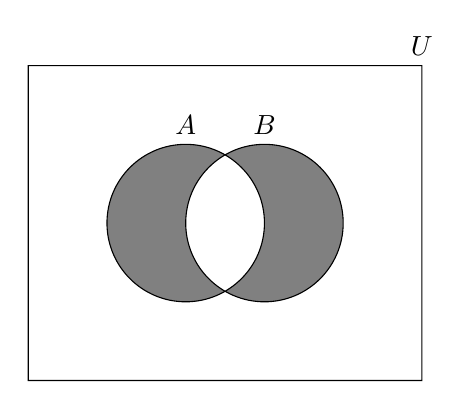
\begin{tikzpicture}[fill=gray]
                \scope
                \clip (-2,-2) rectangle (2,2)
                      (1,0) circle (1);
                \fill (0,0) circle (1);
                \endscope
                \scope
                \clip (-2,-2) rectangle (2,2)
                      (0,0) circle (1);
                \fill (1,0) circle (1);
                \endscope
                \draw (0,0) circle (1) (0,1)  node [text=black,above] {$A$}
                      (1,0) circle (1) (1,1)  node [text=black,above] {$B$}
                      (-2,-2) rectangle (3,2) node [text=black,above] {$U$};
            \end{tikzpicture}
        \end{center}
    \end{frameddefn}

    \begin{framedprop}[label={prop diff simm}]{Differenza simmetrica vuota}
        Dati due insiemi $A$ e $B$, si ha che $$A \ \Delta \ B = \varnothing \iff A = B$$
    \end{framedprop}

    \proofiff{
        Per assurdo, sia $A \ \Delta \ B = \varnothing$ e $A \neq B$; si noti che $A \neq B$ se e solo se esiste $x \in A - B$, oppure $x \in B - A$, e dunque

        \begin{itemize}
            \item $x \in A - B \implies x \in A \land x \notin B \implies x \in A \cap \lnot B \implies A \ \Delta \ B \neq \varnothing$ $\lightning$
            \item $x \in B - A \implies x \in B \land x \notin A \implies x \in \lnot A \cap B \implies A \ \Delta \ B \neq \varnothing$ $\lightning$
        \end{itemize}
    }{
        Per dimostrare la tesi, è sufficiente considerare che $$A = B \implies A \cap \lnot B = \lnot A \cap B = \varnothing \implies A \ \Delta \ B = \varnothing$$
    }

    \begin{framedthm}{Decidibilità di $EQ_\DFA$}
        $EQ_\DFA$ è decidibile; in simboli $$EQ_\DFA := \{\abk{A, B} \mid A, B \in \DFA : L(A) = L(B) \} \in \DEC$$
    \end{framedthm}

    \begin{proof}
        Sia $M$ una macchina di Turing; una volta controllata la validità della codifica in input, $M$ può convertire i due \DFA $A$ e $B$ forniti in input in un terzo \DFA $C$ --- utilizzando gli algoritmi presentati all'interno della \cref{closure unione}, della \cref{closure inters} e della \cref{closure compl} --- tale che $$L(C) = L(A) \ \Delta \ L(B)$$ e dunque per la \cref{prop diff simm}, si ha che $$L(A) = L(B) \iff L(C) = \varnothing = \emptyset$$ Sia $M'$ la \TM costruita all'interno del \cref{dec e_dfa}; allora, $M$ può utilizzare $M'$ sull'input $\abk{C}$, poiché se $M'$ accetta, allora $L(C) = \emptyset$, e dunque $A$ è equivalente a $B$; allora $M$ accetta se e solo se $M'$ accetta, e poiché $M'$ è decisore per la dimostrazione del \cref{dec e_dfa} stessa, segue la tesi.
    \end{proof}

    \begin{framedthm}{Indecidibilità di $EQ_\CFG$}
        $EQ_\CFG$ è indecidibile; in simboli $$EQ_\CFG := \{\abk{G,H} \mid G,H \in \CFG : L(G) = L(H)\} \notin \DEC$$
    \end{framedthm}

    \begin{proof}
        Omessa.
    \end{proof}
\end{document}
